%% 
%% Copyright 2019 Elsevier Ltd
%% 
%%
%%%%%%%%%%%%%%%%%%%%%%%%%%%% ! ! ! SUBMISSION CHECKLIST ! ! ! %%%%%%%%%%%%%%%%%%%%%%%%%%%%
%%
%% Please confirm that your submission follows all the requirements of the guidelines, including the submission checklist:
%% _ Cover letter
%% _ Highlights
%% _ Authorship statement
%% _ The manuscript must be single column and double spaced
%% _ Reference must be in the author-date format
%% _ Code availability section 
%%
%% *All the manuscripts in disagreement with the guidelines will be desk-rejected without editorial check.
%%
%% --------------------------------------
%%
%% This file is part of the 'CAS Bundle'.
%%  
%% It may be distributed under the conditions of the LaTeX Project Public
%% License, either version 1.2 of this license or (at your option) any
%% later version.  The latest version of this license is in 
%%    http://www.latex-project.org/lppl.txt 
%% and version 1.2 or later is part of all distributions of LaTeX
%% version 1999/12/01 or later.
%%   
%% The list of all files belonging to the 'CAS Bundle' is
%% given in the file `manifest.txt'.
%% 
%% Template article for cas-dc documentclass for  
%% double column output.
 
%\documentclass[a4paper,fleqn,longmktitle]{cas-dc}
\documentclass[a4paper,fleqn]{cas-sc}

\usepackage[authoryear]{natbib}
\usepackage{graphicx} 
\usepackage{float}
\usepackage{algorithm}  
\usepackage{algpseudocode}
\usepackage{color}
\usepackage{subfigure}
\usepackage{setspace}
\usepackage{float}
\usepackage{diagbox}

\usepackage[nomarkers,figuresonly]{endfloat}


\newcommand{\colorComments}{black} 
 
%%%Author definitions
\def\tsc#1{\csdef{#1}{\textsc{\lowercase{#1}}\xspace}}
\tsc{WGM}
\tsc{QE}
\tsc{EP}
\tsc{PMS}
\tsc{BEC}
\tsc{DE}
%%%

\usepackage{lineno}
\linenumbers 

\begin{document}
\let\WriteBookmarks\relax
\def\floatpagepagefraction{1}
\def\textpagefraction{.001}
\shorttitle{Combining class-weighted algorithm and machine learning models in landslide susceptibility mapping}
<<<<<<< HEAD
\shortauthors{Yingxu Song et al}
=======
\shortauthors{Huijuan Zhang et al}
>>>>>>> d17d830d74a41a28a19dec78c81ba8068dd4bd0f

\title [mode = title]{Comparison of deep learning methods and ensemble learning methods in the evaluation of landslide susceptibility}

\author[1]{Yingxu Song} [type=editor,
auid=000,bioid=1,orcid=0000-0002-9273-2019]
\credit{Conceptualization, Methodology, Software, Validation, Investigation, Resources, Funding acquisition}

\author[2]{Huijuan Zhang}[]
\credit{Conceptualization, Validation, Writing-original draft preparation, Writing-review and editing}

\author[4]{Shiluo Xu}
\credit{Software, Resources}

\author[5]{Yueshun He}
\credit{Project administration, Funding acquisition}

\author[6]{Zhiwen Li}
\credit{Conceptualization}

\author[7]{Xianyu Yu}
\credit{Resources, Funding acquisition}

\author[8]{Ye Liang}
\credit{Funding acquisition}

\author[1]{Weicheng Wu}
\credit{Writing-review and editing}

\author[2]{Yue Wang}
\credit{Software}

\address[1]{Jiangxi Engineering Laboratory on Radioactive Geoscience and Big Data Technology, School of Information and Engineering, East China University of Technology, Nanchang, 330013, Jiangxi, China; yxsong@ecut.edu.cn}
\address[2]{School of Earth Sciences, East China University of Technology, Nanchang, Jiangxi Province 330013, China}
\address[3]{Key Lab of Digital Land and Resources and Faculty of Earth Sciences, East China University of Technology, Nanchang, 330013, Jiangxi, China}
\address[4]{School of Information Engineering, Huzhou University, Huzhou 313000, China; xushiluo@163.com} 
\address[5]{East China University of Technology, Nanchang, 330013, Jiangxi, China; heys@ecut.edu.cn} 
\address[6]{School of Environmental and Chemical Engineering, Foshan University, Foshan, 528000, China; lizw1982@163.com} 
\address[7]{School of Civil Engineering, Architecture and Environment, Hubei University of Technology, Wuhan, Hubei Province 430074, China; yuxianyu@hbut.edu.cn} 
\address[8]{Jiangxi Engineering Technology Research Center of Nuclear Geoscience Data Science and System, East China University of Technology, Nanchang, 330013, Jiangxi, China; liangye@ecut.edu.cn} 
\address[1]{Key Lab of Digital Land and Resources and Faculty of Earth Sciences, East China University of Technology, Nanchang, 330013, Jiangxi, China; wuwch@ecut.edu.cn/wuwc030903@sina.com} 
\address[2]{School of Earth Sciences, East China University of Technology, Nanchang, Jiangxi Province 330013, China; 2020210058@ecut.edu.cn} 


\begin{abstract}
This study aims to investigate the application of the class-weighted algorithm combined with traditional machine learning (logistic regression) and ensemble machine learning models (LightGBM and random forest) to the landslide susceptibility evaluation. 
Wanzhou section of the Three Gorges Reservoir area, China, which have numerous landslides and the number of landslide samples is 19 times more than non-landslide samples, is chosen as an example. 
The class-weighted algorithm focuses on the class-imbalanced problem of landslide and non-landslide samples in the assessment of landslide susceptibility and can turn the class-imbalanced issue into a cost-sensitive problem by setting unequal weights for different classes, which contribute to improving landslide susceptibility evaluation accuracy.   
The landslide inventory database was produced by field investigation and remote sensing images derived from Google Earth. 
Of the 233 landslides in the inventory, 40\% were used for validation, and the remaining 60\% were used for training purposes. 
Twelve environmental parameters (elevation, slope, aspect, curvature, distance to river, NDVI, NDWI, rainfall, seismic intensity, land use, TRI, lithology) were treated as inputs of the models to produce landslide susceptibility map (LSM). The AUC value, Balanced accuracy, and Geometric mean score were utilized to estimate the quality of models. 
The results showed that the weighted models (weighted logistic regression, weighted LightGBM, weighted random forest) have higher AUC values, Balanced accuracy, and Geometric mean scores than those of unweighted methods, which demonstrated that the weighted models exhibit better than unweighted methods, with the weighted random forest method having the best performance. 
The landslide susceptibility map of the Wanzhou section display that the high and very high landslide susceptibility are mainly distributed on both sides of the river. 
The insights from this research will be useful for ameliorating the landslide susceptibility mapping and the development of prevention and mitigation Wanzhou section. 
\end{abstract}
 
\begin{coverletter}

Dear Editors-in-Chief,
\newline

please find the enclosed manuscript "Combining class-weighted algorithm and machine learning models in landslide susceptibility mapping: a case study of Wanzhou section of the Three Gorges Reservoir, China" which we are submitting for exclusive consideration for publication in Computers \& Geosciences. 
We confirm that the submission follows all the requirements and includes all the items of the submission checklist.  
\newline

In this contribution, to solve the imbalanced landslide samples (landslides, non-landslides) in the landslide susceptibility evaluation, the application of the class-weighted algorithm combined with traditional machine learning (logistic regression) and ensemble machine learning models (LightGBM and random forest) have been investigated. 
Wanzhou section of the Three Gorges Reservoir area, China, where the number of landslide samples is 19 times more than non-landslide samples, is chosen as an example. 
The landslide inventory database was produced using field investigation and remote sensing images provided by Google Earth. 
Of the 233 landslides in the inventory, 40\% were used for validation, and the remaining 60\% were used for training purposes. Twelve environmental parameters (elevation, slope, aspect, curvature, distance to river, NDVI, NDWI, rainfall, seismic intensity, land use, TRI, lithology) were used as inputs of the models to produce landslide susceptibility map (LSM). 
The AUC value, Balanced accuracy, and Geometric mean score were used to estimate the quality of models. 
Research has found that the weighted models (weighted logistic regression, weighted LightGBM, weighted random forest) are better than unweighted methods and the weighted random forest method has the best performance. 
The class-weighted algorithm turned the susceptibility evaluation problem into a cost-sensitive problem by setting unequal weights for different classes, which is probably to be applied to the landslide susceptibility evaluation in other areas.
\newline

We provide the source codes in a public repository with details listed in the section "Code availability".
\newline

Thanks for your consideration. 
\newline
Sincerely,
\newline

Yingxu Song
\newline
Jiangxi Engineering Laboratory on Radioactive Geoscience and Big Data Technology, School of Information and Engineering, East China University of Technology, Nanchang, 330013, Jiangxi, China; yxsong@ecut.edu.cn
\end{coverletter}

 
\begin{highlights}
\item The imbalanced landslide samples (landslides, non-landslides) in the landslide susceptibility evaluation is emphasized.
\item The class-weighted algorithm combined with machine learning (Logistic regression) and ensemble machine learning models (LightGBM and random forest) were applied to the landslide susceptibility evaluation.
\item The weighted models are applicable for solving the problem of imbalanced landslide samples and have improved the landslide susceptibility mapping well.
\end{highlights}

\begin{keywords}
landslide susceptibility mapping\sep class-weighted algorithm \sep imbalanced landslide data \sep machine learning model \sep Three Gorges Reservoir area
\end{keywords}

\maketitle 

\printcredits

\doublespacing


\section{Introduction}

Landslide refers to a natural phenomenon in which the soil or rock mass on the slope slides downwards along the soft surface under the action of gravity or other external forces.
Landslide is a common geological disaster, causing many economic losses and unfor-tunate casualties, such as devastating soil, vegetation, and dwellings, as well as critically blocking transportation lines and waterways \citep{Abuzied2016JoMS, 2017Chenp147160}.
The China Geological Survey reported that there were 6181 geological disasters in 2019, including landslides, collapses, mudrock flows, the ground collapses, ground fissures, and land subsidence, resulting in 211 deaths, 13 missings, 75 injured and direct economic losses of 2.77 billion Yuan.
Among them, 4020 landslides occurred, mainly distributed in Southwestern China, and brought about a large number of missing persons and severe economic losses.
Various factors, such as natural factors (e.g., heavy rainfall, earthquake, loose lithology, and low vegetation coverage, etc.) and human-made factors (e.g., infrastructures construction and road irrigation, etc.) can trigger landslides \citep{2018Wildep97104}.
Especially in recent years, the rapid urbanization and industrialization have increased the likelihood of landslide occurrence \citep{2020Kocamanp118}, which led to higher number of human casualties and more enormous loss of property. 
It is therefore of significant necessity to develop landslide susceptibility map, which represents the probability of the spatial distribution of landslides in a specific region based on historical landslides and related factors \citep{Yu2016IJERPH,Song2018}.
Government agencies have attempted to take various measures to reduce the casualties and financial losses caused by landslides. 
This process generally involves carrying out LSM, representing the probability of the spatial distribution of landslides in a specific region based on historical landslides and related factors \citep{Yu2016IJERPH,Song2018}. 
Landslide susceptibility map can help government agencies to take preventable measures for reducing the casualties and financial losses caused by landslides.

Various methods and techniques, which can be defined as qualitative or quantitative, have been implemented in the landslide susceptibility assessment and have achieved notable progress \citep{Fang2020IJoGIS,Guzzetti_1999_Geomorphology,Bui2020Catena}. 
Qualitative methods are based on expert knowledge to identify the main triggering factors, determine the weights of natural and human-made factors and acquire landslide susceptible zones \citep{Aditian2018Geomorphology}, such as analytic hierarchy process (AHP) (Barredo et al., 2000; Yalcin, 2008; Feizizadeh et al., 2014)\citep{Barredo2000IJoAEOaG,Yalcin2008Catena}, interval pairwise comparison matrix (IPCM)\citep{Ghorbanzadeh2019RemoteSensing}, and fuzzy logic models\citep{Aksoy2012Computers&Geosciences,Anbalagan2015GeoenvironmentalDisasters,Shahabi2015EnvironmentalEarthSciences,Roy2019RemoteSensingApplicationsSocietyandEnvironment}. 
Whereas quantitative methods rely on mathematical models including the statistical and deterministic models\citep{Abuzied2016JoMS, Reichenbach2018ER,Fang2020IJoGIS}. 
With the rapid advancement of computer technology and the improvement of remote sensing (RS) and geographic information system (GIS) technology, the quantitative methods develop swiftly. 
Many studies have demonstrated that the quantitative approaches are more precise than qualitative methods because the qualitative methods have much subjectivity concerning the prediction of landslides\citep{Aditian2018Geomorphology, Bui2020Catena}. 
Machine learning model which is one of the qualitative methods has the capability of handling non-linear data with different scales and from different type of sources\citep{Bui2020Catena}. 
Different machine learning algorithms together with GIS and RS techniques have been widely applied to assess landslide susceptibility and perform well, such as LR (logistic regression), which were most widely used and often found successful in the landslide susceptibility evaluation \citep{Ayalew2005Geomorphology,Eeckhaut2006Geomorphology,Bai2010Geomorphology,Akgun2012Landslides,Sevgen2019S,Dag2020EES}. 
Additionally, the ensemble learning methods acting as an improvement of traditional machine learning models arise and show more robust performance in many real-world tasks, widely used in landslide susceptibility evaluation \citep{Althuwaynee2014Landslides,Napoli2020Landslides,Hong2020SoTTE,Saha2021SoTTE}. 
<<<<<<< HEAD
Random forest (RF) \citep{Breiman2001}, which is an extended variant of the bagging method, has a simple implementation and low computational overhead \cite{Youssef2015Landslides, Kim2017GI}. 
=======
Random forest (RF) \citep{Breiman2001}, which is an extended variant of the bagging method, has a simple implementation and low computational overhead \citep{Youssef2015Landslides, Kim2017GI}. 
>>>>>>> d17d830d74a41a28a19dec78c81ba8068dd4bd0f
LigthGBM is a new member of the boosting ensemble models, having faster training efficiency, higher accuracy, and more robust ability to handle large-scale data \citep{Song2018}. 

The choice of samples seriously affects the accuracy of the machine learning models. 
Some researchers have paid attention to the sample selection in the evaluation of landslide susceptibility, polygon-based random sampling (PBRS) \citep{San2014IJoAEOaG}, two-level random sampling (2LRS) \citep{Ada2017NH, Aktas2019C&G} were used to produce more realistic landslide susceptibility maps.

However, the area of the landslide area is often much smaller than that of the non-landslide area. 
Selecting the same amount of samples under different categories will often result in underrepresentation of non-landslide samples, waste of non-landslide samples and loss of important information, lead to poor performance in landslide susceptibility evaluation models.

The class-weighted algorithm treats the susceptibility assessment as a cost-sensitive issue and sets different misclassification weights for different categories (landslides, non-landslides). 
This method has been widely used to solve the unbalanced variety, but the application to landslide susceptibility assessment is still relatively few.



Wanzhou district of Chongqing is in the Three Gorges Reservoir area's hinterland, playing a significant role in the prevention and domination of geological disasters in the Three Gorges Reservoir area. 
In recent decades, because of the abundant precipitation and cyclical fluctuation of water level in the Yangtze River, landslides and other geological disasters in this area have increased significantly, seriously destroying the ecological environment and socially sustainable development. 
In this study, the Wanzhou section of Three Gorges Reservoir was selected as the research area, and the class-weighted algorithm combined with traditional machine learning model (Logistic regression) and ensemble machine learning models (LightGBM and random forest) were applied to the landslide susceptibility evaluation. 
<<<<<<< HEAD
The purpose of this research attempts to achieve the relatively optimal method in which the impact of unbalanced landslide samples can be minimized, and the accuracy of the landslide susceptibility map is improved, providing essential introductory information for mitigating the land-slide hazard by governmental subdivisions or decision-makers. 
=======
The purpose of this research attempts to achieve the relatively optimal method in which the impact of unbalanced landslide samples can be minimized, and the accuracy of the landslide susceptibility map is improved, providing essential introductory information for mitigating the landslide hazard by governmental subdivisions or decision-makers. 
>>>>>>> d17d830d74a41a28a19dec78c81ba8068dd4bd0f
Different from previous work, the novelty of this paper are 1) the class-weighted algorithm is firstly applied to landslide susceptibility mapping; 2) the advantages and disadvantages of traditional machine learning model (Logistic regression) and ensemble machine learning models (LightGBM and random forest) combined with class-weighted algorithm were compared in the Wanzhou section.

\section{Study area and data used}

Wanzhou District belonging to Chongqing Municipality, is in the hinterland of the Three Gorges Reservoir area. 
The terrain of Wanzhou District is mostly mountains and hills, with large topographic fluctuations which is largely attributed to its location at the eastern margin of East Sichuan Fold belt. 
Additionally, the study area is located in the Yangtze River Valley, and the floodplain landform is widely developed, forming a typical river terrace landform. The existence of river terraces and low mountain hills makes the area widely developed with various slopes, which is more conducive to the occurrence of landslide disasters.
<<<<<<< HEAD
The study area with 223 historical landslides (Figure 1a) is the bank section of Wanzhou District, having many rivers and streams of the Yangtze River system \citep{Yu2016IJERPH,Song2018}. 
=======
The study area with 223 historical landslides (\ref{StudyArea}a) is the bank section of Wanzhou District, having many rivers and streams of the Yangtze River system \citep{Yu2016IJERPH,Song2018}. 

\begin{figure}
  \centering
  \includegraphics[width=12 cm]{Definitions/Fig1_study_area.eps}
  \caption{Location of the study area. (\textbf{a}) Elevation of the study area. (\textbf{b}) Three Gorges Reservoir area. (\textbf{c}) Wanzhou District, the image is a Landsat 8 image with true color (R:band 4; G: band 3; B:band 2).}
  \label{StudyArea}
\end{figure}  
  
% Figure_lithology
\begin{figure}
  \centering
  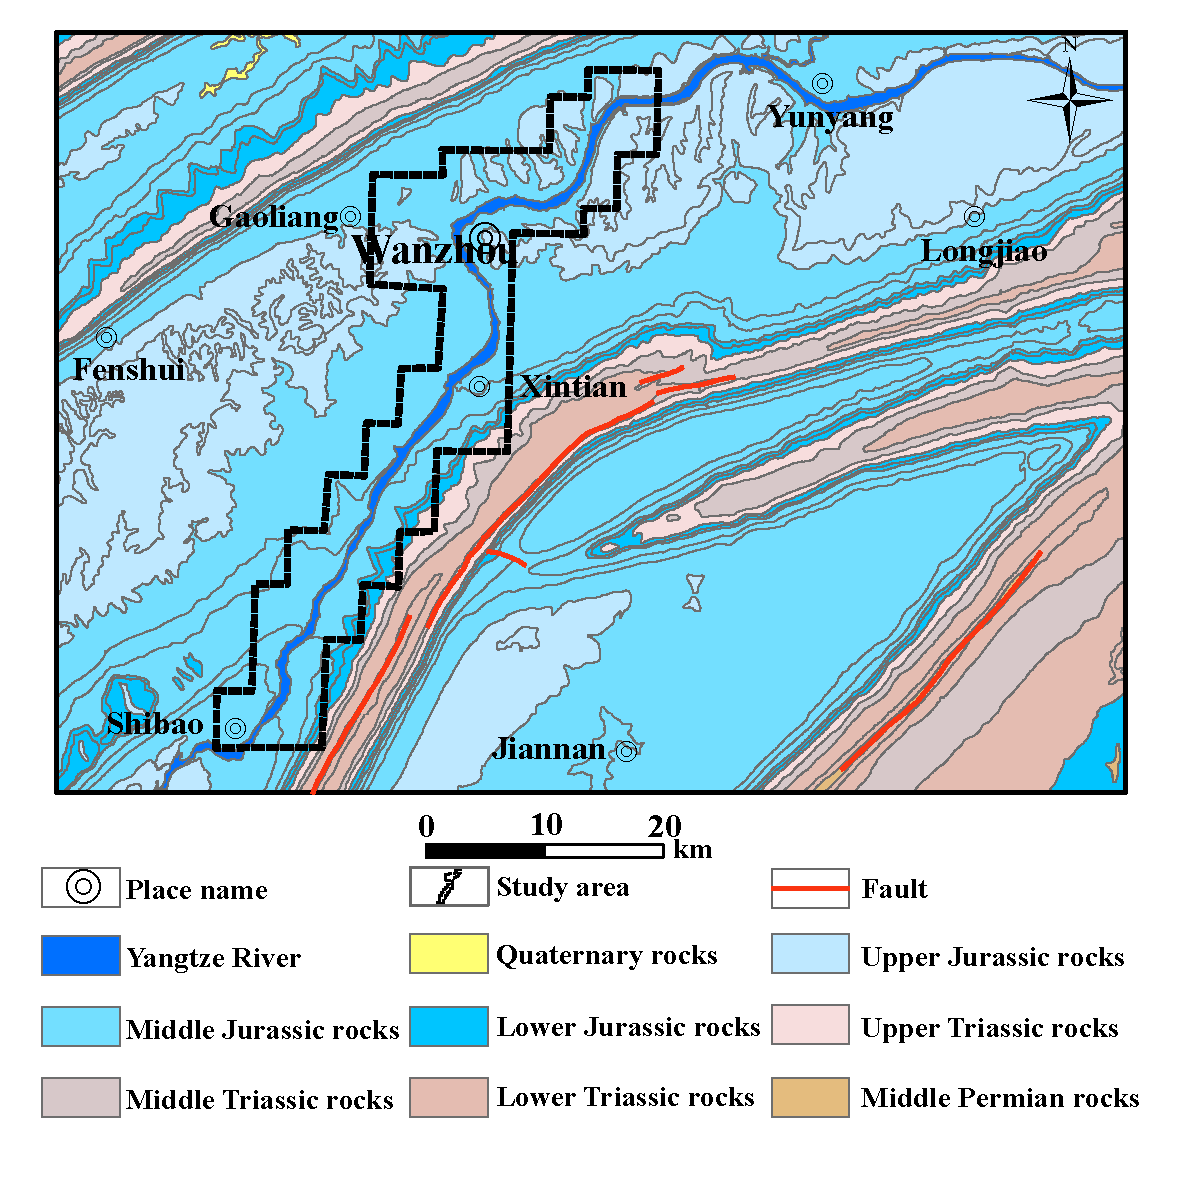
\includegraphics[width=12 cm]{Definitions/Fig2_Stratigraphic_map.eps}
  \caption{The geological and tectonic sketch of the study area.}
  \label{Fig_Lithology}
\end{figure} 

>>>>>>> d17d830d74a41a28a19dec78c81ba8068dd4bd0f
Wanzhou District is in the subtropical monsoon region with plentiful precipitation. 
The rainfall is mainly concentrated from May to September, which accounts for about 60\% of the annual rainfall, triggering abundant landslides. 
The rivers and streams in Wanzhou District have deep cuts, large drops, and branch-like distribution, all of which belong to the Yangtze River system. 
The rivers in the territory with a drainage area of more than 100 $km^{2}$ include the Zhuxi River, Duhe River, Shiqiao River, Ruxi River, and Puli River in northern of the Yangtze River, and Nixi River, Wuqiao River and Xintian River in southern of the Yangtze River. 
Wanzhou District is located in the northwest edge of the Sichuan-Hubei-Hunan uplift fold belt of the first-class structure of the Neocathaysian system, mainly including Changliangzi anticline and its syncline, Yushan anticline, Qiyaoshan anticline and Hengshixi anticline in the East. 
A number of tectonic fissures are distributed in NNE or NE direction. There are Triassic, Jurassic and Quaternary strata (including alluvial deposits and slope deposits, etc.) in the study area \citep{Song2018}. 
<<<<<<< HEAD
=======

>>>>>>> d17d830d74a41a28a19dec78c81ba8068dd4bd0f
The lithology is relatively complicated, and the particles can be divided into shale and sand-mudstone interbedded, mudstone, siltstone, sandstone, red clastic rock according to the material composition. 
The lithology is characterized by soft and hard phases, low mechanical strength, and obvious differential weathering, which provides favorable materials for the landslides. 
Wanzhou District is subordinate to the weak seismic zone in southern China, and thus lacks any notable threat of earthquakes to local geo-hazards. 
The combination of the above natural environmental characteristics and human influences (such as accelerating engineering construction and increasing population) leads to some geo-hazards in Wanzhou District, especially landslides. 
The landslide data mainly come from landslide geological surveys and the remote sensing images provided by Google Earth. 
The DEM data with 30 $\times$ 30 m resolution derived from Aster GDEM. 
A Landsat-8 satellite image which was acquired on 2013-08-12 were utilized as primary remote sensing data. 
<<<<<<< HEAD
Table 1 shows the types and sources of data in this study. 
A total of 12 landslide contributing factors and the types of data were shown in Table 2. 
Figure 3 shows the distributions of twelve landslide factors. 
Elevation, slope, aspect, curvature, and topographic roughness index (TRI) were derived from the DEM data using the ArcGIS and QGIS. The lithological data and the distance to the river were vectorized from the geological and topographic maps. 
The NDVI/NDWI data were acquired from the Landslide 8 OLI images. 
The rainfall data were provided by the Meteorological Bureau. 
The land-use data came from the geological survey and the Landslide 8 OLI images.

\section{Methodology}

The flowchart of landslide susceptibility mappingfor the study area is shown as in Fig. 4. 
Firstly, twelve landslide contributing factors and landslide samples were selected as independent variables and dependent variables, respectively, to form an initial decision table for training the models. 
Not all the landslide contributing factors are indispensable for the landslide susceptibility assessment (Dou et al., 2015). 
Therefore, multicollinearity analysis of landslide contributing factors is essential for improving the robustness of the models. 
In this study, the variance inflation factor method (VIF) was utilized to carry out multicollinearity analysis of landslide conditioning factors. 
Secondly, a so-called "Pipeline" strategy was used to connect data processing and classifiers. 
The disposing of data includes factor-normalization and factor-reduction in which the StandardScaler function and PCA method provided by Sklearn were implemented (Pedregosa et al., 2011). 
The purpose of employing "Pipeline" is to ensure the consistency of the data preprocessing in the training set and test set. 
Thirdly, the traditional machine learning (logistic regression) and ensemble machine learning models (LightGBM and random forest) were applied to achieve the landslide susceptibility mapping. 
Finally, several evaluation indicators (e.g., AUC value, balanced accuracy, and geometric mean score) were implemented to evaluate the LSM models.


\subsection{Logistic Regression (LR)}

Logistic regression (LR) is a classic machine learning model with the capacity to settle classification problems \citep{Ayalew2005Geomorphology,Bai2010Geomorphology,Song2018}. 
It is widely used in landslide susceptibility evaluation because of its simplicity, parallelization, and strong interpretability. 
Logistic regression can be treated as a variant of linear regression, and the variables of the LR model could be continuous or discrete \citep{Ayalew2005Geomorphology,Bai2010Geomorphology}. 
The core concept of logistic regression is to map the domain's value from (-$\infty$, +$\infty$) to (0,1). 
0 and 1 represent different categories, respectively. 
They represent non-landslides (0) and landslides (1) in the landslide susceptibility evaluation. 
A Sigmoid function is employed to express this mapping relationship, as shown below (Equation \ref{eqn:gz}).

\begin{equation}
  g(z)=\frac{1}{1+e^{-z}}
  \label{eqn:gz}
\end{equation}

\subsection{LightGBM}

LightGBM is a new gradient boosting framework proposed by Microsoft \citep{Friedman2002_GBoost}. 
LightGBM belongs to the Boosting family in ensemble learning and relies on decision tree algorithms. 
LightGBM is widely used for classification tasks and machine learning competitions because of its higher efficiency and lower memory usage than other gradient boosting frameworks (e.g., Adaboost, GBDT, etc.). 
The application of LightGBM addresses the problems encountered by GBDT in massive data and en-sures the better performance of GBDT in industrial practice.

\subsection{Random Forests (RF)}

The RF method belongs to the Bootstrap aggregation, a basic ensemble learning model \citep{Breiman2001}. 
Random forests have a simple implementation, low computational overhead, and robust performance in many machine learning tasks. 
The diversity of Bagging basic learners comes from sample perturbations and attributes perturbations, further improving the generalization performance of the final integration \citep{Youssef2015Landslides}. 

\subsection{Class-weighted machine learning models}

When the samples of landslide and non-landslide are equal or similar, the machine learning will have excellent performance. 
Otherwise, the process of machine learning will be seriously affected by imbalanced samples. 
The imbalance of categories may cause the predictive results to be biased towards the side with more sample categories: the non-landslide area. 
If the landslide area is predicted as a non-landslide area, the accuracy and practicability of the landslide sensitivity evaluation result will be low. 
For example, there are 98 negative examples (non-landslides) but only 2 positive examples (landslides). 
The learning model only requires returning a learner that always predicts new samples as negative examples, which can achieve 98\% accuracy. 
However, such learners are worthless because they cannot predict any positive cases.
The class-imbalanced problem can be solved by oversampling positive samples (landslides), undersampling negative samples (assuming the non-landslide is the majority class) or treating the machine learning process as a cost-sensitive learning problem. 
The representative oversampling methods are the SMOTE and Borderline-SMOTE, while the representative undersampling technique is the EasyEnsemble method (Verbiest et al., 2014). 
The oversampling method's time overhead is usually more than that of the undersampling method because the former method adds many positive examples and makes the classifier training set much larger than the initial training set. 
Moreover, the oversampling method cannot simply repeat the initial the sampling of the initial positive samples, leading to serious overfitting. 
Although the undersampling method can reduce time overhead by randomly discarding the negative examples, some critical information might be lost during this process. 
When viewed as a cost-sensitive issue, the class-imbalanced problem could be well solved because a so-called cost matrix used in the machine learning process can set the weights corresponding to different categories for improving the accuracy of classification. 
The class-weighted machine learning methods used in this article belong to this category.
In this study, the entire study area was resampled into 553,172 non-landslide samples and 29,313 landslide samples. 
The ratio of non-landslide samples to landslide samples was approximately 19:1. 
Therefore, the LSM process in this study should be regarded as a typical class-imbalanced problem. 
Table 3 shows the cost matrix used in this study.

\subsection{Model elevation}
\subsubsection{Confusion matrix and ROC curve}

The confusion matrix is comprised of the following four indexes: true positive (TP), false positive (FP), true negative (TN), and false negative (FN). 
Various statistical indicators, including accuracy (Equation \ref{eqn:ACC}), TPR/recall (Equation \ref{eqn:TPR}), TNR (Equation \ref{eqn:TNR}), ROC curve (Receiver Operating Characteristic), and AUC (area under ROC curve), could be calculated through the above four indexes. 
These indicators are usually employed to evaluate the performance of machine learning tasks, consisting of land-use classification \citep{Jr2014IJoGIS}, LSM, etc.

\begin{equation}
  \text { Accuracy }=\frac{T P+T N}{T P+F P+T N+F N}
  \label{eqn:ACC}
\end{equation}

\begin{equation}
  T P R=\text { Sensitivity }=\text { Recall }=\frac{T P}{T P+F N}
  \label{eqn:TPR}
\end{equation}

\begin{equation}
  T N R=\text { Specificity }=\frac{T N}{T N+F P}
  \label{eqn:TNR}
\end{equation}

\subsubsection{Balanced accuracy and G-mean score}

In the cost sensitivity problem, the ROC curve cannot directly reflect the models' pros and cons. 
Thus, we used balanced accuracy and G-mean score provided by Sklearn (Pedregosa et al., 2011) as the evaluation indexes. The balanced accuracy (Equation \ref{eqn:BA}) in classification problems is defined as the average recall (TPR) obtained under each class, and the G-mean (Equation \ref{eqn:G_mean}) is the root of the product of TPR and TNR. 

\begin{equation}
  \text { Balanced Accuracy }=\frac{T P R+T N R}{2}
  \label{eqn:BA}
\end{equation}

\begin{equation}
  G-\text { mean }=\sqrt{T P R * T N R}
  \label{eqn:G_mean}
\end{equation}

\section{Results and discussions}
\subsection{Multicollinearity Analysis of Landslide Factors}

It is of great significance to employ multicollinearity analysis before landslide susceptibility modeling. 
Identifying and selecting appropriate landslide factors is the prerequisite for ensuring the robustness of these models. 
In this study, the variance inflation factor (VIF) was utilized to develop the multicollinearity analysis with the Python programming language (Table 4). 
If the value of VIF exceeds 10, meaning that there are multiple collinearities among variables. 
Results display that all the VIF values of the twelve factors are less than 10, denoting that all the 12 landslide-related factors are appropriate for LSM.

\subsection{Landslide susceptibility mapping results}

LR, LightGBM, RF models, and their weighted models (WLR, WLightGB, WRF) are utilized for landslide susceptibility mapping. 
Twelve landslide contributing factors: elevation, slope, aspect, curvature, distance to the river, NDVI, NDWI, rainfall, seismic intensity, land use, and topographic roughness index (TRI), and lithology were used as the input of these six models. 
The probability values of the six models range from 0 to 1, which are the so-called landslide prediction index values (LPI). 
The LPI values gener-ated by six models were reclassified to develop the landslide susceptibility map with the Natural Breaks method and the ArcGIS software. 
The landslide susceptibility maps (LR \& WLR, LightGBM \& WLightGBM, RF \& WRF) derived from the six models are shown in Figure 5 a–f. 
These landslide susceptibility maps (LSMs) are classified into very low, low, medium, high, and very high susceptibility to landslides. 

The percentages of each category in the six models are illustrated in Figure 6. 
In the LR case, the five landslide susceptibility classes of very low, low, medium, high, and very high covered 41.74\%, 31.55\%, 15.44\%, 8.57\%, and 2.70\% area of the districts, respectively. 
In the LightGBM and RF case, the class of very low area is much higher than those in LR case, while the class of low area is lower than those in LR case, and the classes of medium, high, and very high regions are almost the same as those in LR case. 
The percentages of very low and low classes in LR, LightGBM, and RF cases are higher than those in weighted models, but the percentage of very high and high areas in LR, LightGBM, and RF cases are lower than those in weighted models.

\subsection{Implications for landslide-prone Areas}

The regions with the high and very high landslide susceptibility are mainly distributed on both sides of the river (Figure 5), most likely related to the water level. Wanzhou reservoir area is the hinterland of the Three Gorges Reservoir area with the frequently variable water level. The rising water level of the Yangtze River can lead to the decrease of shear strength of the sliding body through softening and silting the slope (Wang and Qiao, 2013; Gui et al., 2016). In contrast, the drop in the water level produces a much larger hydrodynamic pressure, which increases the sliding force along the direction of underground seepage and then brings about the landslides (Wang and Qiao, 2013; Gui et al., 2016). There is the highest landslide susceptibility at the middle and lower reaches of the river (Figure 5). In addition to lithology, rainfall, and vegetation, the type of land-use is also probably to account for this characteristic. The strata exposed in the Wanzhou reservoir area are mainly Jurassic Shaximiao Formation (J2s) and Suining Formation (J3s) (Zhu et al., 2013). The lithology is off-white feldspathic quartz sand-stone intercalated with purplish-red argillaceous siltstone, purplish-red sandstone, and mudstone. It is easy to form a soft top and hard bottom structural surface because of the difference in weathering speed of mudstone and sandstone, providing an effective structure for the loose accumulation material sliding along the bedrock surface. Wan-zhou District is the center of a rainstorm in eastern Chongqing. According to the Datankou hydrological station's statistics, the average annual precipitation is 1243mm, and the maximum annual rainfall is about 1550mm (Yu et al., 2016; Song et al., 2018). The rainstorm strongly scours the landslide soil, infiltrate into cracks and potential sliding surfaces, resulting in the aggravation of landslide deformation. On the other hand, the rainfall will increase the slope's self-weight, thereby increasing the sliding force of the hill. Therefore, the combination of pore water pressure and soil softening can increase the probability of landslides (Finlay et al., 1997; Dahal et al., 2008). The plant roots have a powerful tensile effect on improving the anti-sliding ability of rock and soil, which anchor the loose weathered layer to the more stable rock and soil layer to prevent them from sliding along the slope. The plant stems and leaves, and litters can intercept and absorbing rainwater, which plays an inhibitory role in slope runoff and rain erosion (Sittadewi and Tejakusuma, 2019). However, the vegetation coverage of the research area is low, having a weak ability to resist landslides. The primary type of land-use in this area is wetland filled with groundwater, which is one of the significant external factors inducing landslide. Groundwater will sharply increase the weight of the rock and soil and reduce the anti-sliding resistance, which leads to the increase of sliding force and slope instability, resulting in landslides. Hence, LSM can be applied to land-use planning and in the prioritizing the management of countermeasures to mitigate potential losses by landslides and also helps the government formulate relevant scien-tific policies according to different susceptibility levels as a means of mitigating land-slides. Moreover, a LSM could also be used to raise public awareness of landslides and then reduce related activities in hazardous areas.

\section{Validation of landslide susceptibility maps}

The ROC curves of the six models are shown in Figure 7. The AUC values of the six models are 83.5%, 83.9%, 89%, 88.8%, 84.4%and 91.3%, respectively, indicating that all the six models are suitable for LSM in this region. Based on the ROC curves results, the weighted methods are generally better than the unweighted methods (except the LightGBM/WLightGBM), and the WRF model with the highest AUC value (AUC = 91.3%) is probably considered to be the most appropriate model.
The ROC curve cannot evaluate the models' performance perfectly because it cannot directly reflect the overall cost expectation of the models in case of unequal costs. Furthermore, the model's ability to predict landslides should be emphasized rather than non-landslides in the landslide susceptibility evaluation. Therefore, we selected more appropriate evaluation indicators to compare the pros and cons of the models. Table 5 shows the Balanced accuracy, G-mean, Recall, Accuracy, and AUC of the six models. The Recall values of the six models are 0.000, 0.774, 0.321, 0.842, 0.150 and 0.821, respectively. The Recall value of the LR model is 0, meaning that it cannot predict landslides. The weighted models (WLR, WLightGBM, WRF) are better than the un-weighted models (LR, LightGBM, RF) in terms of Recall, suggesting that the weighted models have a more powerful ability to predict landslides. The six models have dis-tinctive Accuracy values, with the figures of 0.950, 0.736, 0.952, 0.793, 0.950 and 0.772, respectively. The weighted models (WLR, WLightGBM, WRF) are worse than the unweighted models (LR, LightGBM, RF) in terms of Accuracy values, denoting that the unweighted models have the stronger ability to predict non-landslides. The G-mean values and Balanced accuracy values of the six models are 0.000, 0.774, 0.321, 0.842, 0.150, 0.821 and 0.500, 0.776, 0.550, 0.844, 0.511, 0.823, respectively. The G-mean and Balanced accuracy values imply that the weighted models are better than the unweighted models in LSM when a class-imbalanced problem is viewed as a cost-sensitive issue. In line with the AUC results, the Balanced accuracy and G-mean scores indicate that the WRF model has achieved much better performance than the other weighted models.
Landslide events not only reduce the financial losses but also cost human lives. A landslide susceptibility map is an essential tool for developing preventive measures in landslide-prone areas. Therefore, many scholars are committed to improving LSM models' performance. Recently, machine learning models and ensemble machine learning models had good performance in LSM. However, few studies have focused on the class-imbalanced problem, which will lead to poor performance in LSM whether the machine learning or ensemble machine learning models are utilized. Thus, we carried out the application of the class-weighted algorithm combined with traditional machine learning (LR) and ensemble machine learning models (LightGBM and RF) to the LSM based on a case study of the Wanzhou section of the Three Gorges Reservoir, China, in the present study. 
The results proved that the weighted methods (WLR, WLightGBM, WRF) are better than unweighted methods (LR, LightGBM, RF), shown as higher AUC, G-mean, and Balanced Accuracy values generally. Moreover, the WRF model has much better performance than WLR and WLightGBM models. Although the unweighted models have higher Accuracy value, they are incapable of evaluating landslide susceptibility because their accuracy rates come from the prediction of the negative class (non-landslides) rather than the positive class (landslides). A vital advantage of the weighted models is that the class-weighted algorithm turned the susceptibility evalua-tion problem into a cost-sensitive issue by setting unequal weights for different classes, which improves the performance of LSM, manifesting in higher Recall values. On the other hand, the weighted models (WLR/WLightGBM/WRF) tend to divide more high and very high susceptibility areas than the unweighted models (LR/LightGBM/RF) (Fig 5, 6). Landslide susceptibility map is the basis of landslide risk evaluation. Suppose the high susceptibility area is incorrectly classified as a low susceptibility zone, which may lead to a false judgment on the risk of landslides and then result in considerable threats to the safety of human life and property. Furthermore, the weighted models pay more attention to landslide samples' classification accuracy, which is the actual concern in the landslide susceptibility evaluation. Although every study area has its own unique landslide contributing factors and geological conditions, the weighted models proposed in this paper will provide significant clues for the landslide susceptibility evaluation concerning the imbalanced landslide samples. Regardless, the weighted models still have several disadvantages. For instance, the cost matrix should be processed before classification using weighted models, which is affected by the processing method and is time-consuming. Moreover, a high-resolution DEM for the study area is not freely available, resulting in the poor performance of weighted models. If high-resolution DEM were utilized for extracting landslide-related parameters, these weighted models could achieve better results. 
=======
Table \ref{tab_datasource} shows the formats and sources of data in this study. 

\begin{table}
  % \centering
  \caption{Data used, formats and sources}
  \begin{tabular}{lll}
    \toprule
    {\textbf{Data used}} & \textbf{Format} & \textbf{Source}\\
    \midrule
    \textbf{Historic Landslide} & Shapefile & geological survey and Google Earth software\\
    \textbf{DEM} & Tiff & Aster GDEM (\url{https://earthdata.nasa.gov/})\\
    \textbf{Landsat 8 OLI} & Tiff & USGS (\url{https://earthexplorer.usgs.gov/})\\
    \textbf{Lithology} & Shapefile & local Land and Resources Bureau\\
    \textbf{Meteorological data} & Shapefile & Meteorological Bureau (\url{http://www.cma.gov.cn/})\\
    \bottomrule
  \end{tabular}
  \label{tab_datasource}
\end{table}

A total of 12 landslide contributing factors and the types of data were shown in Table \ref{tab_factors}. 

\begin{table}
  \centering
  \caption{The names, types, and class of landslide impact factors.} 
  \begin{tabular}{llllll}
    \toprule
    \textbf{Variables} & \textbf{Name}  & \textbf{Variable type} & \textbf{Class} \\
    \midrule
    Y     & Landslide  & Binary & Landslide \\
    X1    & Elevation  & Continuous & Topography \\
    X2    & Slope  & Continuous & Topography \\
    X3    & Aspect  & Discrete & Topography \\
    X4   & Curvature  & Continuous & Topography \\
    X5   & Distance to river  & Continuous  & Hydrology \\
    X6   & NDVI   & Continuous & Land cover  \\
    X7   & NDWI   & Continuous & Land cover \\
    X8   & Rainfall  & Discrete & Triggered  \\
    X9   & Seismic intensity  & Discrete & Triggered  \\
    X10   & Land use  & Discrete & Triggered  \\
    X11   & TRI  & Continuous & Topography  \\
    X12   & Lithology  & Continuous & Topography  \\
    \bottomrule
    \end{tabular}%
  \label{tab_factors}%
\end{table}%

Figure \ref{Fig_Landslide_Factors} shows the distributions of twelve landslide factors. 
Elevation, slope, aspect, curvature, and topographic roughness index (TRI) were derived from the DEM data using the ArcGIS and QGIS. 
The lithological data and the distance to the river were vectorized from the geological and topographic maps. 
The NDVI/NDWI data were acquired from the Landslide 8 OLI images. 
The rainfall data were provided by the Meteorological Bureau. 
The land-use data came from the geological survey and the Landslide 8 OLI images.

\begin{figure}
  \centering
    \subfigure[~Elevation]{
    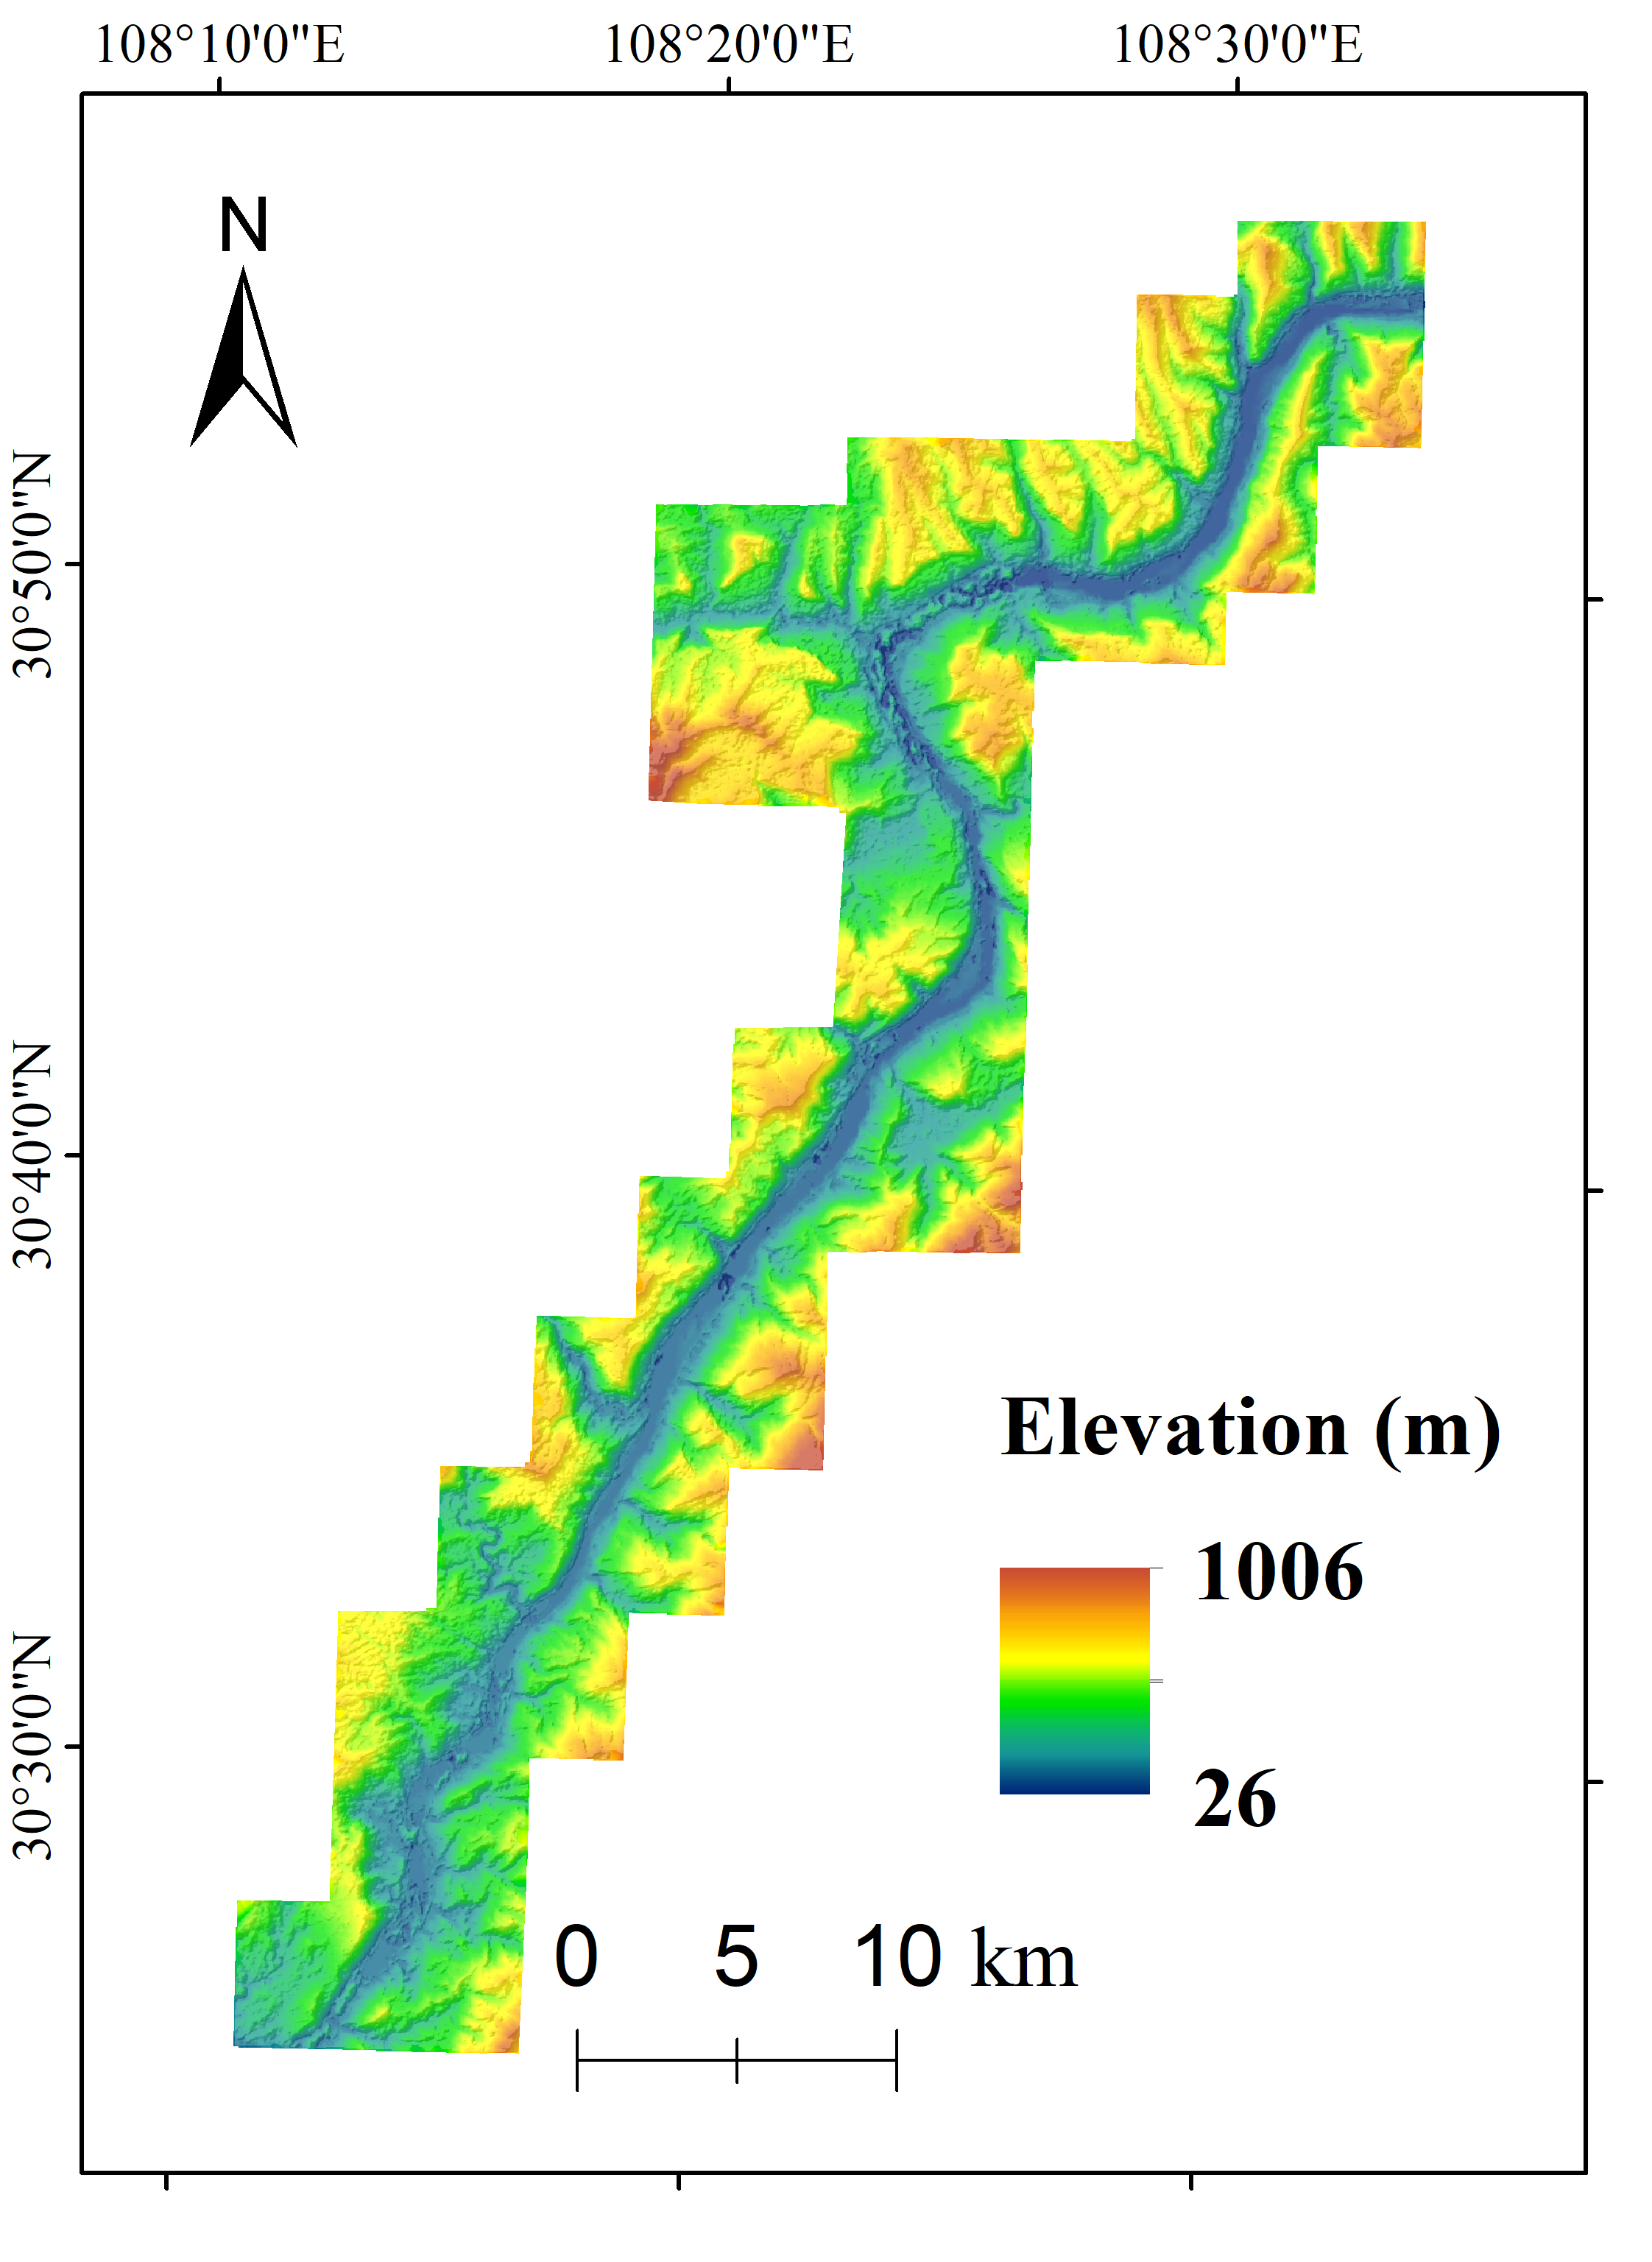
\includegraphics[width=4.5cm]{Definitions/Elevation.png}
    }
    \quad
    \subfigure[~Slope]{
    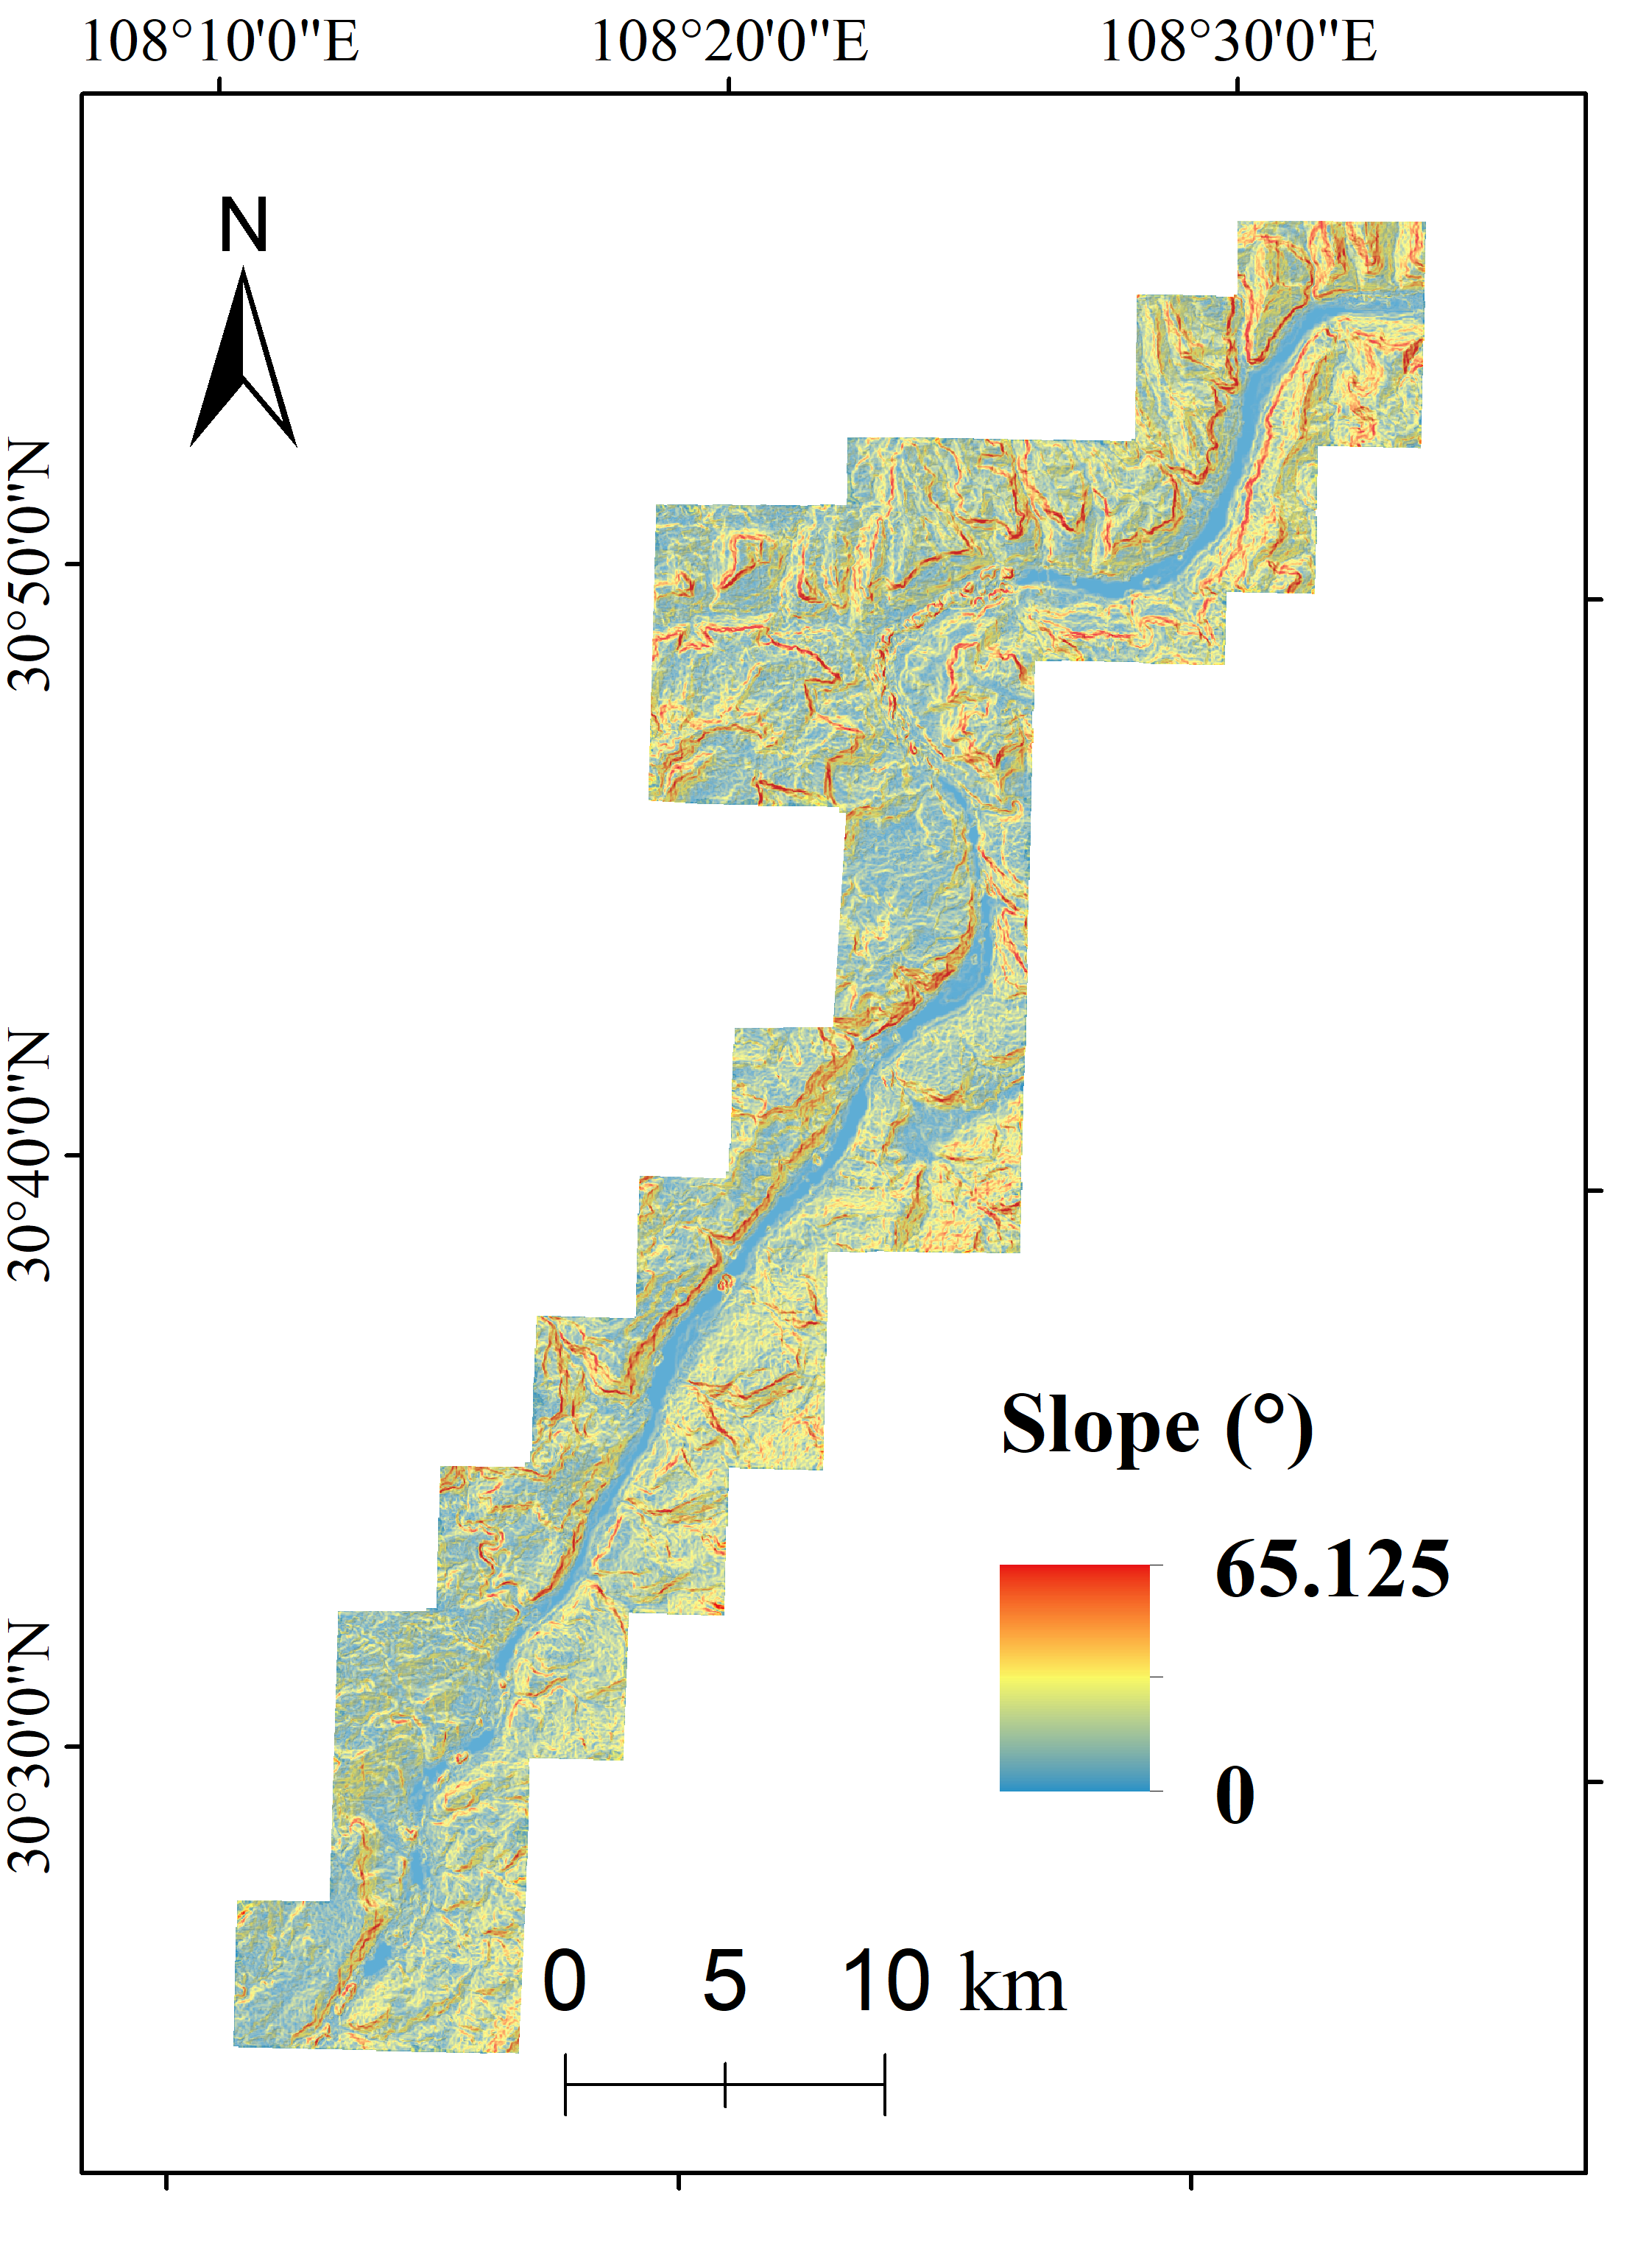
\includegraphics[width=4.5cm]{Definitions/Slope.png}
    }
    \quad
    \subfigure[~Aspect]{
    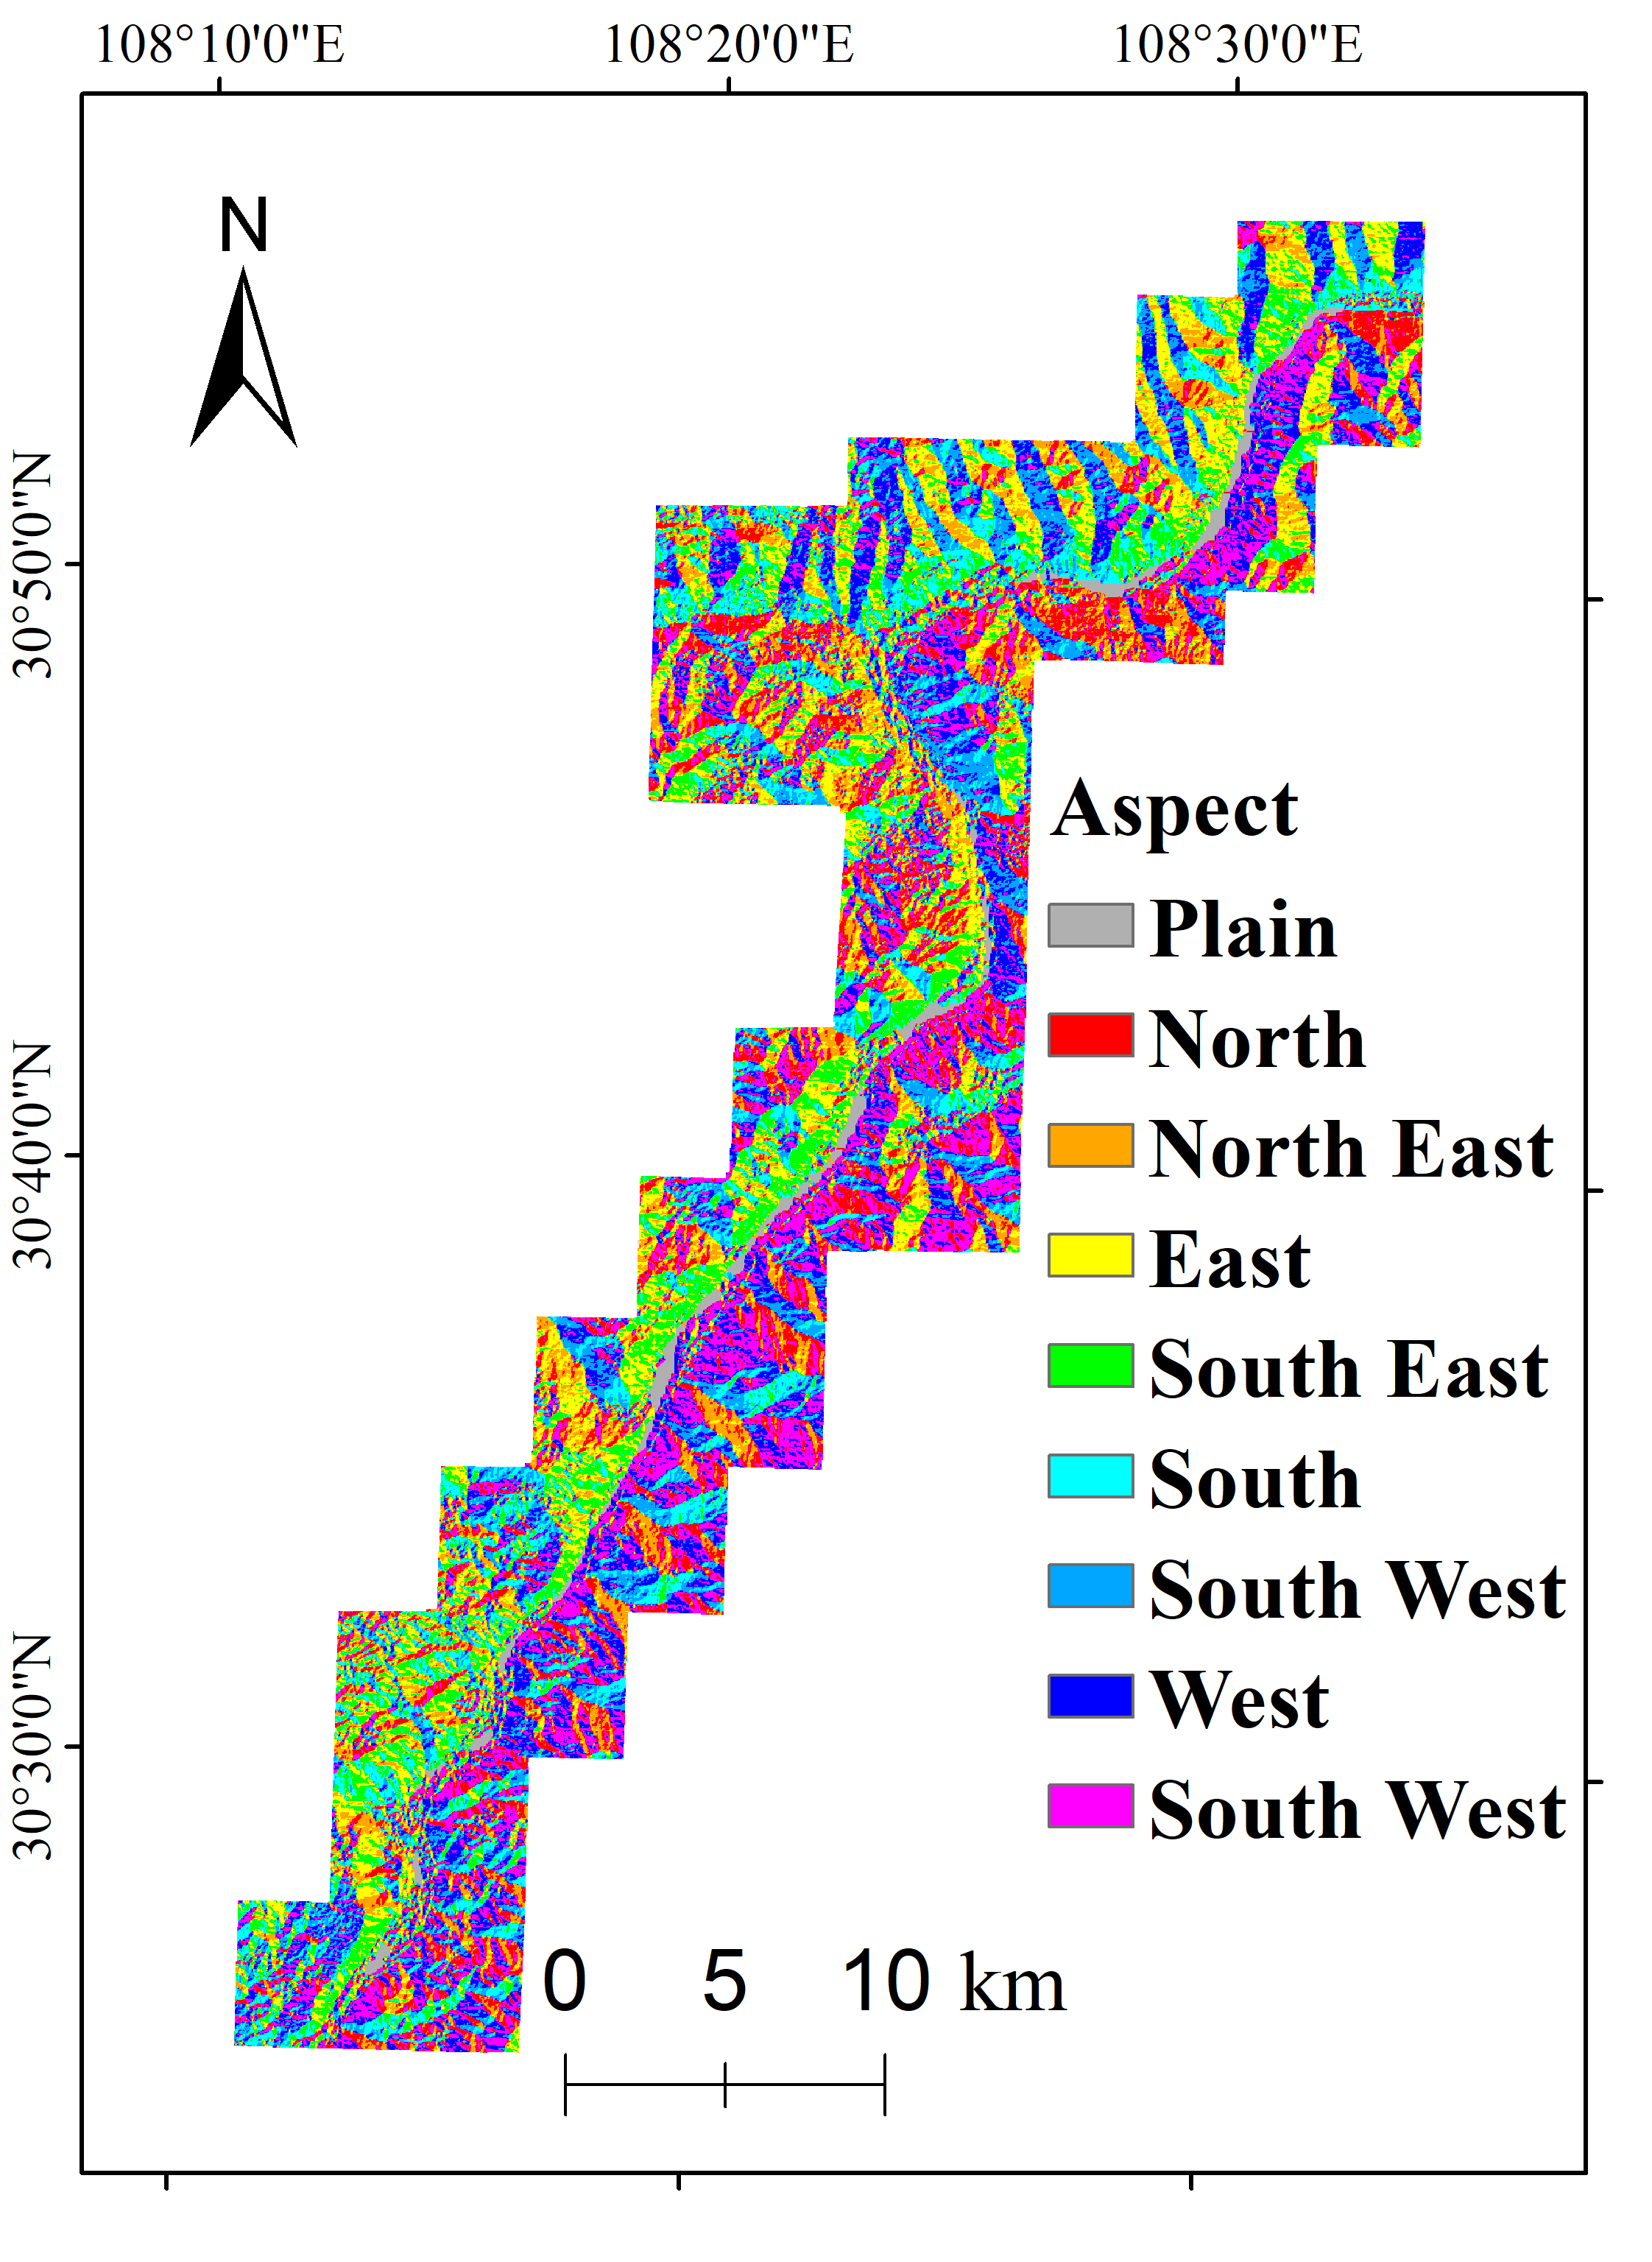
\includegraphics[width=4.5cm]{Definitions/Aspect.png}
    }
    \quad
    \subfigure[~Curvature]{
    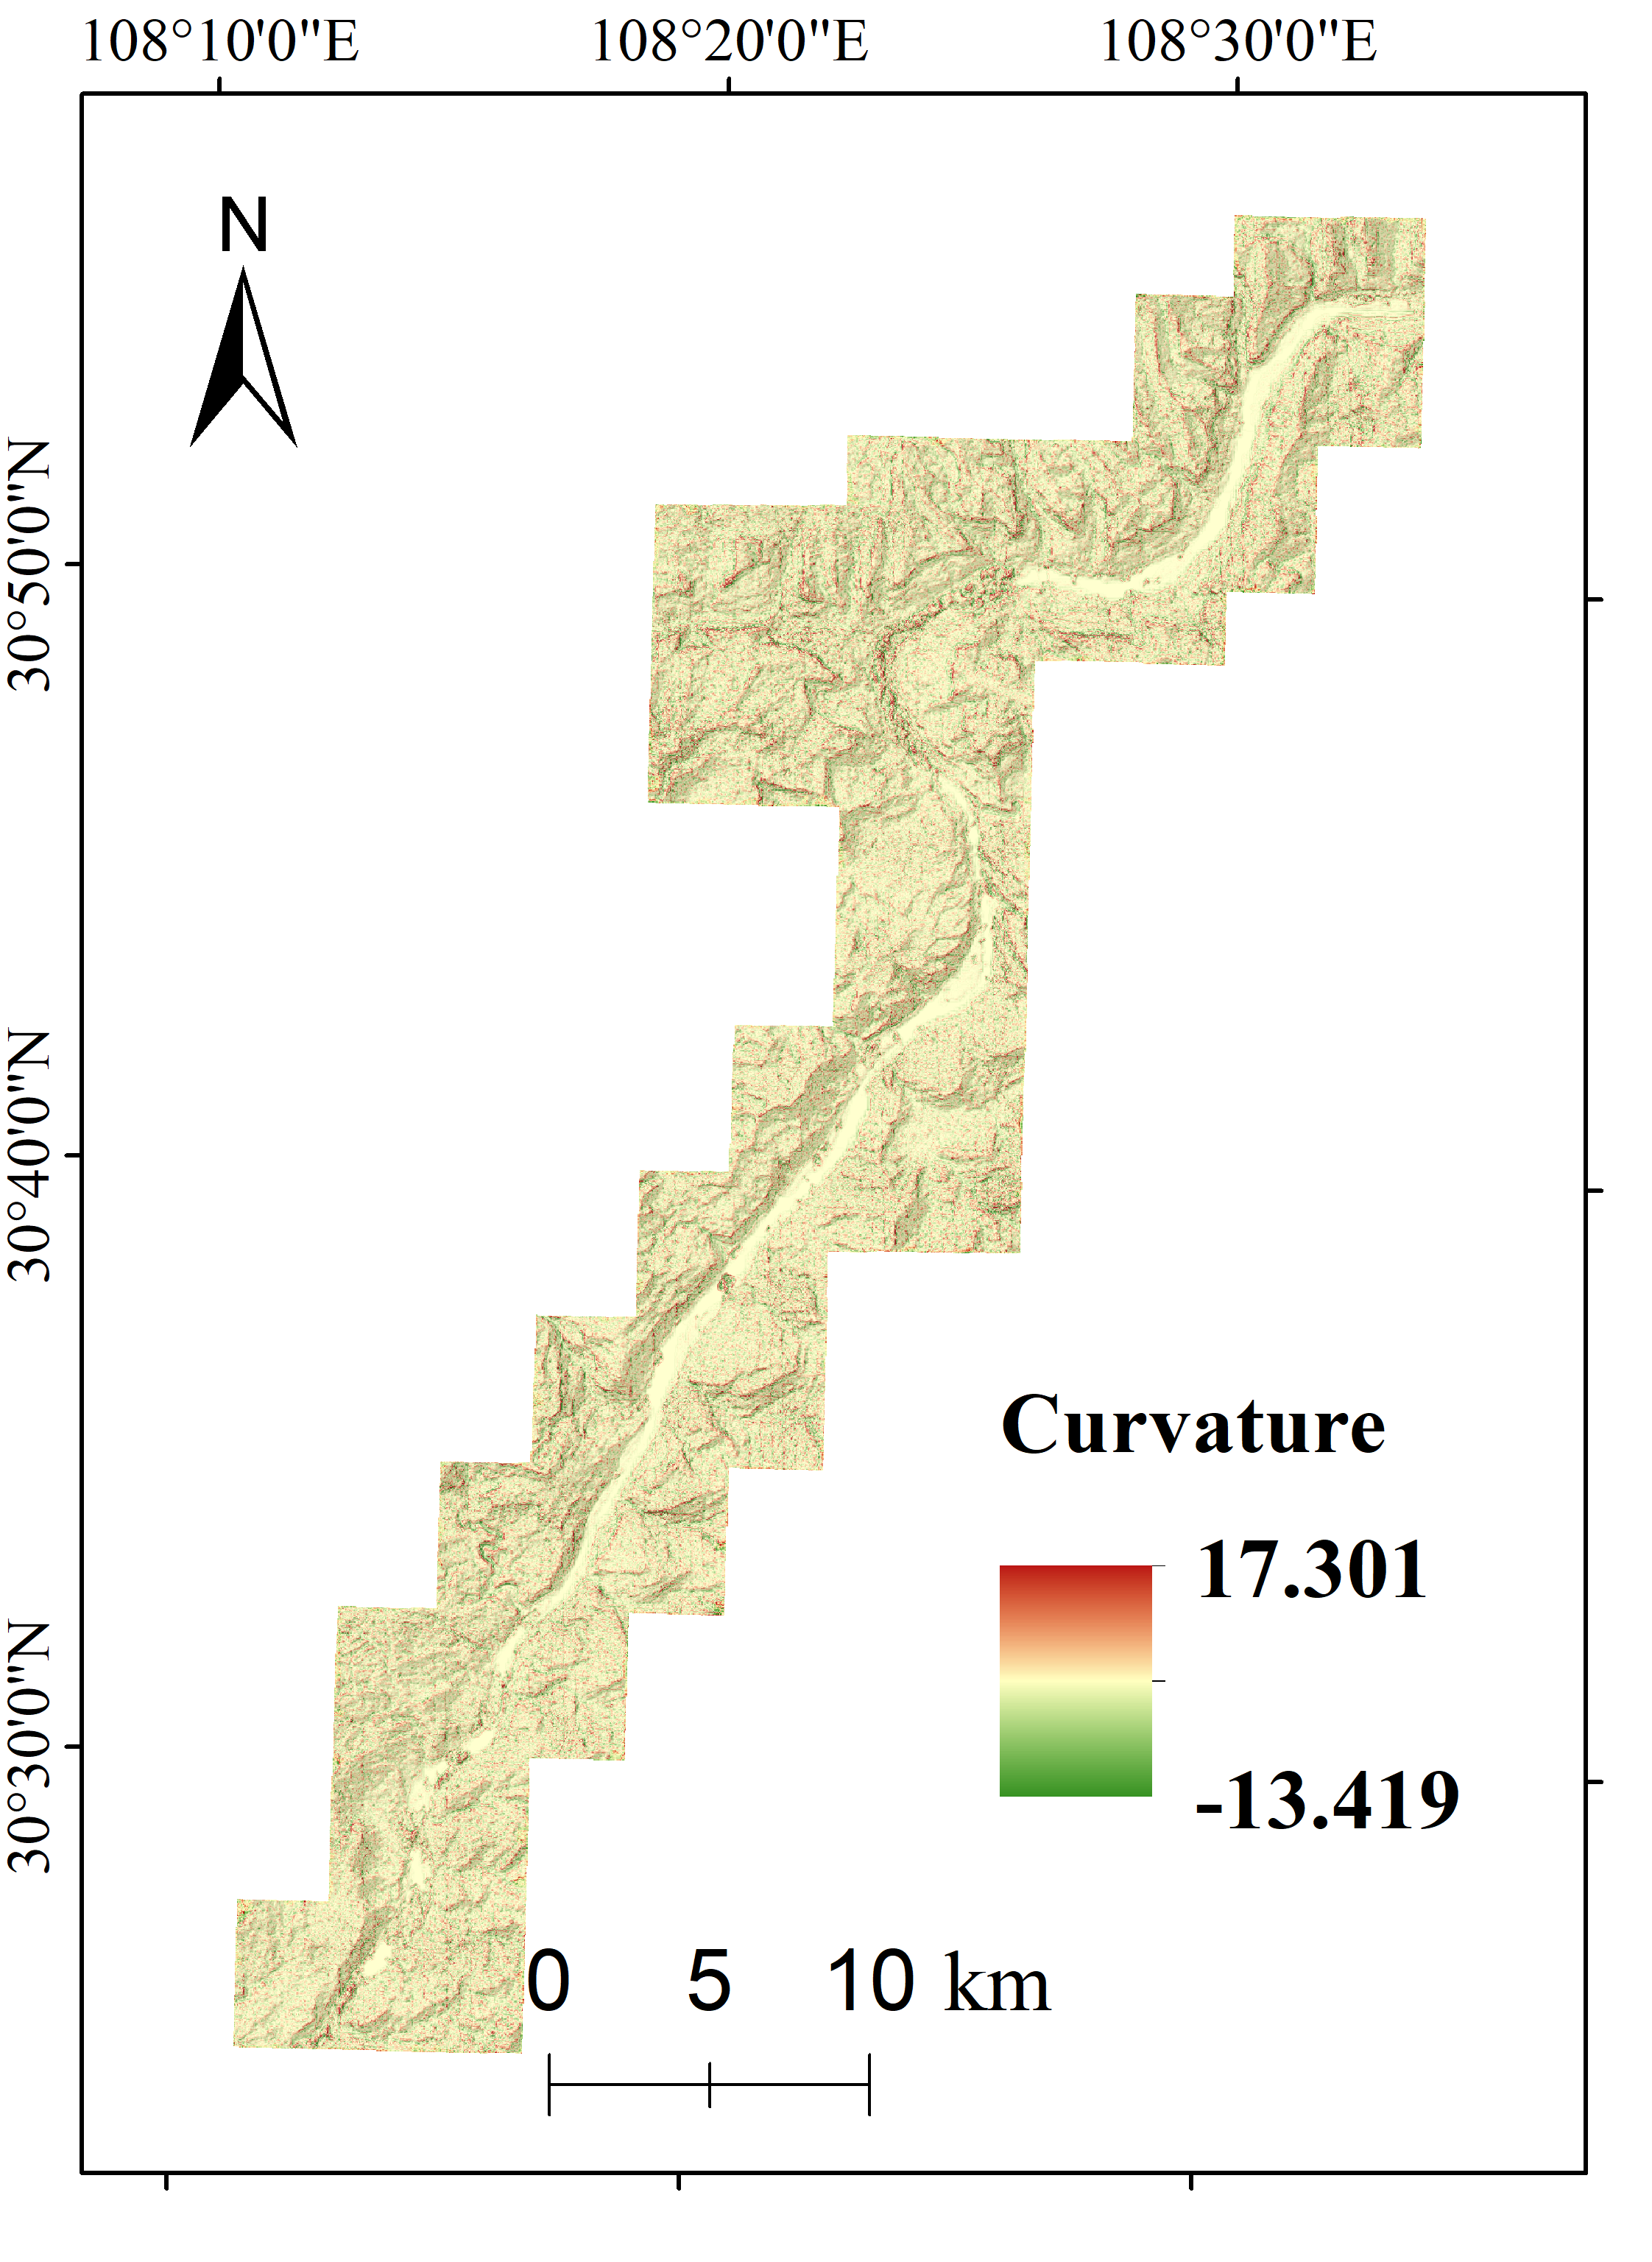
\includegraphics[width=4.5cm]{Definitions/Curvature.png}
    }
    \quad
    \subfigure[~Distance to river]{
    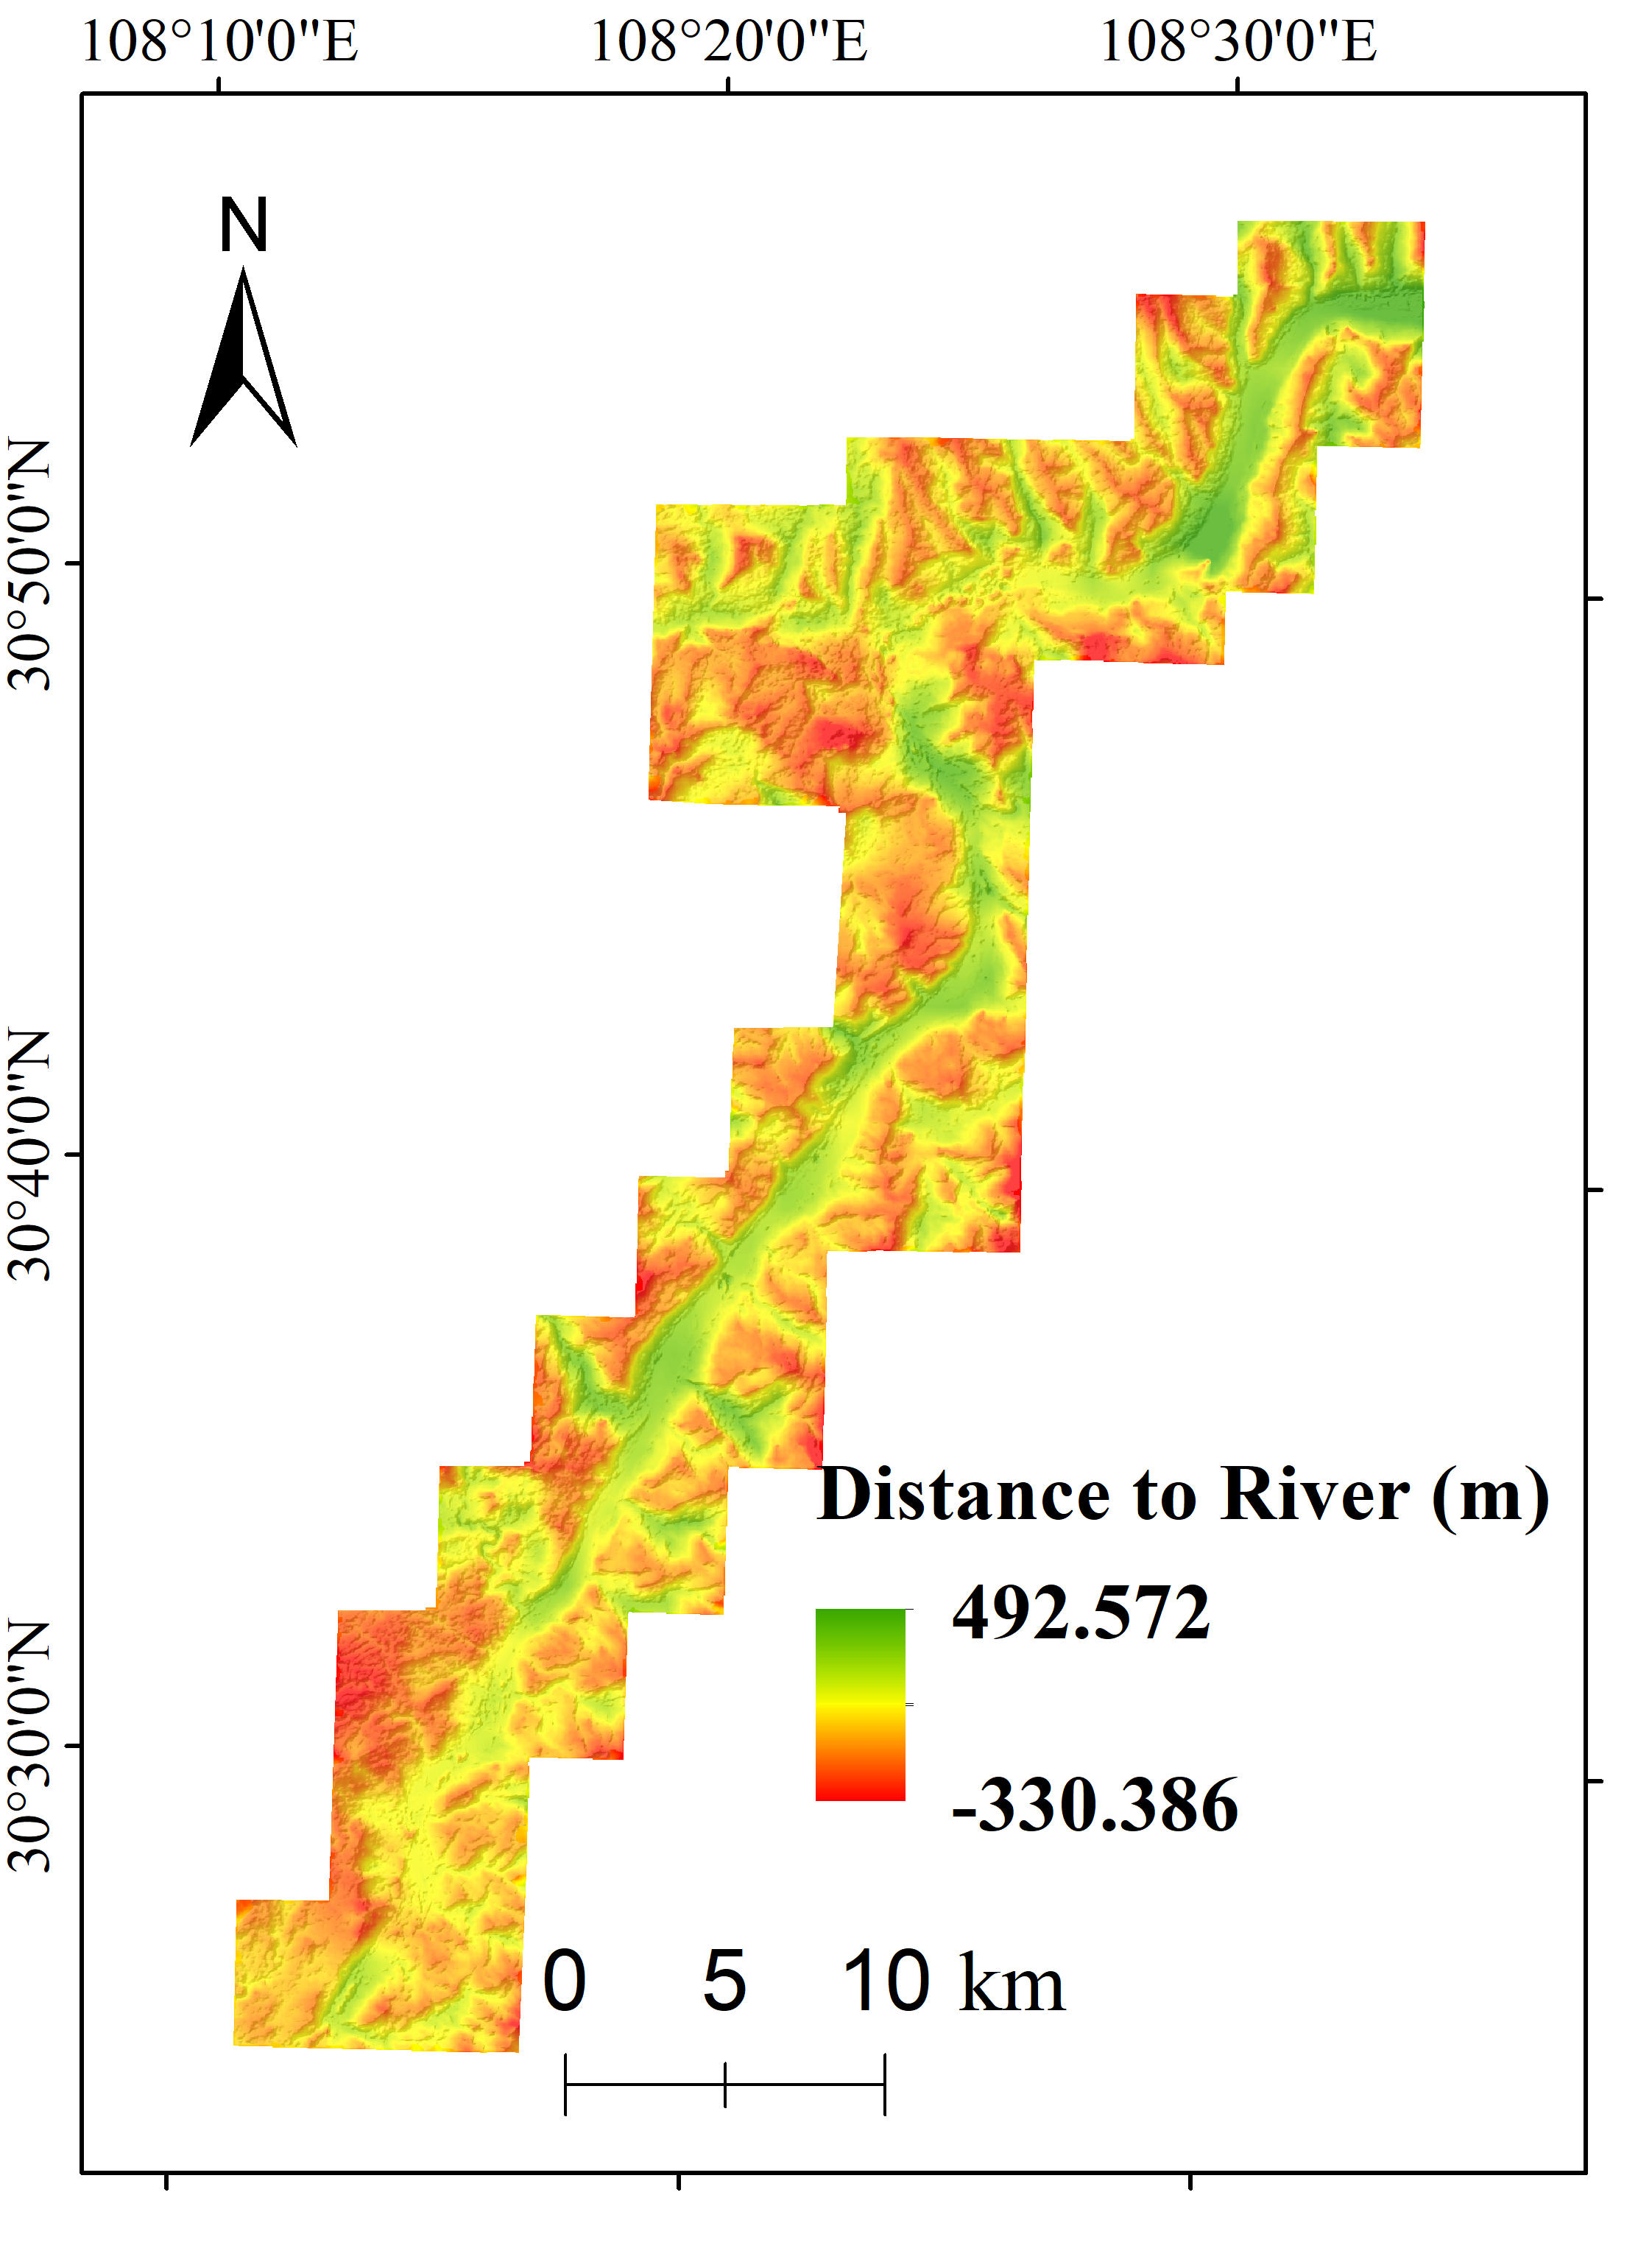
\includegraphics[width=4.5cm]{Definitions/DistanceToRiver.png}
    }
    \quad
    \subfigure[~NDVI]{
    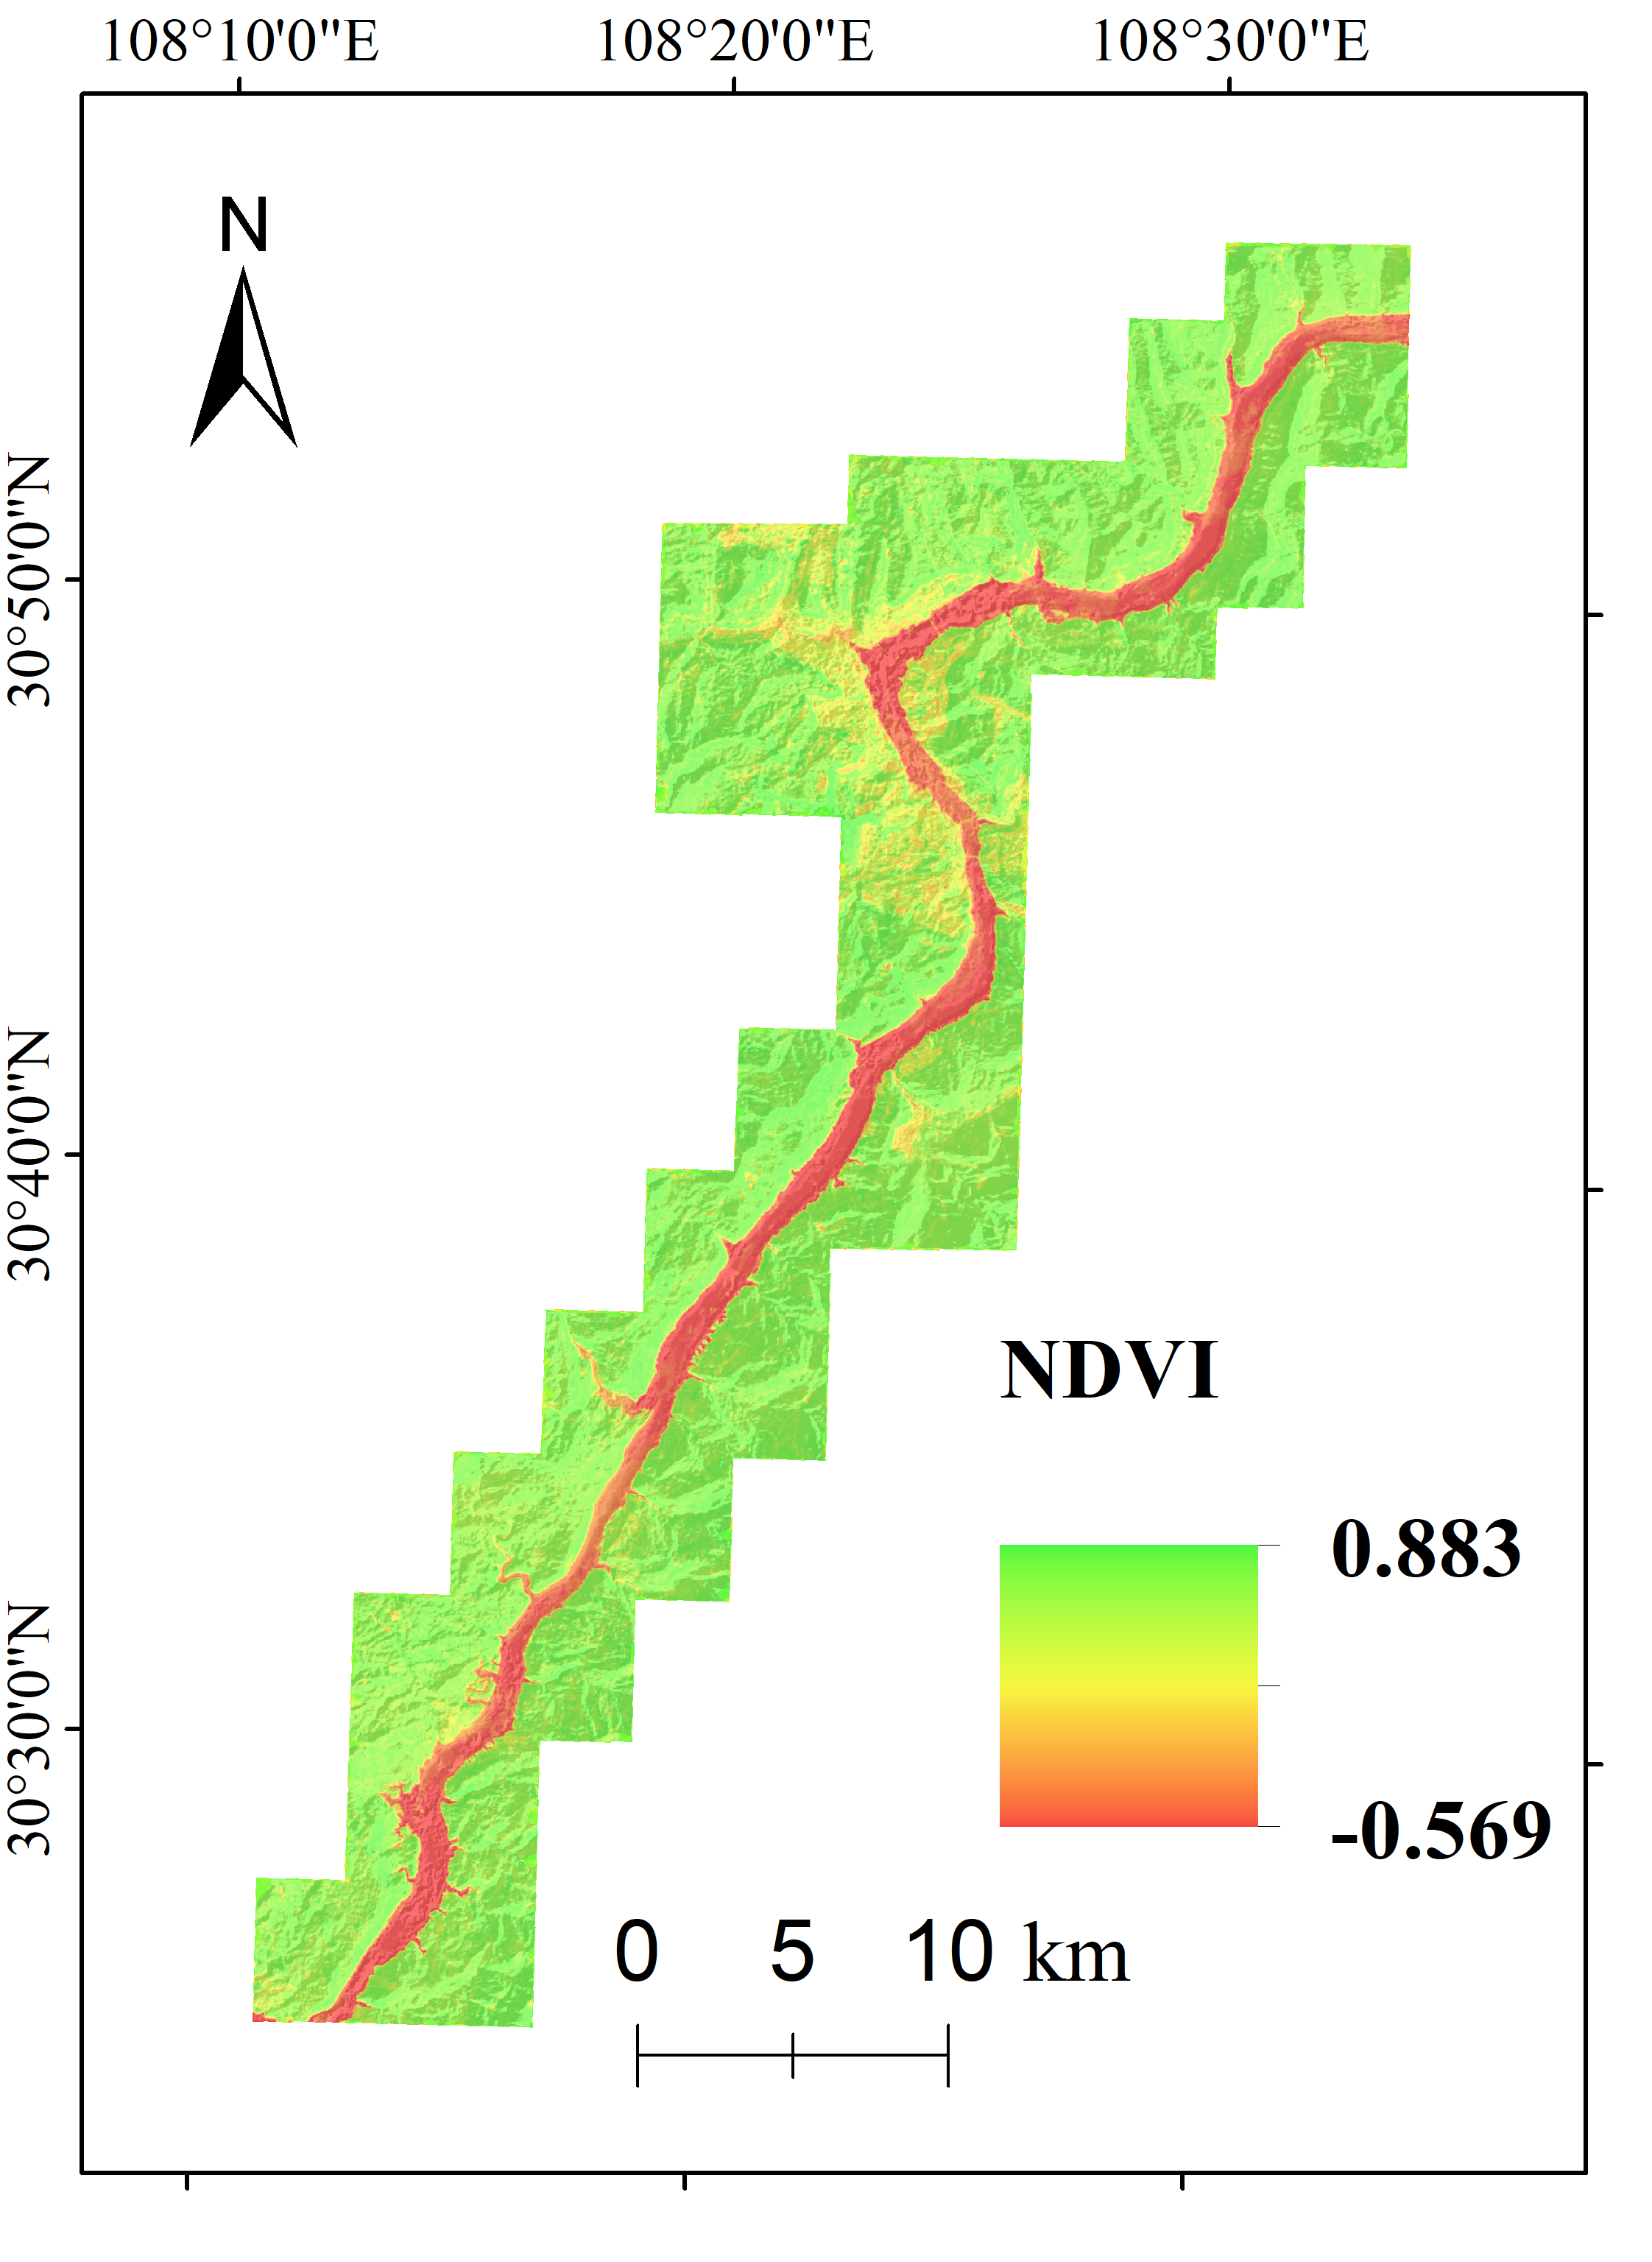
\includegraphics[width=4.5cm]{Definitions/NDVI.png}
    }
  \end{figure}
  \addtocounter{figure}{0} % 将图的编号减0
  \begin{figure}
  \centering
  \addtocounter{subfigure}{0} % 子图编号加0
    \subfigure[~NDWI]{
    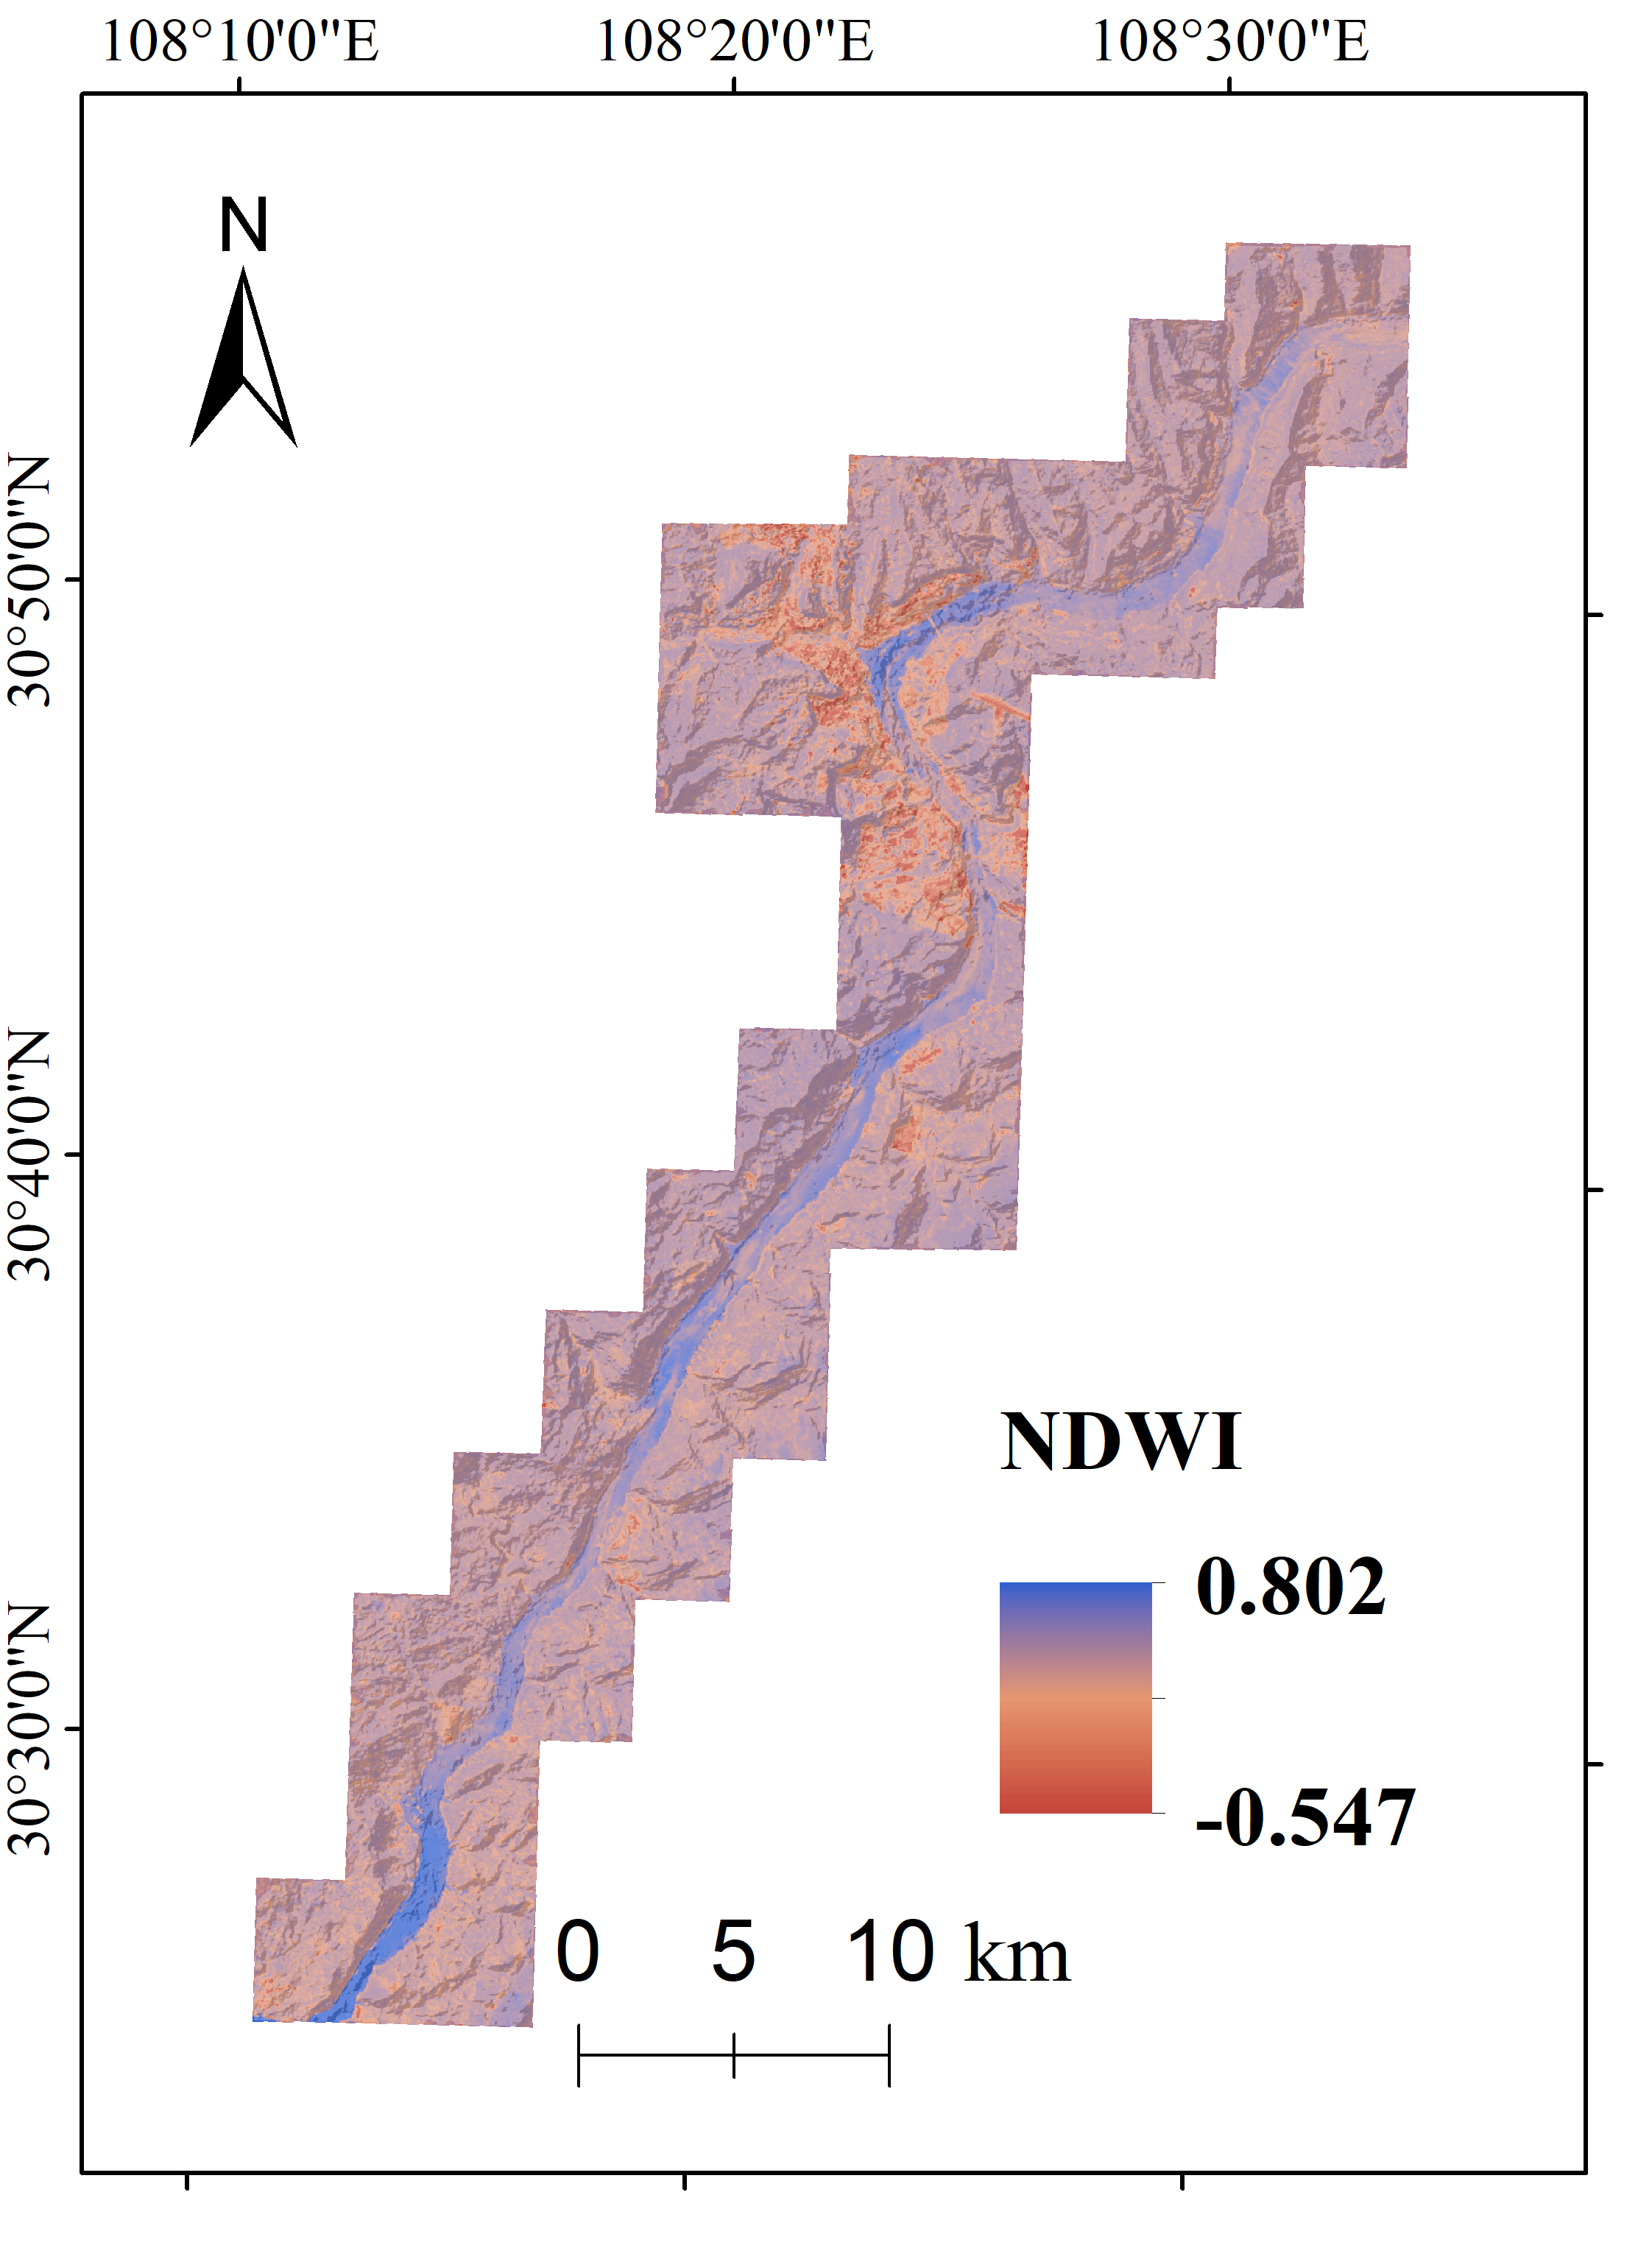
\includegraphics[width=4.5cm]{Definitions/NDWI.png}
    }
    \quad
    \subfigure[~Rainfall]{
    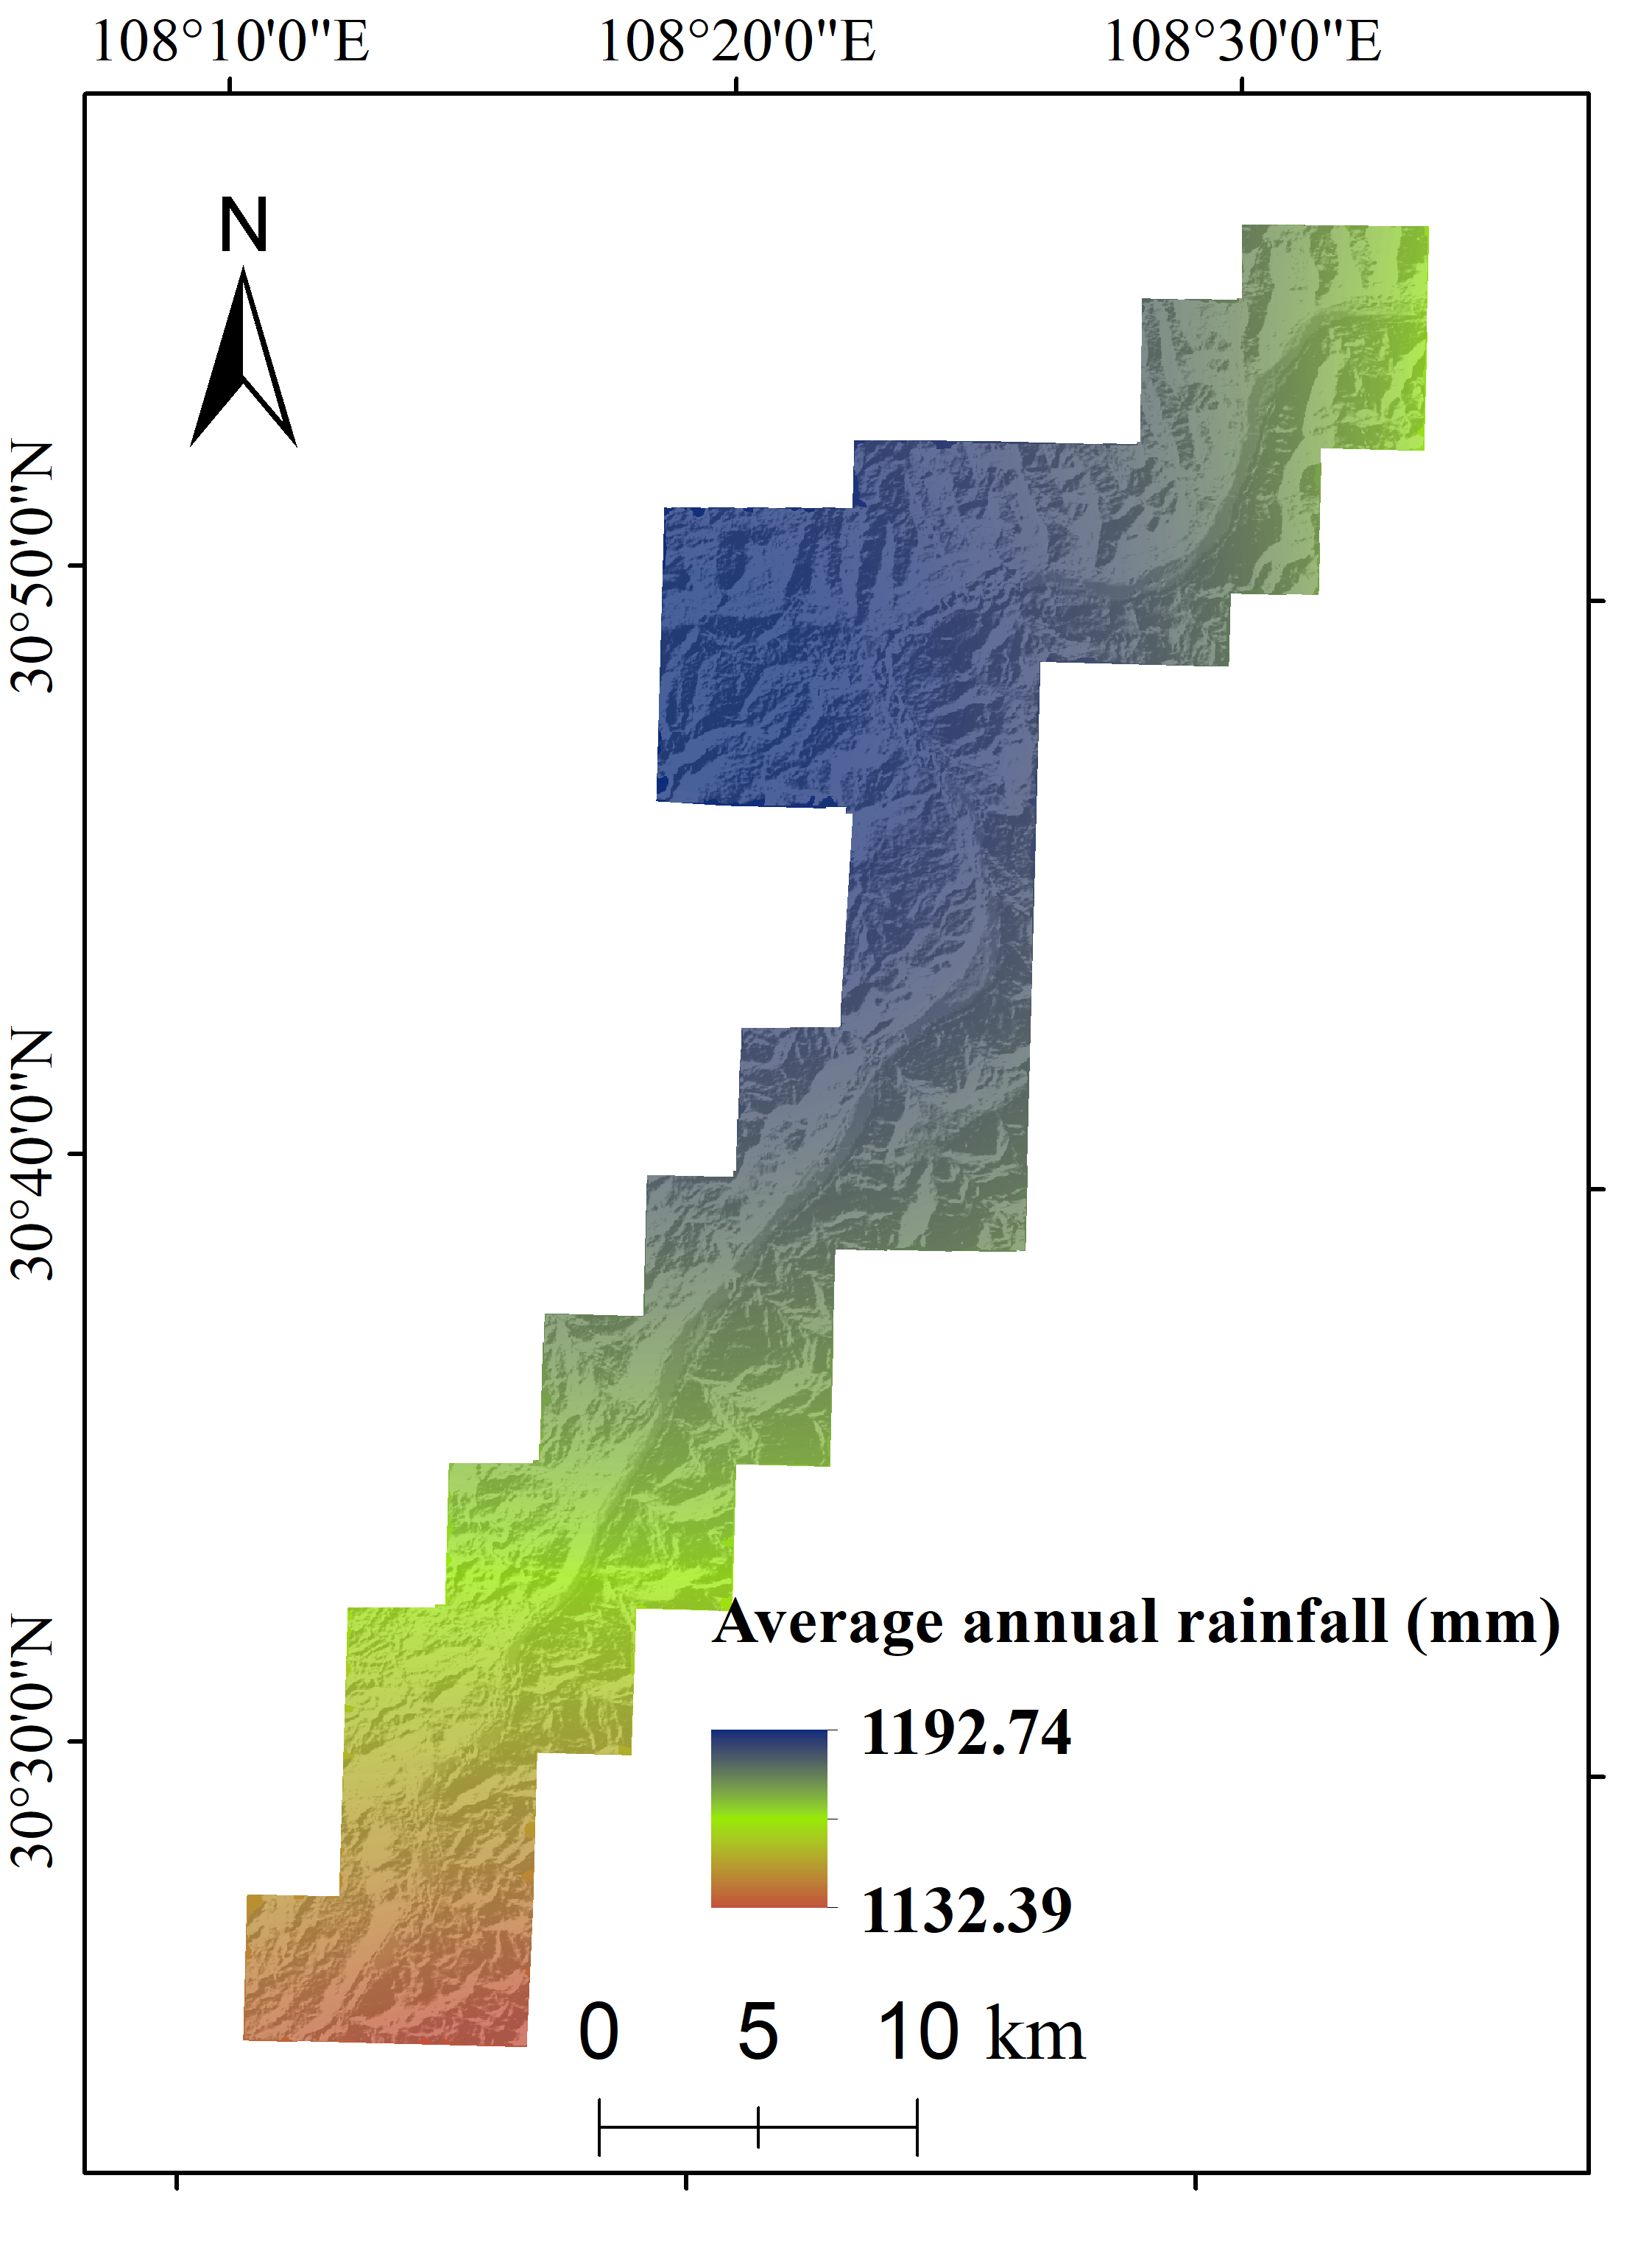
\includegraphics[width=4.5cm]{Definitions/Rain.png}
    }
    \quad
    \subfigure[~Seismic intensity]{
    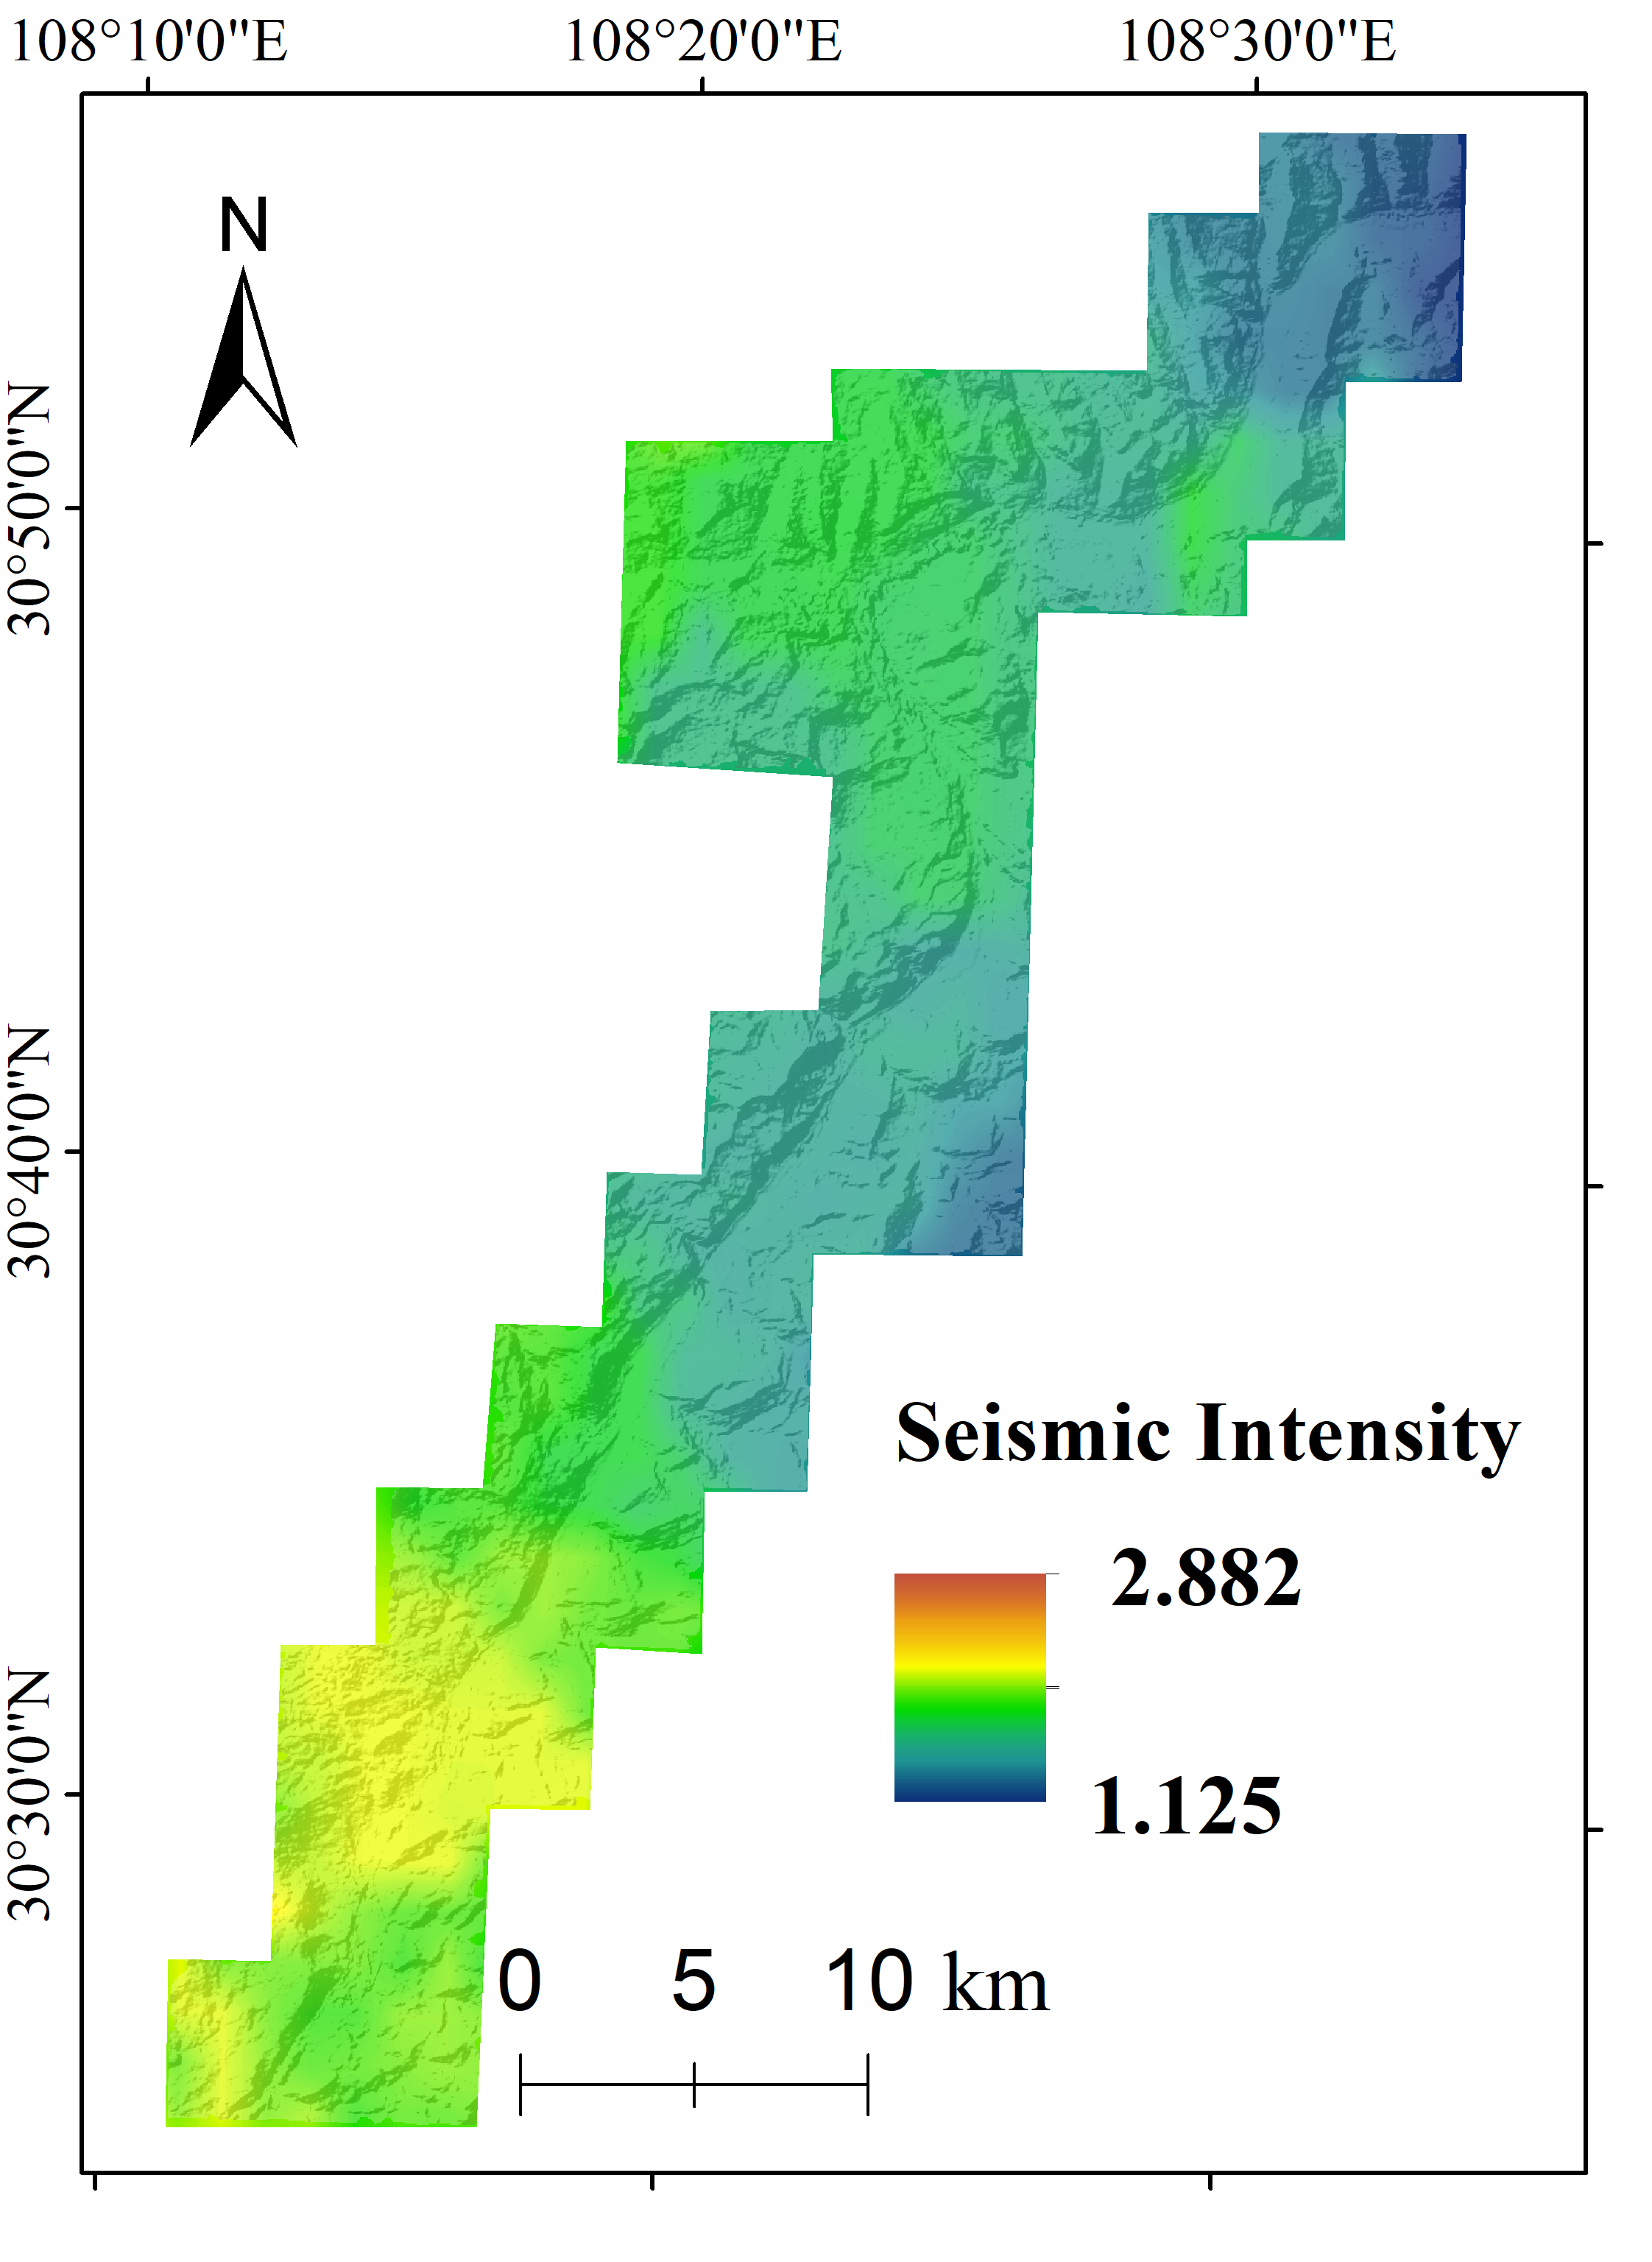
\includegraphics[width=4.5cm]{Definitions/intensity.png}
    }
    \quad
    \subfigure[~Landuse]{
    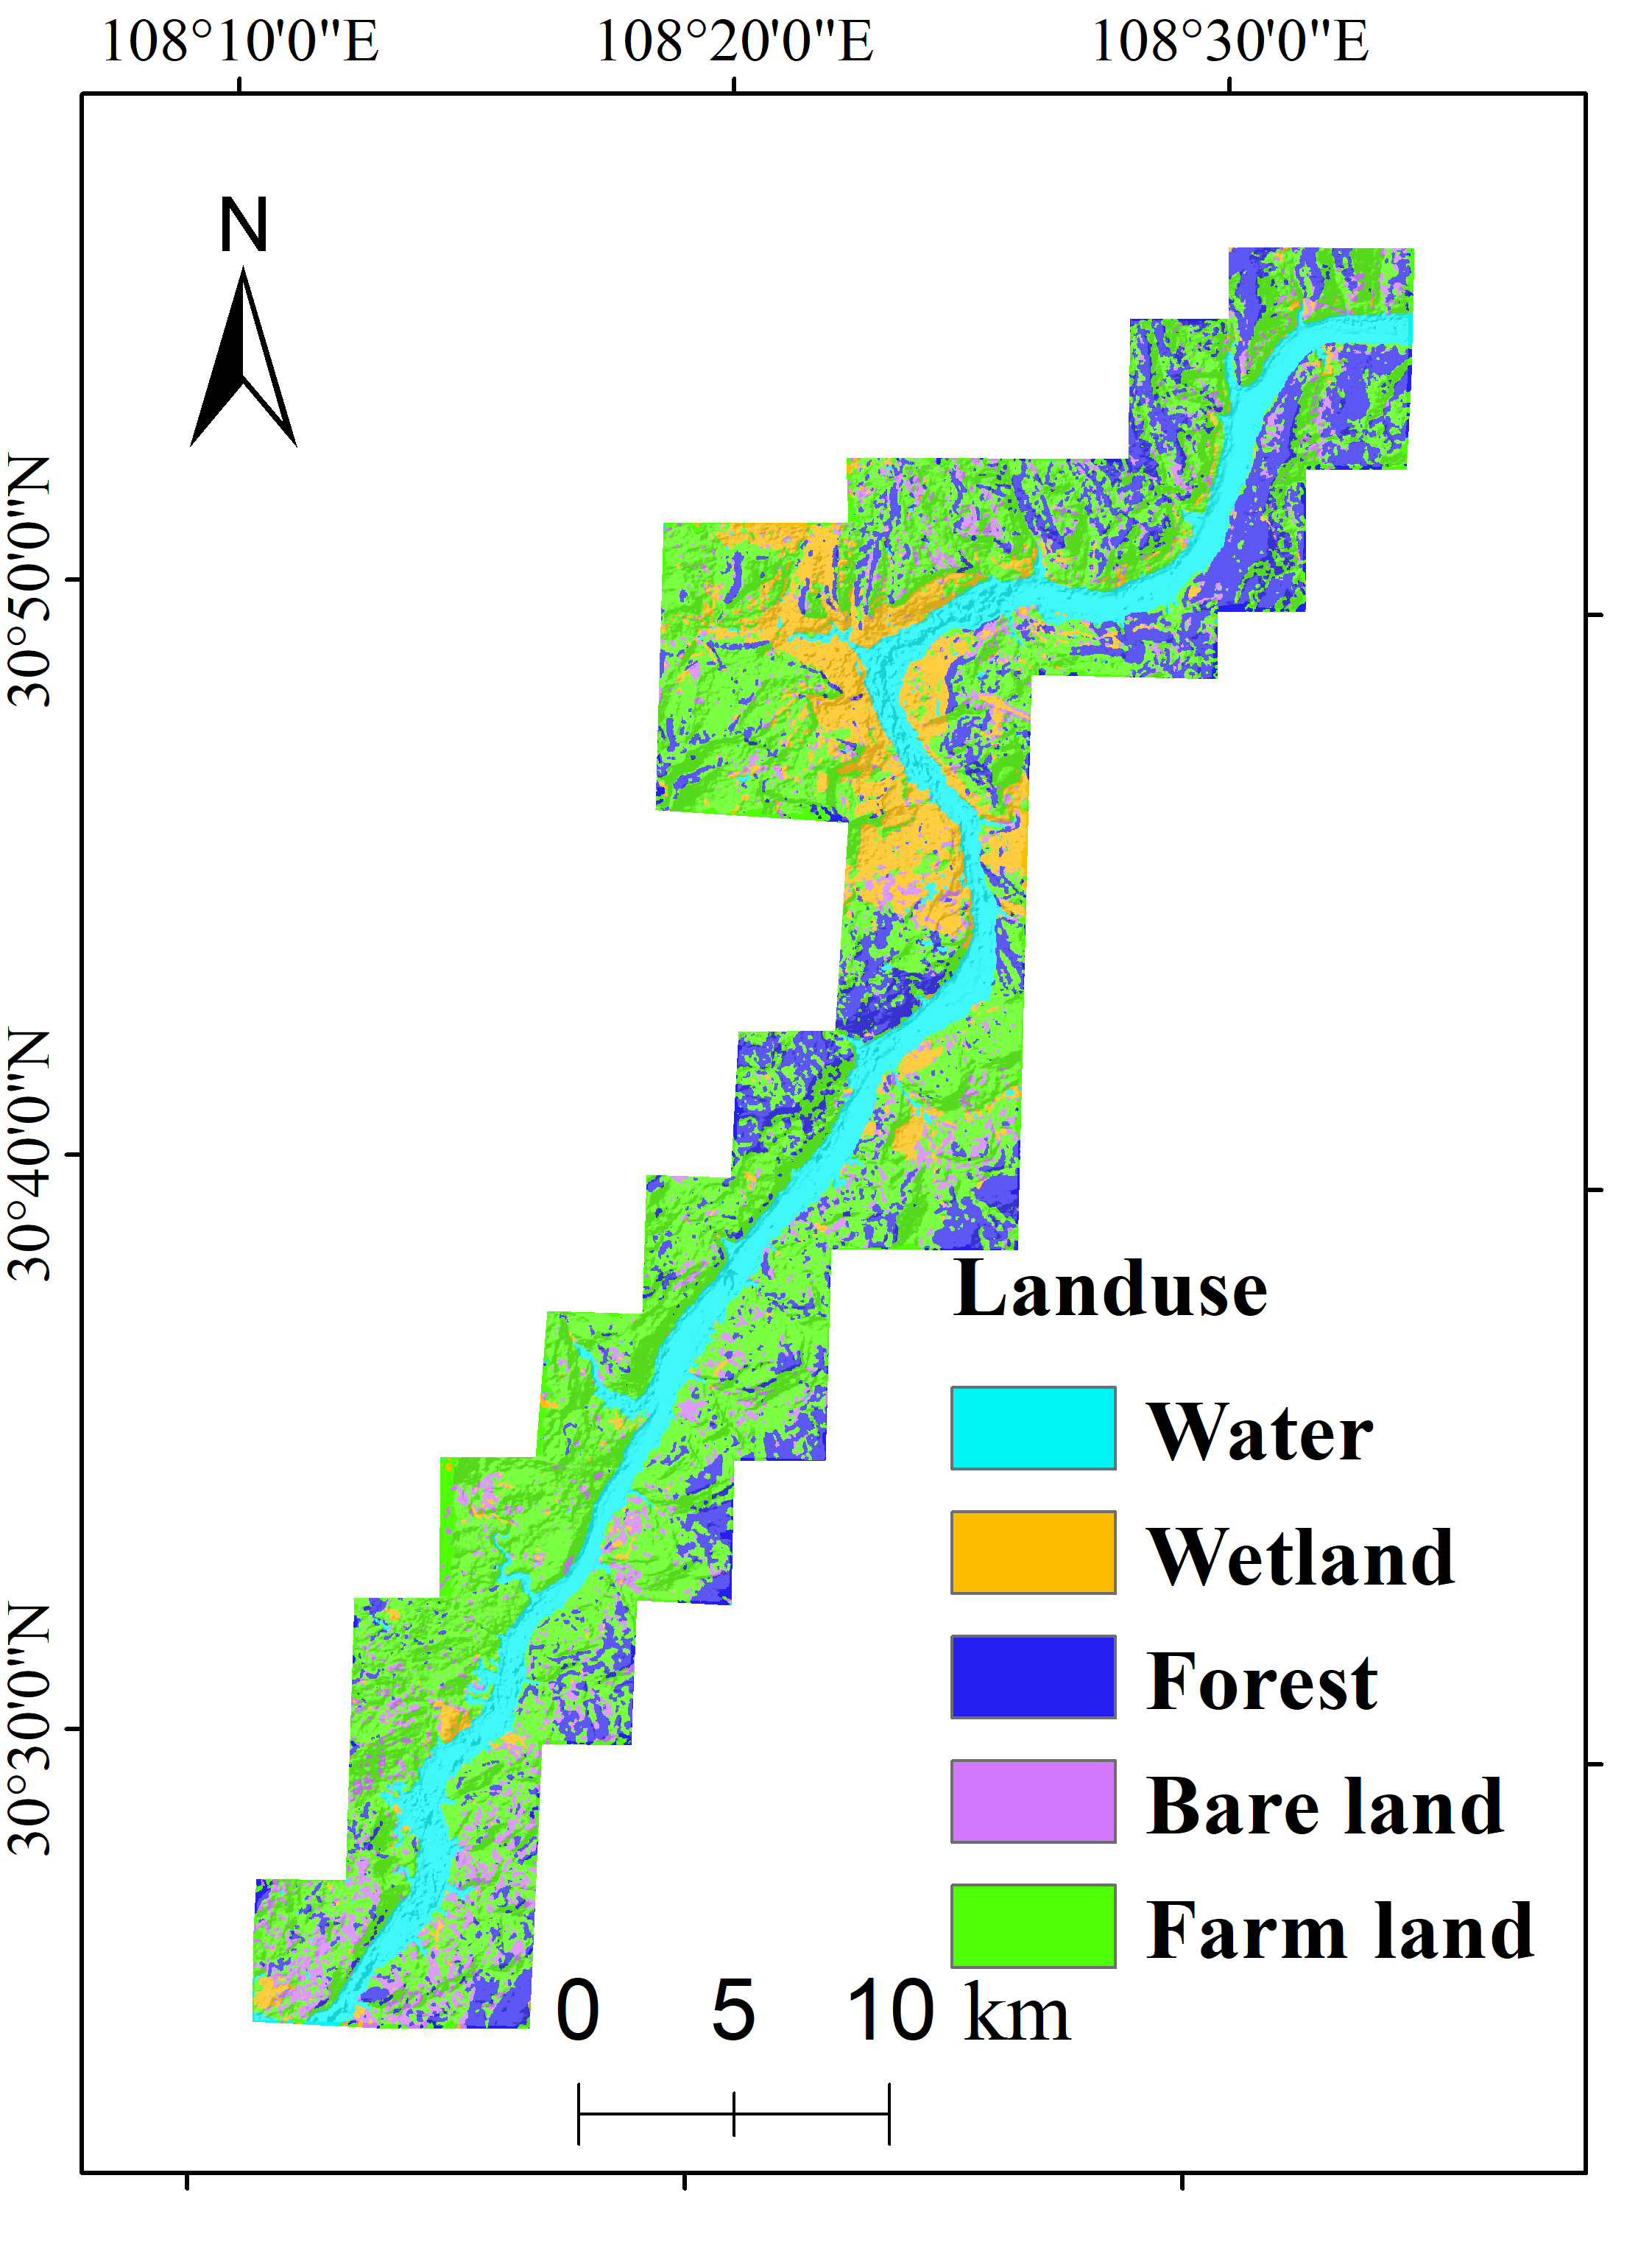
\includegraphics[width=4.5cm]{Definitions/Landuse.png}
    }
    \quad
    \subfigure[~TRI]{
    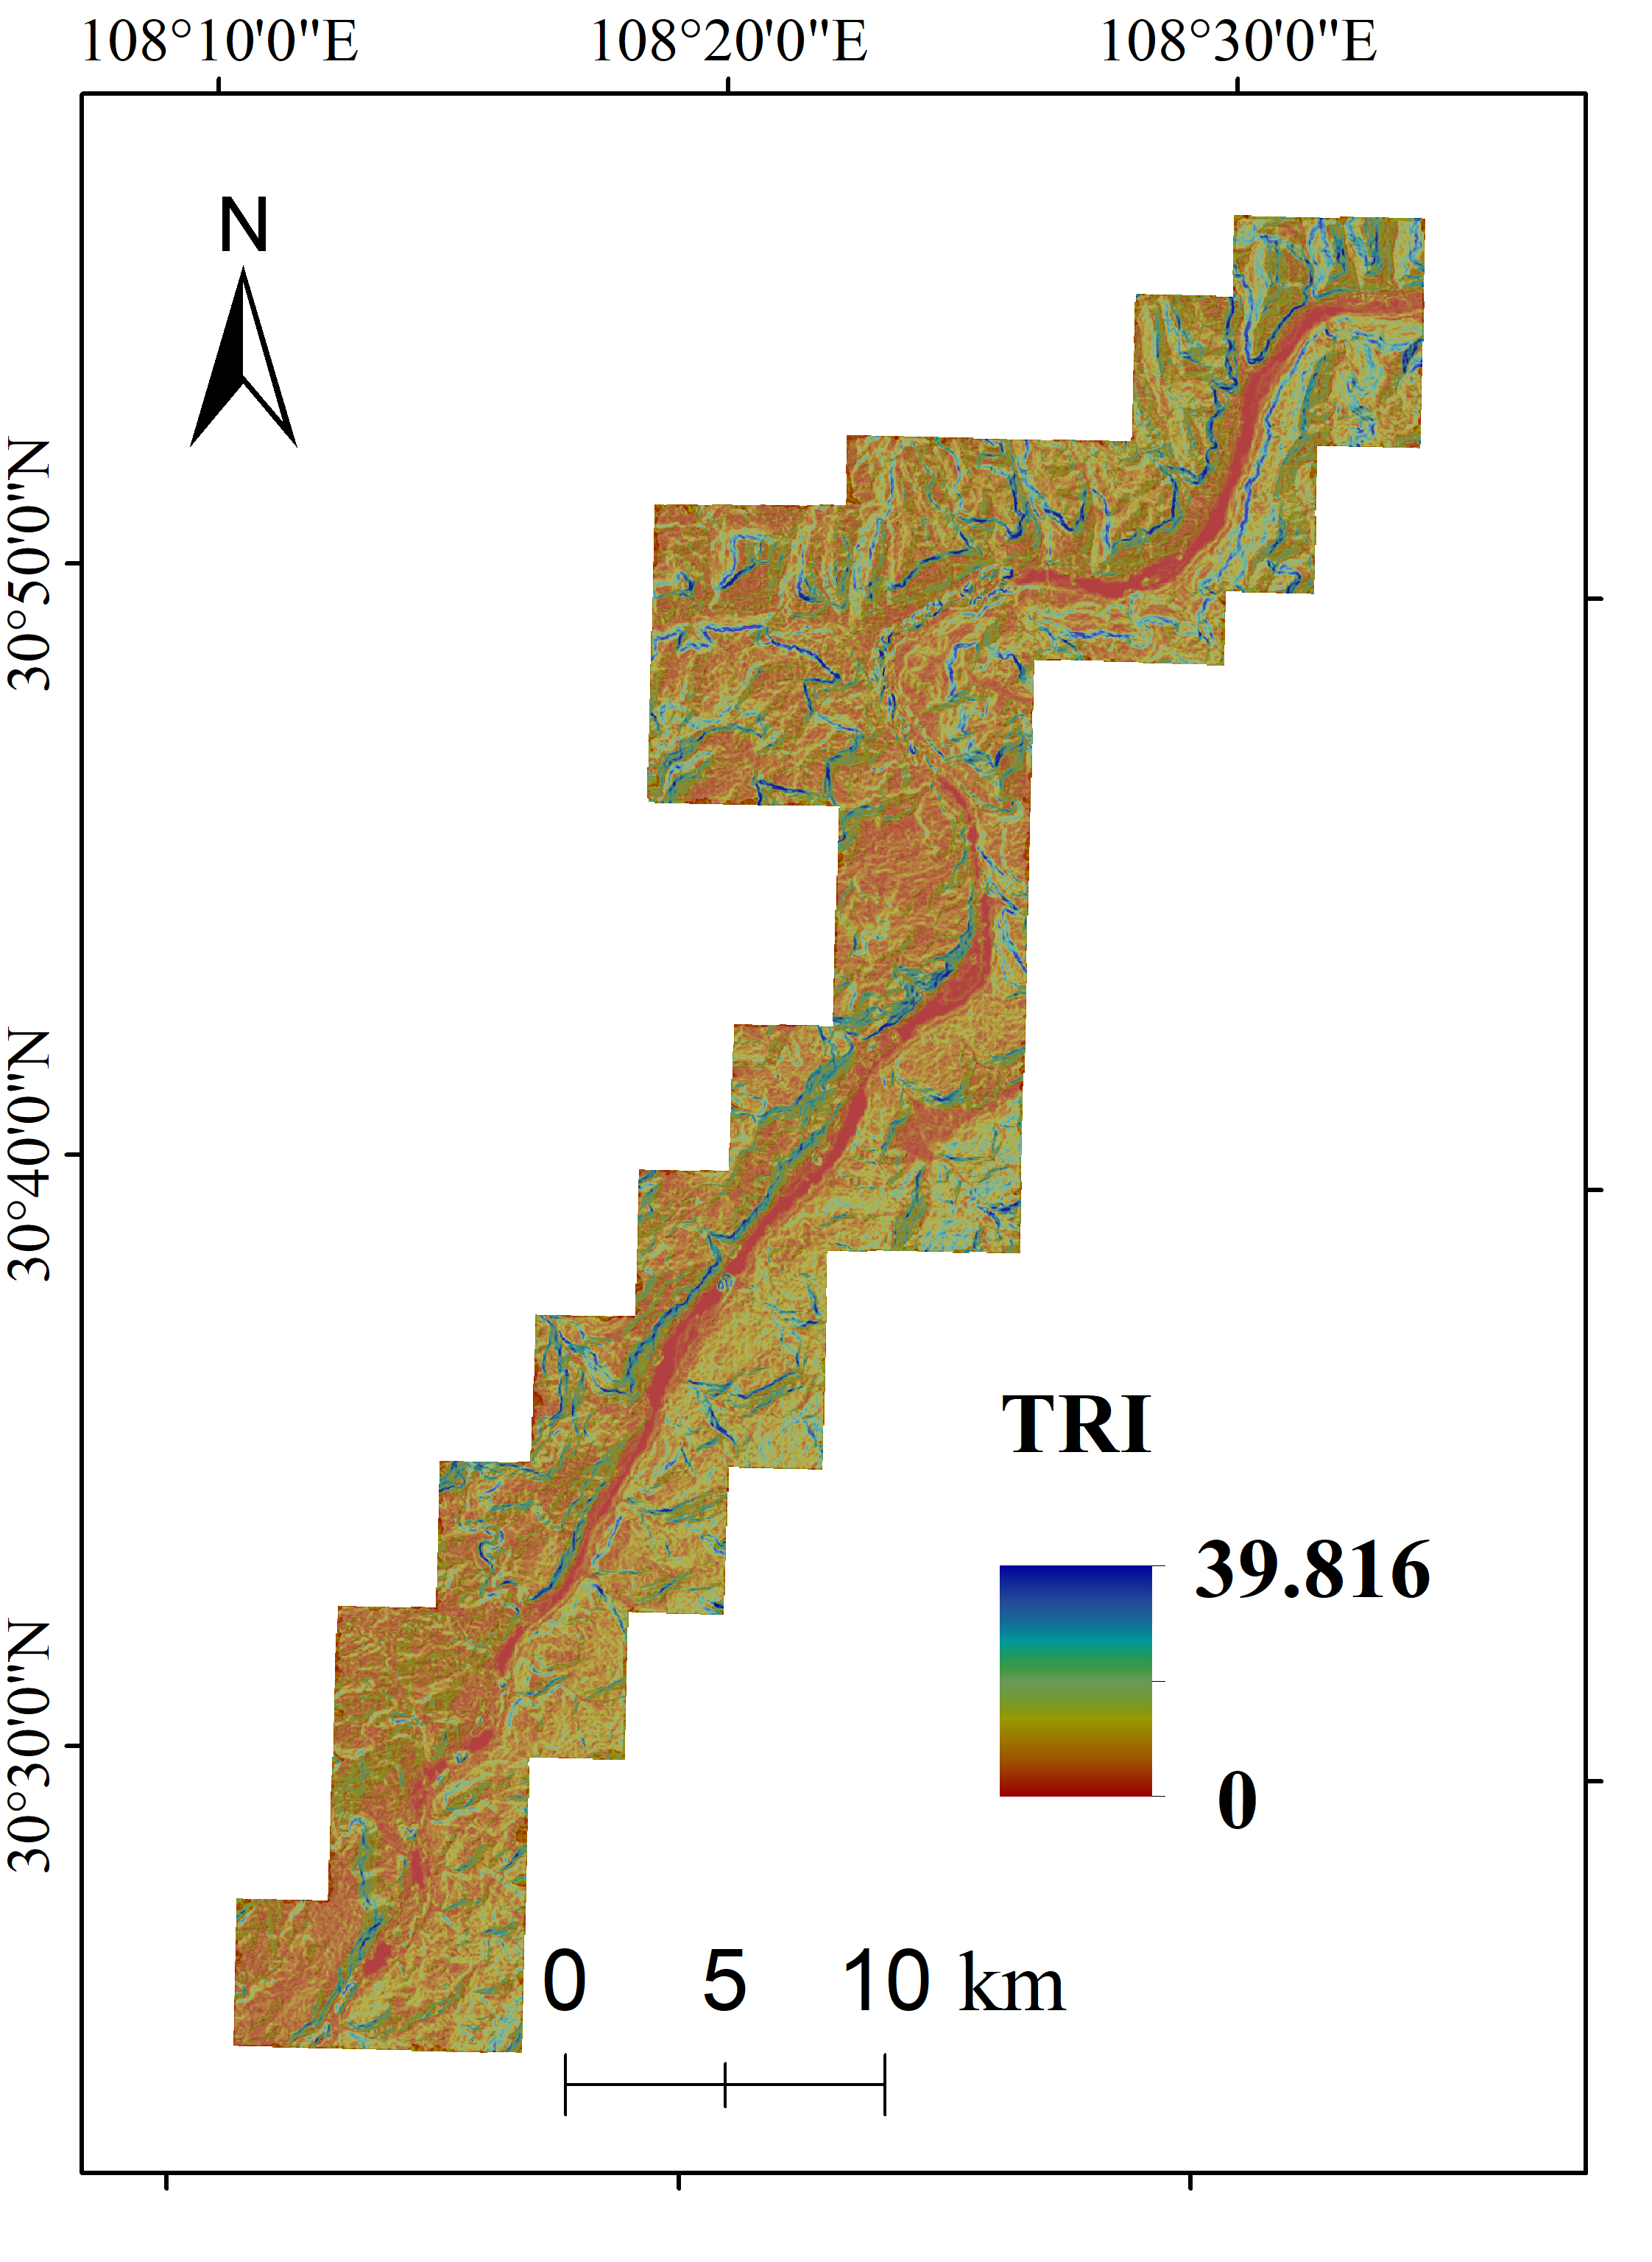
\includegraphics[width=4.5cm]{Definitions/TRI.png}
    }
    \quad
    \subfigure[~Lithology]{
    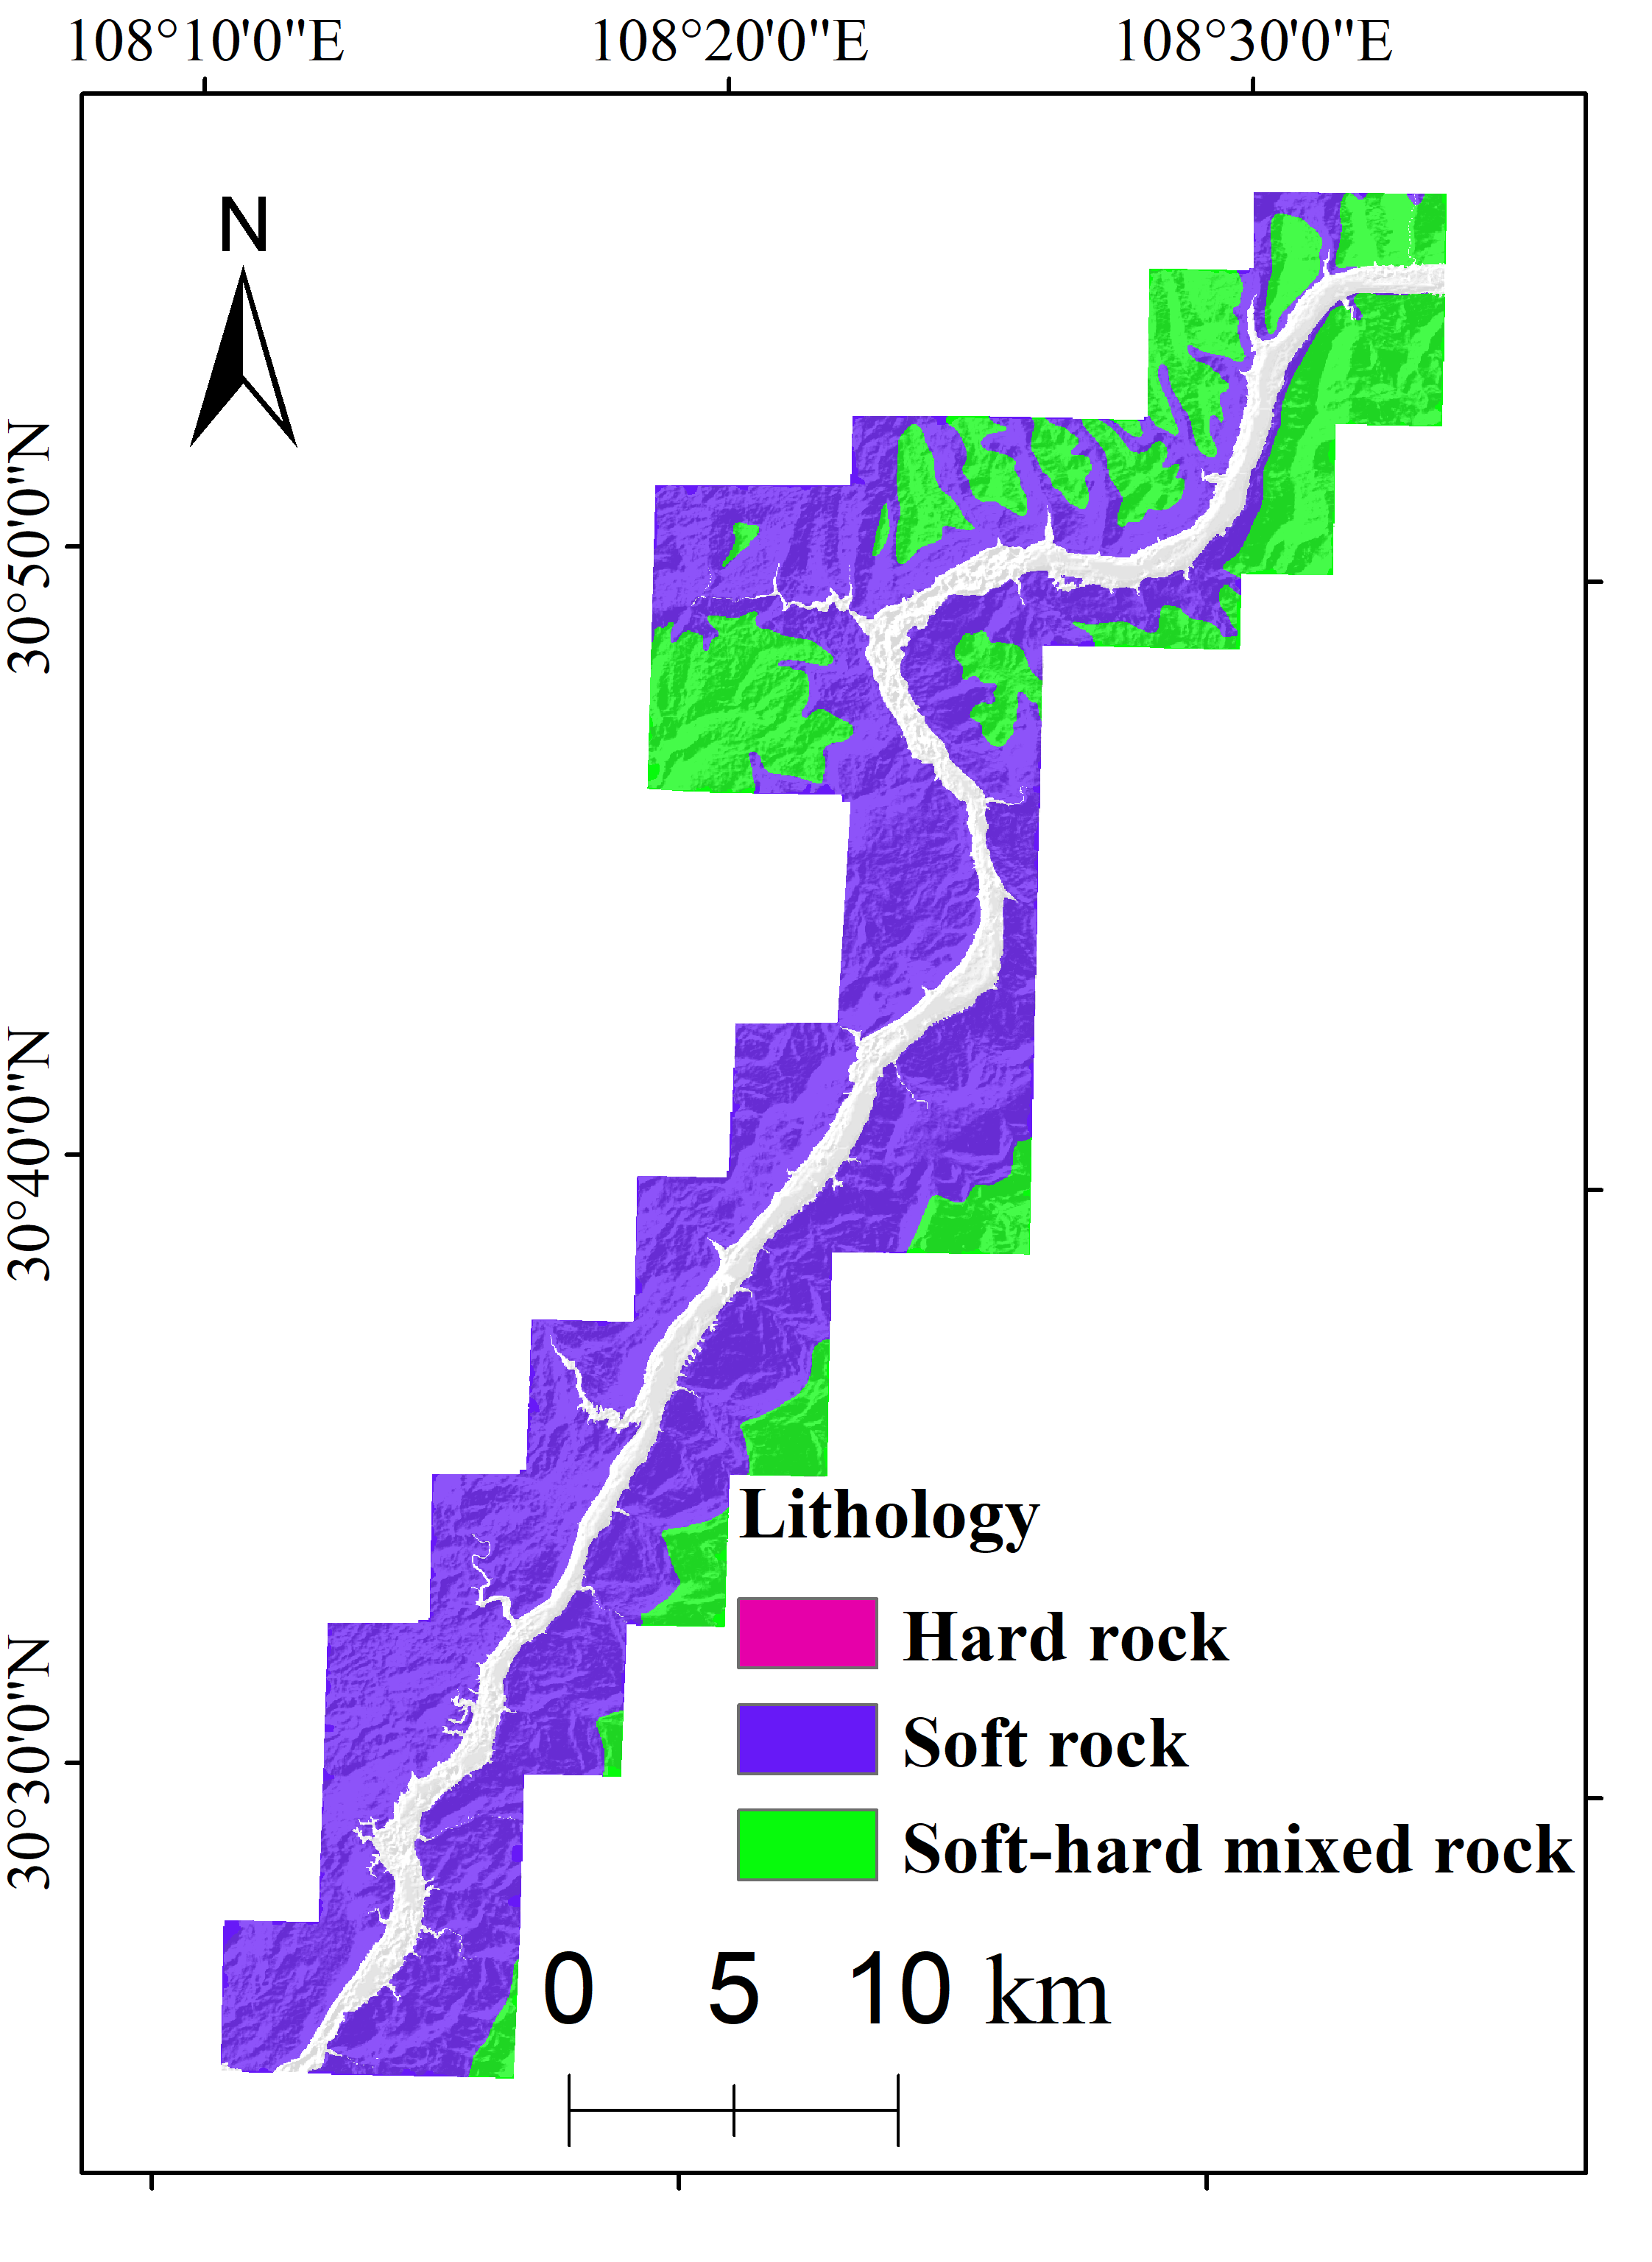
\includegraphics[width=4.5cm]{Definitions/rock.png}
    }
    \caption{Landslide factors used in the study.(\textbf{a}) Elevation.(\textbf{b}) Slope.(\textbf{c}) Aspect.(\textbf{d}) Curvature.(\textbf{e}) Distance to the river (m).(\textbf{f}) NDVI.(\textbf{g}) NDWI.(\textbf{h}) Rainfall. (\textbf{i}) Seismic intensity. (\textbf{j}) Landuse. (\textbf{k}) TRI. (\textbf{l}) Lithology.}
    \label{Fig_Landslide_Factors}
\end{figure}

\section{Methodology}

The flowchart of landslide susceptibility mappingfor the study area is shown as in Fig. \ref{LSM4RS_FlowChart}. 

\begin{figure}
  \centering
  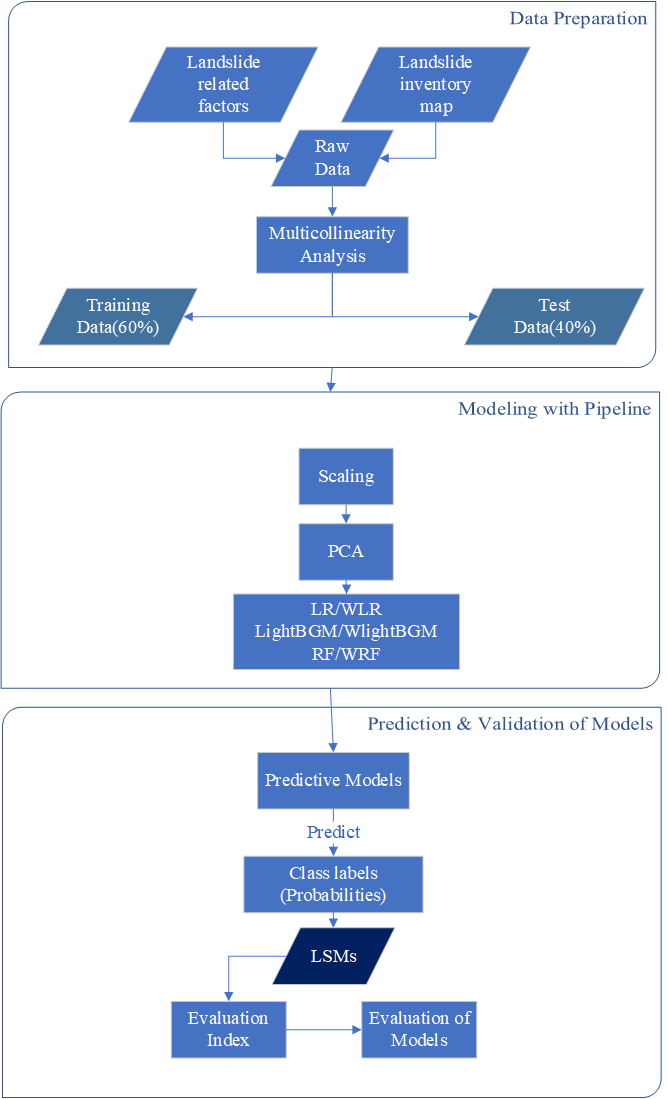
\includegraphics[width=10 cm]{Definitions/Workflow.png}
  \caption{Overall workflow of this study.}
  \label{LSM4RS_FlowChart}
\end{figure}

Firstly, twelve landslide contributing factors and landslide samples were selected as independent variables and dependent variables, respectively, to form an initial decision table for training the models. 
Not all the landslide contributing factors are indispensable for the landslide susceptibility assessment (Dou et al., 2015). 
Therefore, multicollinearity analysis of landslide contributing factors is essential for improving the robustness of the models. 
In this study, the variance inflation factor method (VIF) was utilized to carry out multicollinearity analysis of landslide conditioning factors. 
Secondly, a so-called "Pipeline" strategy was used to connect data processing and classifiers. 
The disposing of data includes factor-normalization and factor-reduction in which the StandardScaler function and PCA method provided by Sklearn were implemented (Pedregosa et al., 2011). 
The purpose of employing "Pipeline" is to ensure the consistency of the data preprocessing in the training set and test set. 
Thirdly, the traditional machine learning (logistic regression) and ensemble machine learning models (LightGBM and random forest) were applied to achieve the landslide susceptibility mapping. 
Finally, several evaluation indicators (e.g., AUC value, balanced accuracy, and geometric mean score) were implemented to evaluate the LSM models.


\subsection{Logistic Regression (LR)}

Logistic regression (LR) is a classic machine learning model with the capacity to settle classification problems \citep{Ayalew2005Geomorphology,Bai2010Geomorphology,Song2018}. 
It is widely used in landslide susceptibility evaluation because of its simplicity, parallelization, and strong interpretability. 
Logistic regression can be treated as a variant of linear regression, and the variables of the LR model could be continuous or discrete \citep{Ayalew2005Geomorphology,Bai2010Geomorphology}. 
The core concept of logistic regression is to map the domain's value from (-$\infty$, +$\infty$) to (0,1). 
0 and 1 represent different categories, respectively. 
They represent non-landslides (0) and landslides (1) in the landslide susceptibility evaluation. 
A Sigmoid function is employed to express this mapping relationship, as shown below (Equation \ref{eqn:gz}).

\begin{equation}
  g(z)=\frac{1}{1+e^{-z}}
  \label{eqn:gz}
\end{equation}

\subsection{LightGBM}

LightGBM is a new gradient boosting framework proposed by Microsoft \citep{Friedman2002_GBoost}. 
LightGBM belongs to the Boosting family in ensemble learning and relies on decision tree algorithms. 
LightGBM is widely used for classification tasks and machine learning competitions because of its higher efficiency and lower memory usage than other gradient boosting frameworks (e.g., Adaboost, GBDT, etc.). 
The application of LightGBM addresses the problems encountered by GBDT in massive data and en-sures the better performance of GBDT in industrial practice.

\subsection{Random Forests (RF)}

The RF method belongs to the Bootstrap aggregation, a basic ensemble learning model \citep{Breiman2001}. 
Random forests have a simple implementation, low computational overhead, and robust performance in many machine learning tasks. 
The diversity of Bagging basic learners comes from sample perturbations and attributes perturbations, further improving the generalization performance of the final integration \citep{Youssef2015Landslides}. 

\subsection{Class-weighted machine learning models}

When the samples of landslide and non-landslide are equal or similar, the machine learning will have excellent performance. 
Otherwise, the process of machine learning will be seriously affected by imbalanced samples. 
The imbalance of categories may cause the predictive results to be biased towards the side with more sample categories: the non-landslide area. 
If the landslide area is predicted as a non-landslide area, the accuracy and practicability of the landslide sensitivity evaluation result will be low. 
For example, there are 98 negative examples (non-landslides) but only 2 positive examples (landslides). 
The learning model only requires returning a learner that always predicts new samples as negative examples, which can achieve 98\% accuracy. 
However, such learners are worthless because they cannot predict any positive cases.
The class-imbalanced problem can be solved by oversampling positive samples (landslides), undersampling negative samples (assuming the non-landslide is the majority class) or treating the machine learning process as a cost-sensitive learning problem. 
The representative oversampling methods are the SMOTE and Borderline-SMOTE, while the representative undersampling technique is the EasyEnsemble method (Verbiest et al., 2014). 
The oversampling method's time overhead is usually more than that of the undersampling method because the former method adds many positive examples and makes the classifier training set much larger than the initial training set. 
Moreover, the oversampling method cannot simply repeat the initial the sampling of the initial positive samples, leading to serious overfitting. 
Although the undersampling method can reduce time overhead by randomly discarding the negative examples, some critical information might be lost during this process. 
When viewed as a cost-sensitive issue, the class-imbalanced problem could be well solved because a so-called cost matrix used in the machine learning process can set the weights corresponding to different categories for improving the accuracy of classification. 
The class-weighted machine learning methods used in this article belong to this category.
In this study, the entire study area was resampled into 553,172 non-landslide samples and 29,313 landslide samples. 
The ratio of non-landslide samples to landslide samples was approximately 19:1. 
Therefore, the LSM process in this study should be regarded as a typical class-imbalanced problem. 
Table \ref{tab_CostMtx} shows the cost matrix used in this study.

\begin{table}
  \centering
  \caption{Cost matrix used in this study.}
  \begin{tabular}{l|ll}
    \hline
    \diagbox{\textbf{True Label}}{\textbf{Predicted Label}} & \textbf{Non-landslide} & \textbf{Landslide}\\
    \hline
    \textbf{Non-landslide} & 0 & 1\\
    \textbf{Landslide} & 19 & 0\\
    \hline
  \end{tabular}
  \label{tab_CostMtx}
\end{table}

The reasons for choosing 1:19 are as follows: First, the ratio of landslide samples to non-landslide samples in the study area is approximately 1:19, and the choice of cost matrix is usually related to the sample ratio. 
Secondly, set the misclassification cost of landslide samples to 1, and increase the misclassification cost of non-landslide samples from 1 to 30. 
Use G-mean as the evaluation index to evaluate the three weighted models, and the best misclassification cost is 19 for WLightGBM (Figure \ref{Fig_Weight}). 

\subsection{Model elevation}
\subsubsection{Confusion matrix and ROC curve}

The confusion matrix is comprised of the following four indexes: true positive (TP), false positive (FP), true negative (TN), and false negative (FN). 
Various statistical indicators, including accuracy (Equation \ref{eqn:ACC}), TPR/recall (Equation \ref{eqn:TPR}), TNR (Equation \ref{eqn:TNR}), ROC curve (Receiver Operating Characteristic), and AUC (area under ROC curve), could be calculated through the above four indexes. 
These indicators are usually employed to evaluate the performance of machine learning tasks, consisting of land-use classification \citep{Jr2014IJoGIS}, LSM, etc.

\begin{equation}
  Accuracy=\frac{T P+T N}{T P+F P+T N+F N}
  \label{eqn:ACC}
\end{equation}

\begin{equation}
  T P R=\text { Sensitivity }=\text { Recall }=\frac{T P}{T P+F N}
  \label{eqn:TPR}
\end{equation}

\begin{equation}
  T N R=\text { Specificity }=\frac{T N}{T N+F P}
  \label{eqn:TNR}
\end{equation}

\subsubsection{Balanced accuracy and G-mean score}

In the cost sensitivity problem, the ROC curve cannot directly reflect the models' pros and cons. 
Thus, we used balanced accuracy and G-mean score provided by Sklearn \cite{scikit-learn} as the evaluation indexes. The balanced accuracy (Equation \ref{eqn:BA}) in classification problems is defined as the average recall (TPR) obtained under each class, and the G-mean (Equation \ref{eqn:G_mean}) is the root of the product of TPR and TNR. 

\begin{equation}
  \text { Balanced Accuracy }=\frac{T P R+T N R}{2}
  \label{eqn:BA}
\end{equation}

\begin{equation}
  G-\text { mean }=\sqrt{T P R * T N R}
  \label{eqn:G_mean}
\end{equation}

\section{Results and discussions}
\subsection{Multicollinearity Analysis of Landslide Factors}

It is of great significance to employ multicollinearity analysis before landslide susceptibility modeling. 
Identifying and selecting appropriate landslide factors is the prerequisite for ensuring the robustness of these models. 
In this study, the variance inflation factor (VIF) was utilized to develop the multicollinearity analysis with the Python programming language (Table \ref{tab_VIF}). 

\begin{table}
  \centering
  \caption{Multicollinearity analysis, tolerance and variance inflation factor (VIF).}
    \begin{tabular}{p{5.375em}p{8.125em}cc}
    \toprule
    \multirow{2}[4]{*}{\textbf{Variables}} & \multirow{2}[4]{*}{\textbf{Name}} & \multicolumn{2}{c}{\textbf{Collinearity Statistics}} \\
\cmidrule{3-4}    \multicolumn{1}{c}{} & \multicolumn{1}{c}{} & \multicolumn{1}{c}{\makecell[c]{\textbf{Variance Inflation Factors (VIF)}}} & \multicolumn{1}{c}{\makecell[c]{\textbf{Tolerance}}} \\
    \midrule
    X1    & Elevation & 2.405 & 0.416 \\
    X2    & Slope & 9.667 & 0.103 \\
    X3    & Aspect & 1.029 & 0.972 \\
    X4    & Curvature & 1.016 & 0.985 \\
    X5    & Distance to river & 1.917 & 0.522 \\
    X6    & NDVI  & 2.168 & 0.461 \\
    X7    & NDWI  & 1.432 & 0.698 \\
    X8    & Rainfall & 1.446 & 0.691 \\
    X9    & Seismic intensity & 1.691 & 0.591 \\
    X10   & Land use & 1.634 & 0.612 \\
    X11   & TRI   & 9.39  & 0.106 \\
    X12   & Lithology & 1.636 & 0.611 \\
    \bottomrule
    \end{tabular}%
  \label{tab_VIF}%
\end{table}%

If the value of VIF exceeds 10, meaning that there are multiple collinearities among variables. 
Results display that all the VIF values of the twelve factors are less than 10, denoting that all the 12 landslide-related factors are appropriate for LSM.

\subsection{Landslide susceptibility mapping results}

LR, LightGBM, RF models, and their weighted models (WLR, WLightGB, WRF) are utilized for landslide susceptibility mapping. 
Twelve landslide contributing factors: elevation, slope, aspect, curvature, distance to the river, NDVI, NDWI, rainfall, seismic intensity, land use, and topographic roughness index (TRI), and lithology were used as the input of these six models. 
The probability values of the six models range from 0 to 1, which are the so-called landslide prediction index values (LPI). 
The LPI values generated by six models were reclassified to develop the landslide susceptibility map with the Natural Breaks method and the ArcGIS software. 
The landslide susceptibility maps (LR \& WLR, LightGBM \& WLightGBM, RF \& WRF) derived from the six models are shown in Figure \ref{LSM_Results} a–f. 
These landslide susceptibility maps (LSMs) are classified into very low, low, medium, high, and very high susceptibility to landslides. 

The percentages of each category in the six models are illustrated in Figure 6. 
In the LR case, the five landslide susceptibility classes of very low, low, medium, high, and very high covered 41.74\%, 31.55\%, 15.44\%, 8.57\%, and 2.70\% area of the districts, respectively. 
In the LightGBM and RF case, the class of very low area is much higher than those in LR case, while the class of low area is lower than those in LR case, and the classes of medium, high, and very high regions are almost the same as those in LR case. 
The percentages of very low and low classes in LR, LightGBM, and RF cases are higher than those in weighted models, but the percentage of very high and high areas in LR, LightGBM, and RF cases are lower than those in weighted models.

\subsection{Implications for landslide-prone Areas}

The regions with the high and very high landslide susceptibility are mainly distributed on both sides of the river (Figure \ref{LSM_Results}), most likely related to the water level. 
Wanzhou reservoir area is the hinterland of the Three Gorges Reservoir area with the frequently variable water level. 
The rising water level of the Yangtze River can lead to the decrease of shear strength of the sliding body through softening and silting the slope \citep{Wang2013,Gui2016}. 
In contrast, the drop in the water level produces a much larger hydrodynamic pressure, which increases the sliding force along the direction of underground seepage and then brings about the landslides \citep{Wang2013,Gui2016}. 
There is the highest landslide susceptibility at the middle and lower reaches of the river (Figure \ref{LSM_Results}). 
In addition to lithology, rainfall, and vegetation, the type of land-use is also probably to account for this characteristic. 
The strata exposed in the Wanzhou reservoir area are mainly Jurassic Shaximiao Formation (J2s) and Suining Formation (J3s) \citep{Zhu2014AnLSM_fuzzy_logic}. 
The lithology is off-white feldspathic quartz sand-stone intercalated with purplish-red argillaceous siltstone, purplish-red sandstone, and mudstone. 
It is easy to form a soft top and hard bottom structural surface because of the difference in weathering speed of mudstone and sandstone, providing an effective structure for the loose accumulation material sliding along the bedrock surface. 
Wanzhou District is the center of a rainstorm in eastern Chongqing. 
According to the Datankou hydrological station's statistics, the average annual precipitation is 1243 mm, and the maximum annual rainfall is about 1550 mm \citep{Yu2016IJERPH,Song2018}. 
The rainstorm strongly scours the landslide soil, infiltrate into cracks and potential sliding surfaces, resulting in the aggravation of landslide deformation. 
On the other hand, the rainfall will increase the slope's self-weight, thereby increasing the sliding force of the hill. 
Therefore, the combination of pore water pressure and soil softening can increase the probability of landslides \citep{Finlay1997,Dahal2007}. 
The plant roots have a powerful tensile effect on improving the anti-sliding ability of rock and soil, which anchor the loose weathered layer to the more stable rock and soil layer to prevent them from sliding along the slope. 
The plant stems and leaves, and litters can intercept and absorbing rainwater, which plays an inhibitory role in slope runoff and rain erosion \citep{Sittadewi2019}. 
However, the vegetation coverage of the research area is low, having a weak ability to resist landslides. 
The primary type of land-use in this area is wetland filled with groundwater, which is one of the significant external factors inducing landslide. 
Groundwater will sharply increase the weight of the rock and soil and reduce the anti-sliding resistance, which leads to the increase of sliding force and slope instability, resulting in landslides. 
Hence, LSM can be applied to land-use planning and in the prioritizing the management of countermeasures to mitigate potential losses by landslides and also helps the government formulate relevant scientific policies according to different susceptibility levels as a means of mitigating landslides. 
Moreover, a LSM could also be used to raise public awareness of landslides and then reduce related activities in hazardous areas.

\section{Validation of landslide susceptibility maps}

The ROC curves of the six models are shown in Figure 7. 
The AUC values of the six models are 83.5\%, 83.9\%, 89\%, 88.8\%, 84.4\%and 91.3\%, respectively, indicating that all the six models are suitable for LSM in this region. 
Based on the ROC curves results, the weighted methods are generally better than the unweighted methods (except the LightGBM/WLightGBM), and the WRF model with the highest AUC value (AUC = 91.3\%) is probably considered to be the most appropriate model.
The ROC curve cannot evaluate the models' performance perfectly because it cannot directly reflect the overall cost expectation of the models in case of unequal costs. 
Furthermore, the model's ability to predict landslides should be emphasized rather than non-landslides in the landslide susceptibility evaluation. 
Therefore, we selected more appropriate evaluation indicators to compare the pros and cons of the models. 
Table \ref{tab_evaluate} shows the Balanced accuracy, G-mean, Recall, Accuracy, and AUC of the six models. 

\begin{table}
  \centering
  \caption{Balanced accuracy, G-mean, Recall, Accuracy, AUC of the models.}
    \begin{tabular}{llllll}
    \toprule
          & \textbf{Balanced Accuracy} & \textbf{G-mean} & \textbf{Recall} & \textbf{Accuracy} & \textbf{AUC} \\
    \midrule
    \textbf{LR} & 0.500  & 0.000  & 0.000  & 0.950  & 0.835  \\
    \textbf{WLR} & 0.776  & 0.774  & 0.819  & 0.736  & 0.839  \\
    \textbf{LightGBM} & 0.550  & 0.321  & 0.104  & 0.952  & 0.890  \\
    \textbf{WLightGBM} & 0.844  & 0.842  & 0.900  & 0.793  & 0.888  \\
    \textbf{RF} & 0.511  & 0.150  & 0.023  & 0.950  & 0.844  \\
    \textbf{WRF} & 0.823  & 0.821  & 0.880  & 0.772  & 0.913  \\
    \bottomrule
    \end{tabular}%
  \label{tab_evaluate}%
\end{table}%


The Recall values of the six models are 0.000, 0.774, 0.321, 0.842, 0.150 and 0.821, respectively. 
The Recall value of the LR model is 0, meaning that it cannot predict landslides. 
The weighted models (WLR, WLightGBM, WRF) are better than the unweighted models (LR, LightGBM, RF) in terms of Recall, suggesting that the weighted models have a more powerful ability to predict landslides. 
The six models have dis-tinctive Accuracy values, with the figures of 0.950, 0.736, 0.952, 0.793, 0.950 and 0.772, respectively. The weighted models (WLR, WLightGBM, WRF) are worse than the unweighted models (LR, LightGBM, RF) in terms of Accuracy values, denoting that the unweighted models have the stronger ability to predict non-landslides. 
The G-mean values and Balanced accuracy values of the six models are 0.000, 0.774, 0.321, 0.842, 0.150, 0.821 and 0.500, 0.776, 0.550, 0.844, 0.511, 0.823, respectively. 
The G-mean and Balanced accuracy values imply that the weighted models are better than the unweighted models in LSM when a class-imbalanced problem is viewed as a cost-sensitive issue. 
In line with the AUC results, the Balanced accuracy and G-mean scores indicate that the WRF model has achieved much better performance than the other weighted models.
Landslide events not only reduce the financial losses but also cost human lives. A landslide susceptibility map is an essential tool for developing preventive measures in landslide-prone areas. Therefore, many scholars are committed to improving LSM models' performance. Recently, machine learning models and ensemble machine learning models had good performance in LSM. However, few studies have focused on the class-imbalanced problem, which will lead to poor performance in LSM whether the machine learning or ensemble machine learning models are utilized. Thus, we carried out the application of the class-weighted algorithm combined with traditional machine learning (LR) and ensemble machine learning models (LightGBM and RF) to the LSM based on a case study of the Wanzhou section of the Three Gorges Reservoir, China, in the present study. 
The results proved that the weighted methods (WLR, WLightGBM, WRF) are better than unweighted methods (LR, LightGBM, RF), shown as higher AUC, G-mean, and Balanced Accuracy values generally. Moreover, the WRF model has much better performance than WLR and WLightGBM models. Although the unweighted models have higher Accuracy value, they are incapable of evaluating landslide susceptibility because their accuracy rates come from the prediction of the negative class (non-landslides) rather than the positive class (landslides). A vital advantage of the weighted models is that the class-weighted algorithm turned the susceptibility evalua-tion problem into a cost-sensitive issue by setting unequal weights for different classes, which improves the performance of LSM, manifesting in higher Recall values. 
On the other hand, the weighted models (WLR/WLightGBM/WRF) tend to divide more high and very high susceptibility areas than the unweighted models (LR/LightGBM/RF) (Fig 5, 6). Landslide susceptibility map is the basis of landslide risk evaluation. Suppose the high susceptibility area is incorrectly classified as a low susceptibility zone, which may lead to a false judgment on the risk of landslides and then result in considerable threats to the safety of human life and property. Furthermore, the weighted models pay more attention to landslide samples' classification accuracy, which is the actual concern in the landslide susceptibility evaluation. Although every study area has its own unique landslide contributing factors and geological conditions, the weighted models proposed in this paper will provide significant clues for the landslide susceptibility evaluation concerning the imbalanced landslide samples. Regardless, the weighted models still have several disadvantages. 
For instance, the cost matrix should be processed before classification using weighted models, which is affected by the processing method and is time-consuming. Moreover, a high-resolution DEM for the study area is not freely available, resulting in the poor performance of weighted models. If high-resolution DEM were utilized for extracting landslide-related parameters, these weighted models could achieve better results. 
>>>>>>> d17d830d74a41a28a19dec78c81ba8068dd4bd0f

\section{Conclusions}

In the present study, the class-weighted algorithm combined with traditional machine learning (logistic regression) and ensemble machine learning models (LightGBM and random forest) was utilized to improve the accuracy of the LSM models disturbed by the imbalanced landslide samples based on a case study of Wanzhou section of the Three Gorges Reservoir, China. The result demonstrated that the weighted models (weighted logistic regression, weighted LightGBM, weighted random forest) performed better than unweighted models (logistic regression, LightGBM, weighted random forest), achieving higher AUC, G-mean, and Balanced accuracy values, with the weighted random forest model has a much better performance. The class-weighted algorithm turned the susceptibility evaluation problem into a cost-sensitive issue by setting unequal weights for different classes, which improves the accuracy of the landslide susceptibility evaluation. The weighted models (especially weighted random forest) are probably to be applied to solve the class-imbalanced problem of the landslide susceptibility evaluation in other areas for retarding the harm resulted from landslides. 

\section{Acknowledgments}

The authors would like to acknowledge Prof. Chong Xu for helpful discussions. 
This research was funded by Project Digital frequency spectrum analysis and mineralization precise prediction for continental su-pergene U-Re (No. 41872243), East China University of Technology Doctoral Research Startup Fund (No. DHBK2019218), Jiangxi Provincial Nuclear and Geoscience Data Science and System Engineering Technology Research Center (No.JETRCNGDSS202002), National Natural Science Foundation of China (No. 41807297), and Jiangxi Engineering Laboratory on Radioactive Geoscience and Big Data Technology (No. JELRGBDT202004).
<<<<<<< HEAD
=======

\begin{figure}
  \centering
  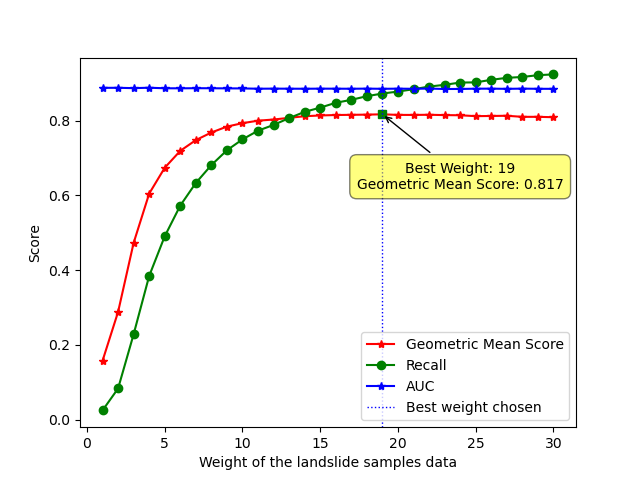
\includegraphics[width=12cm]{Definitions/Fig_Weight_LGBM.png}
  \caption{Misclassification weights of the WLightGBM models.}
  \label{Fig_Weight}
\end{figure}

\begin{figure}
  \centering
  \subfigure[LR model]{
  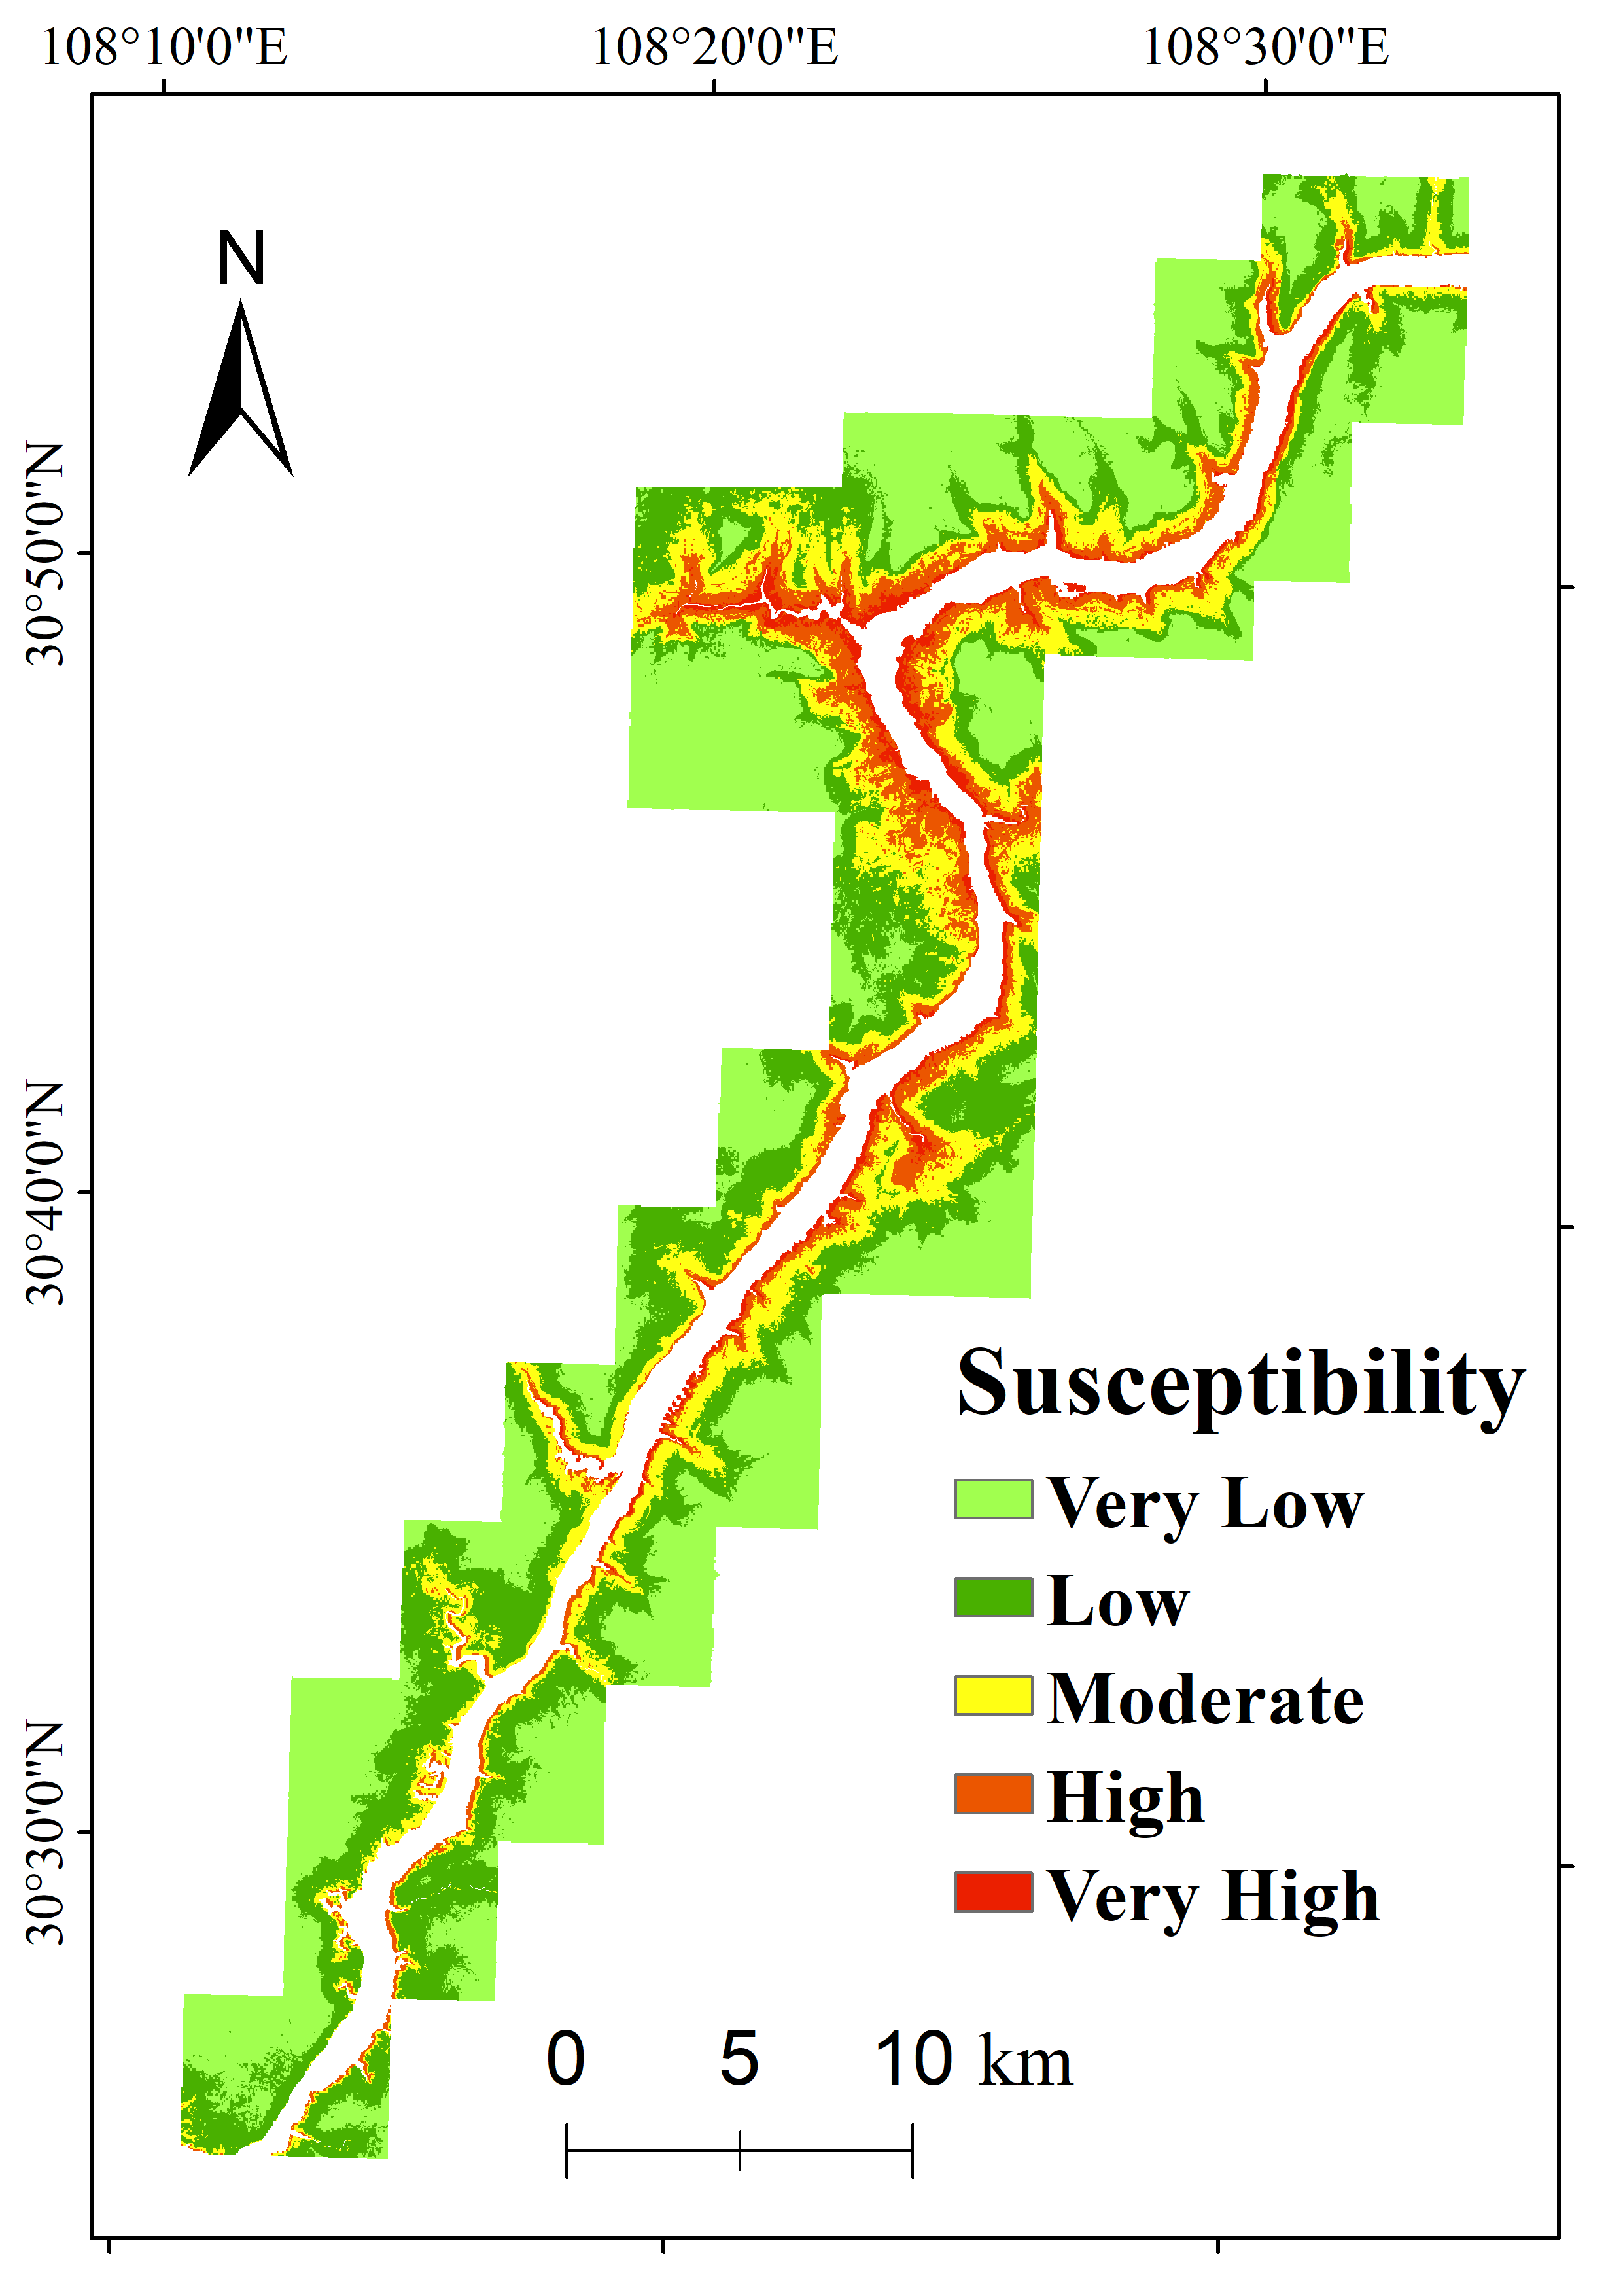
\includegraphics[width=4.6cm]{Definitions/LSM_LR.png}
  }
  \quad
  \subfigure[WLR model]{
  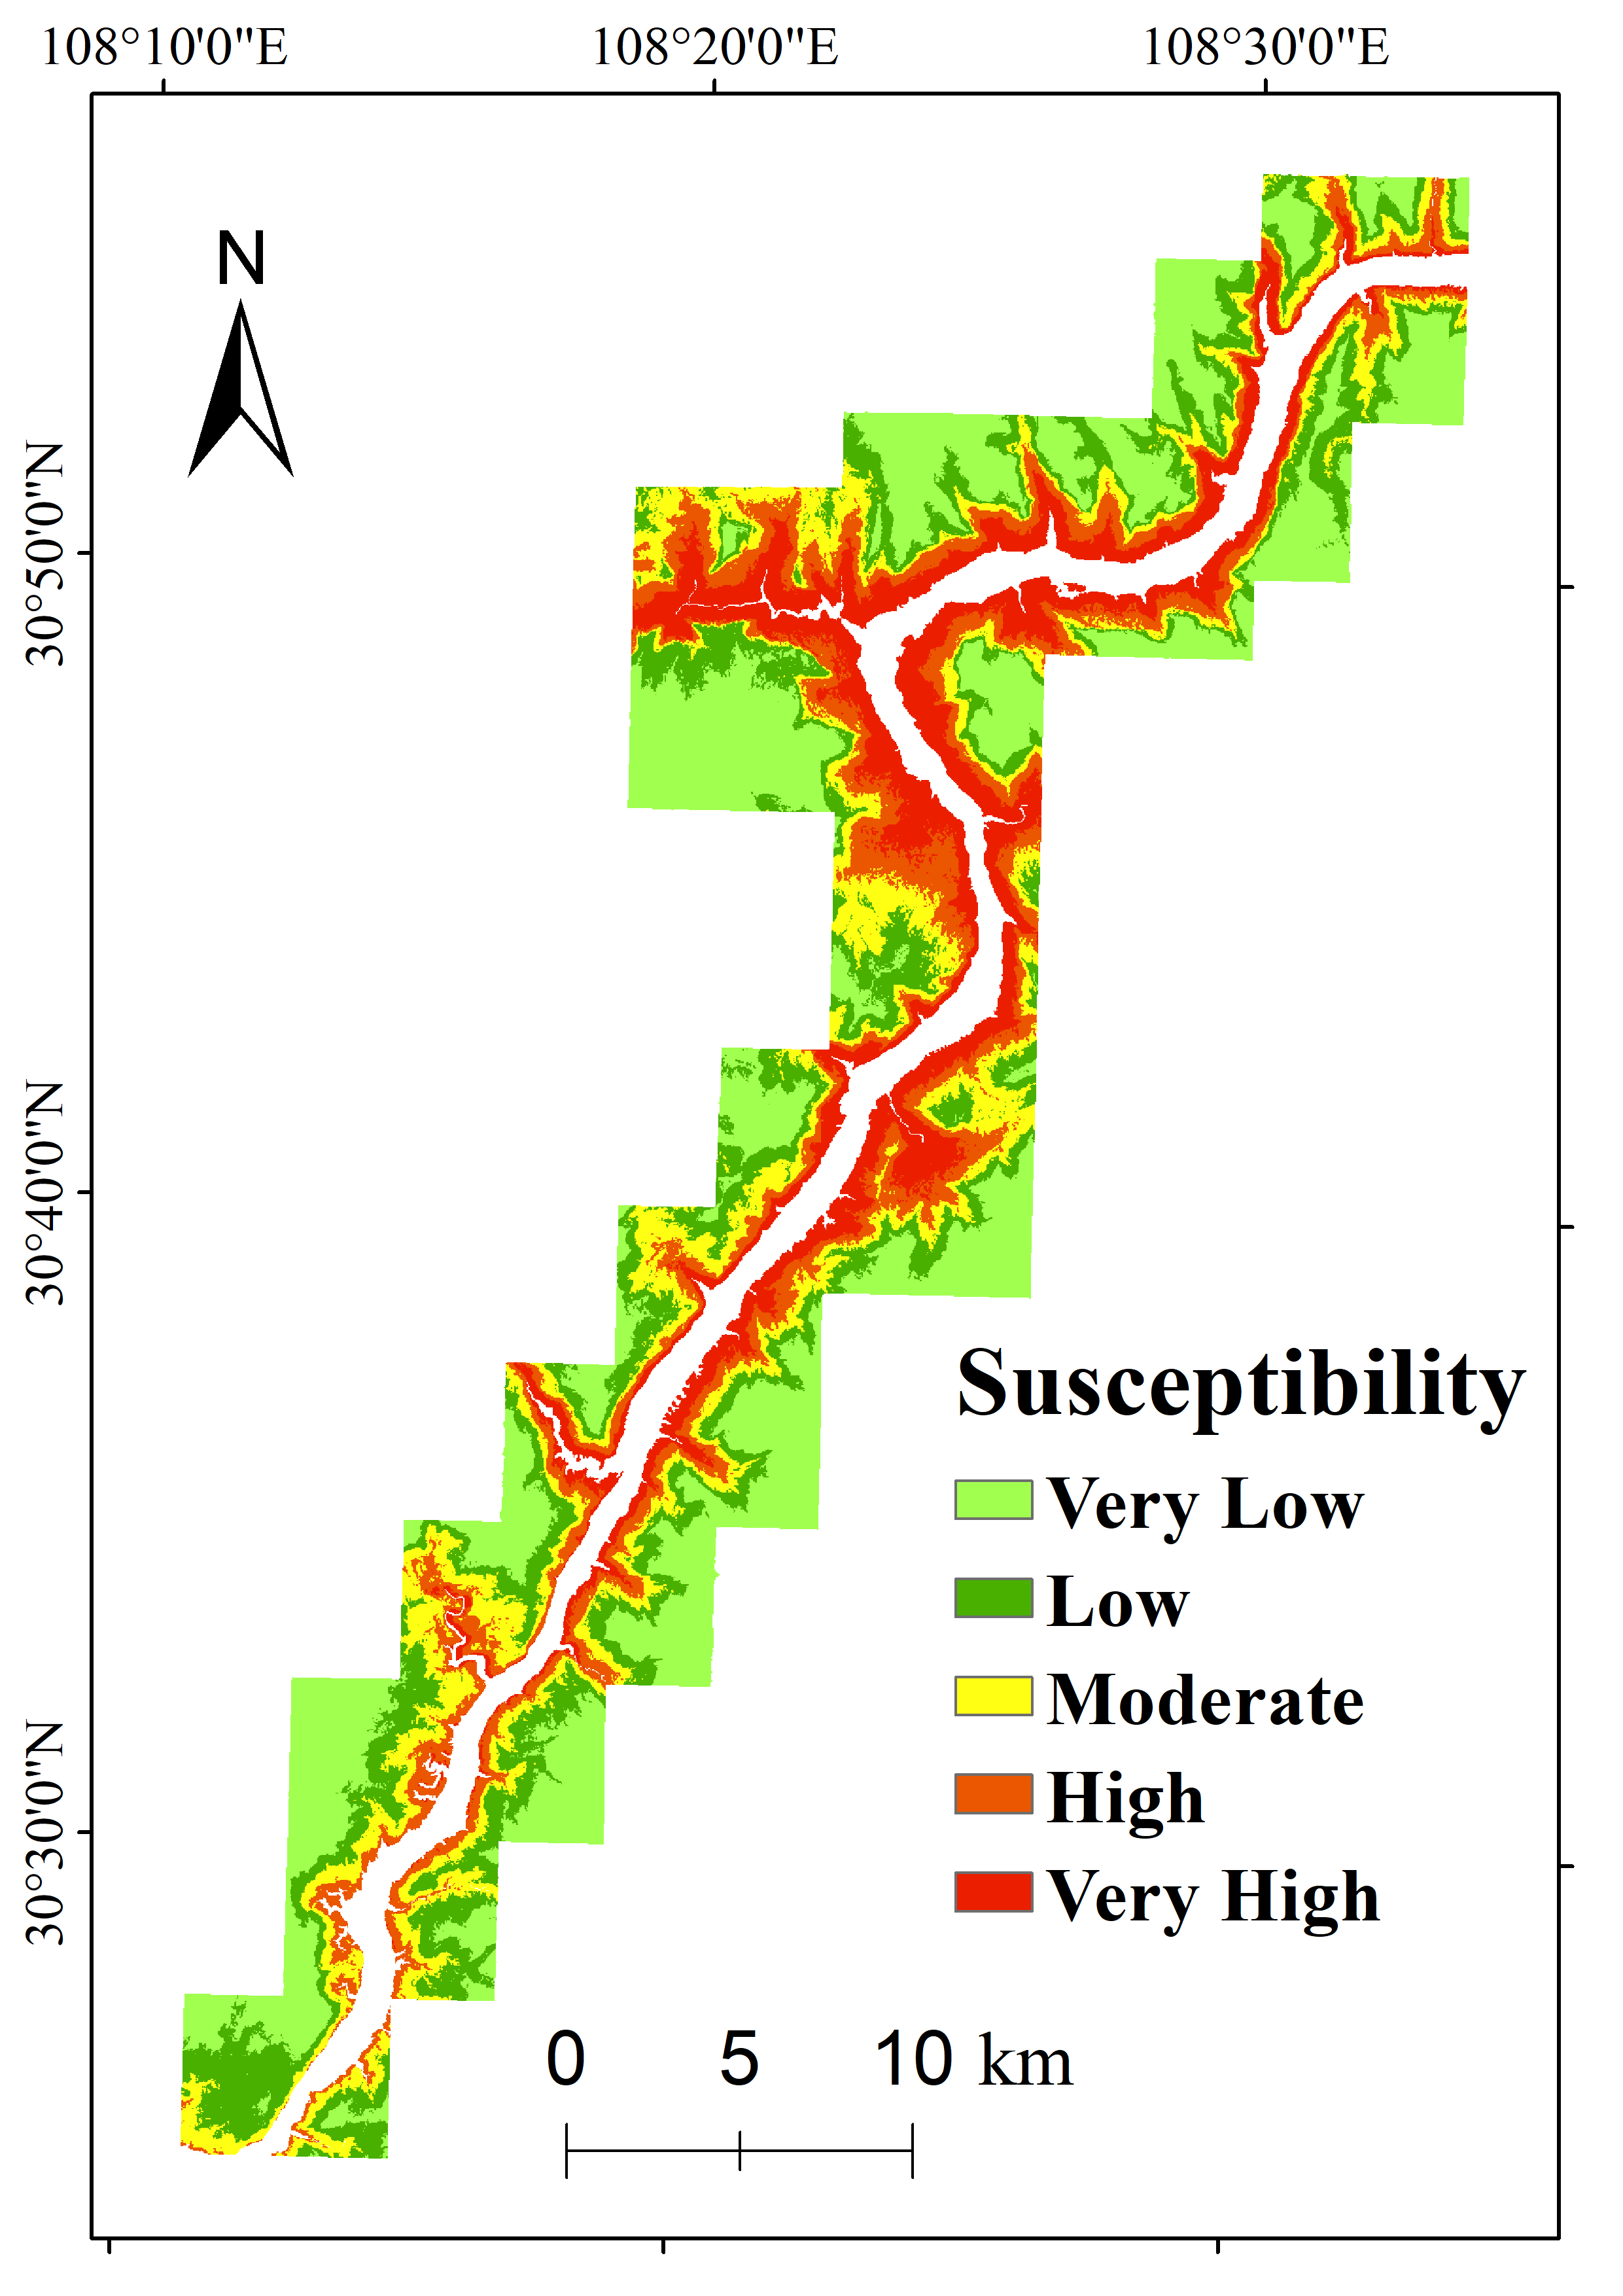
\includegraphics[width=4.6cm]{Definitions/LSM_WLR.png}
  }
  \quad
  \subfigure[LightGBM model]{
  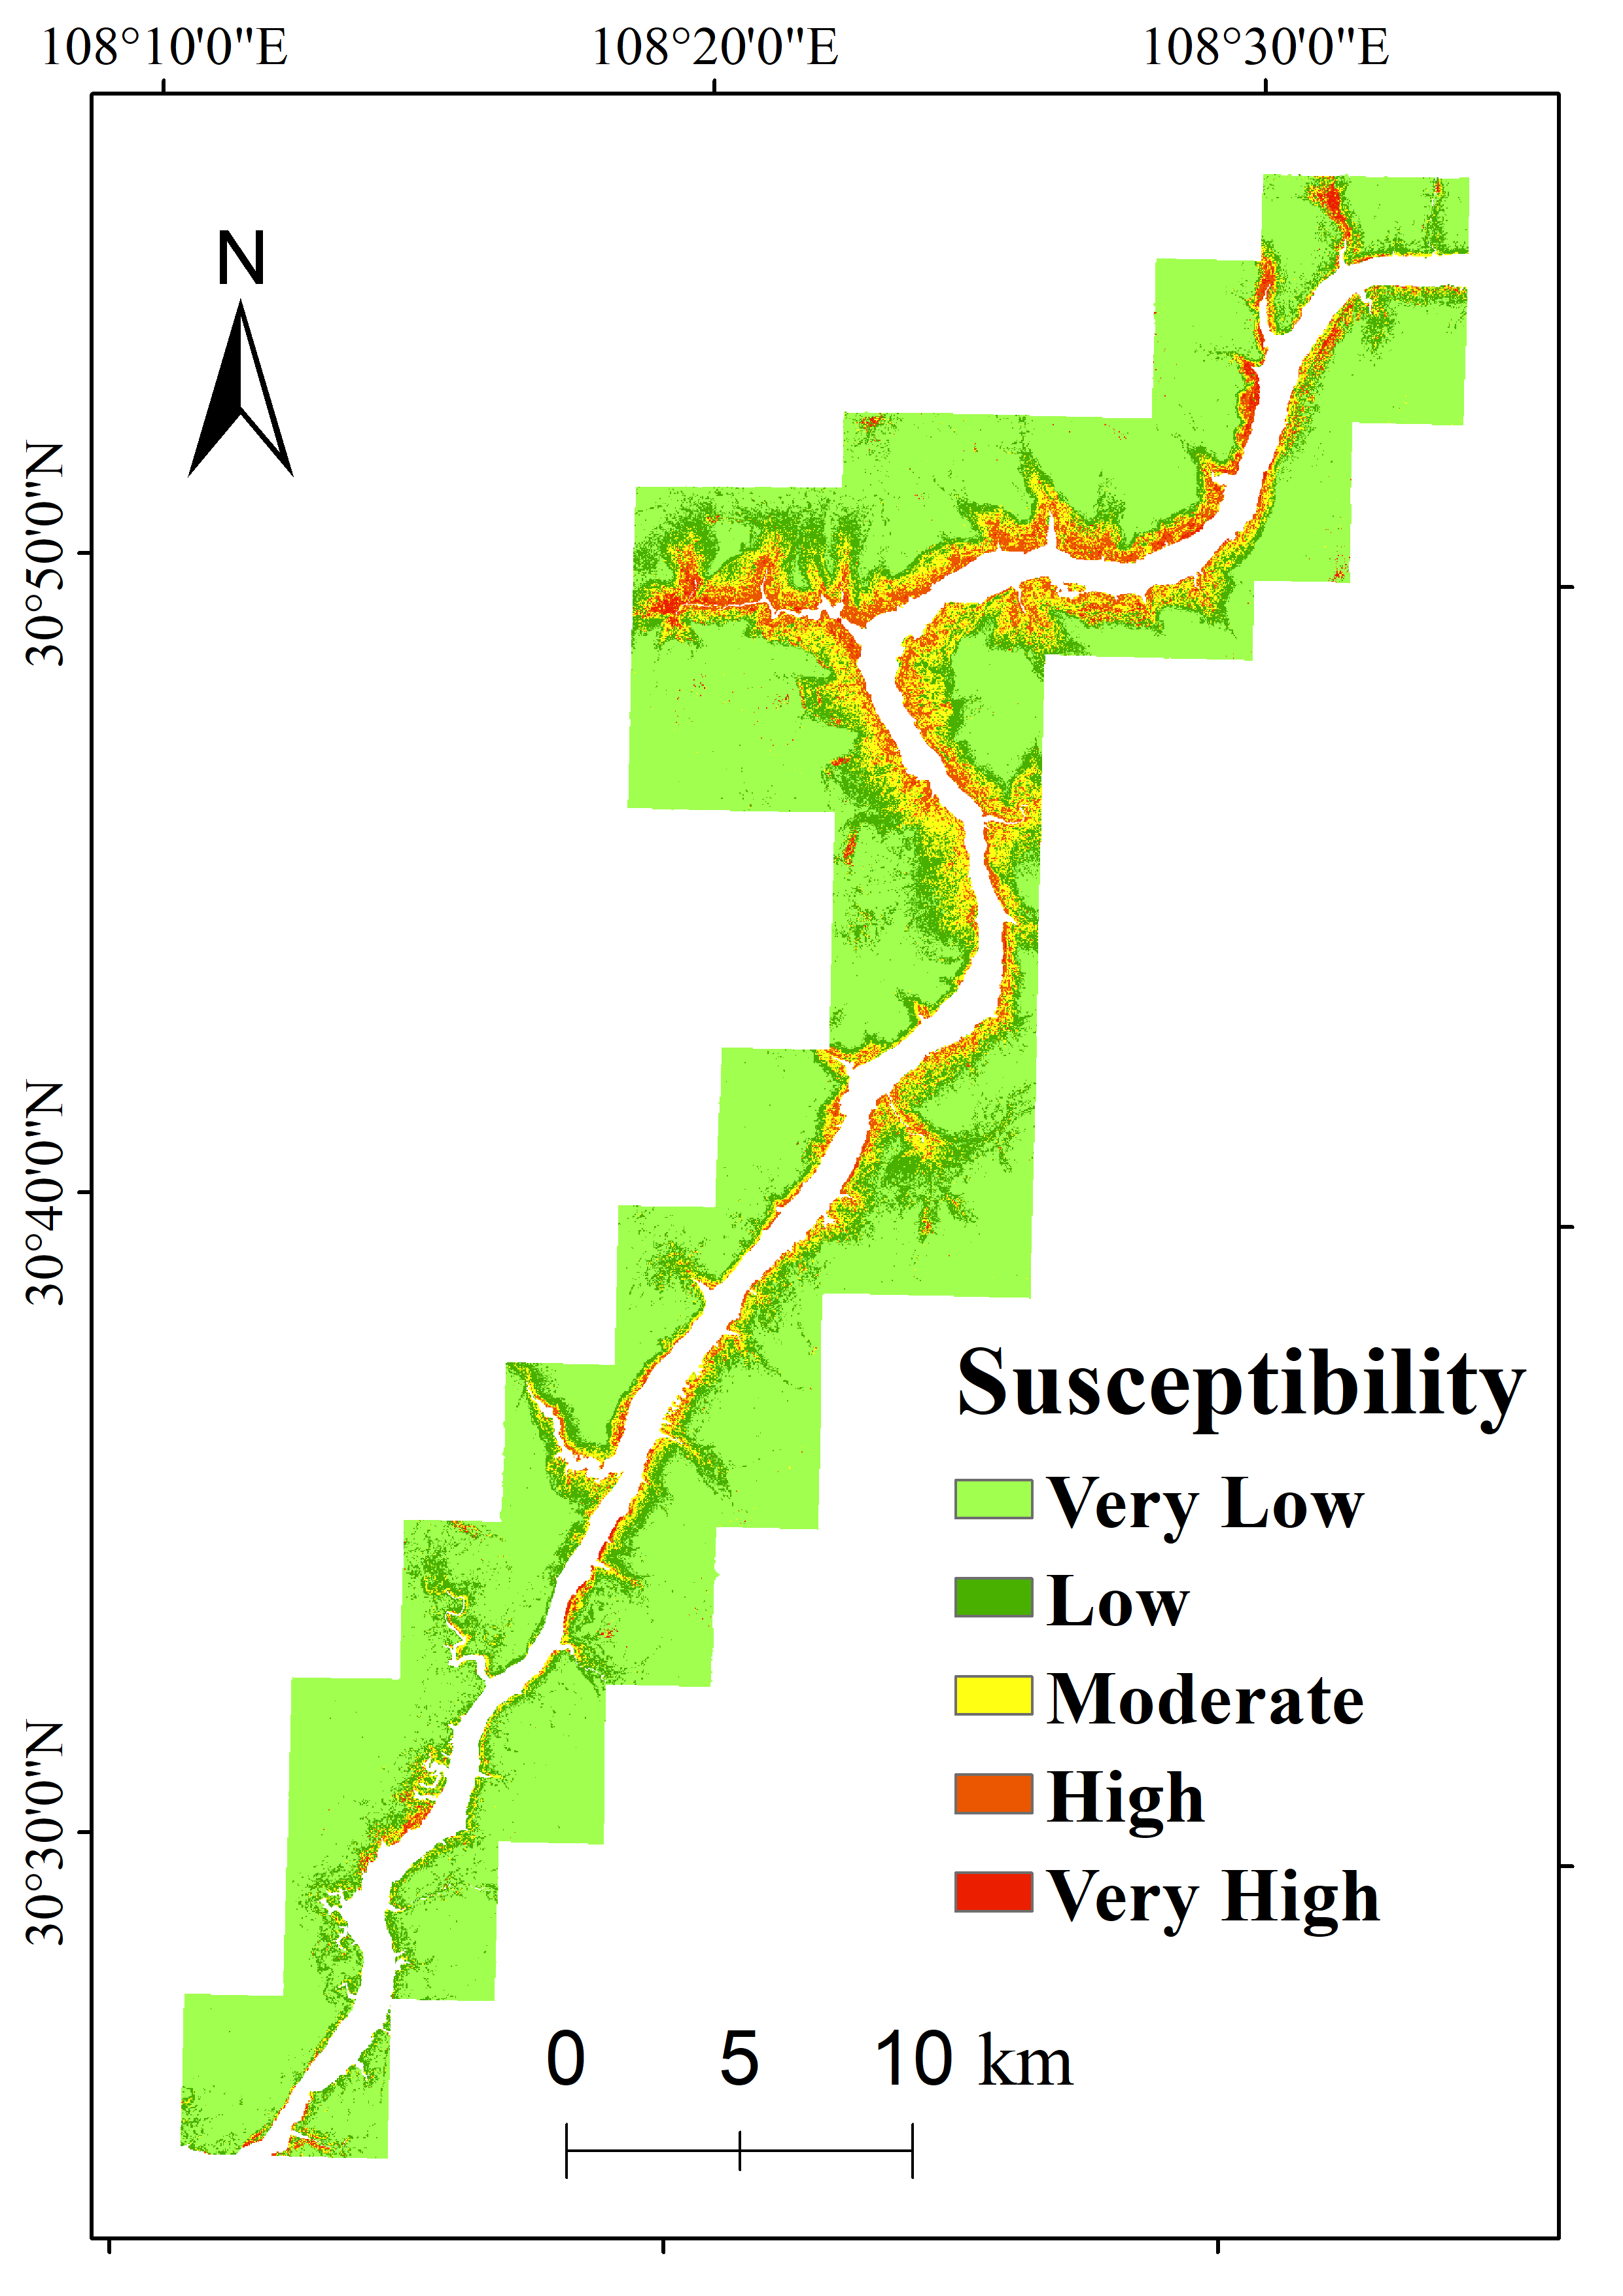
\includegraphics[width=4.6cm]{Definitions/LSM_GBDT.png}
  }
  \quad
  \subfigure[WLightGBM model]{
  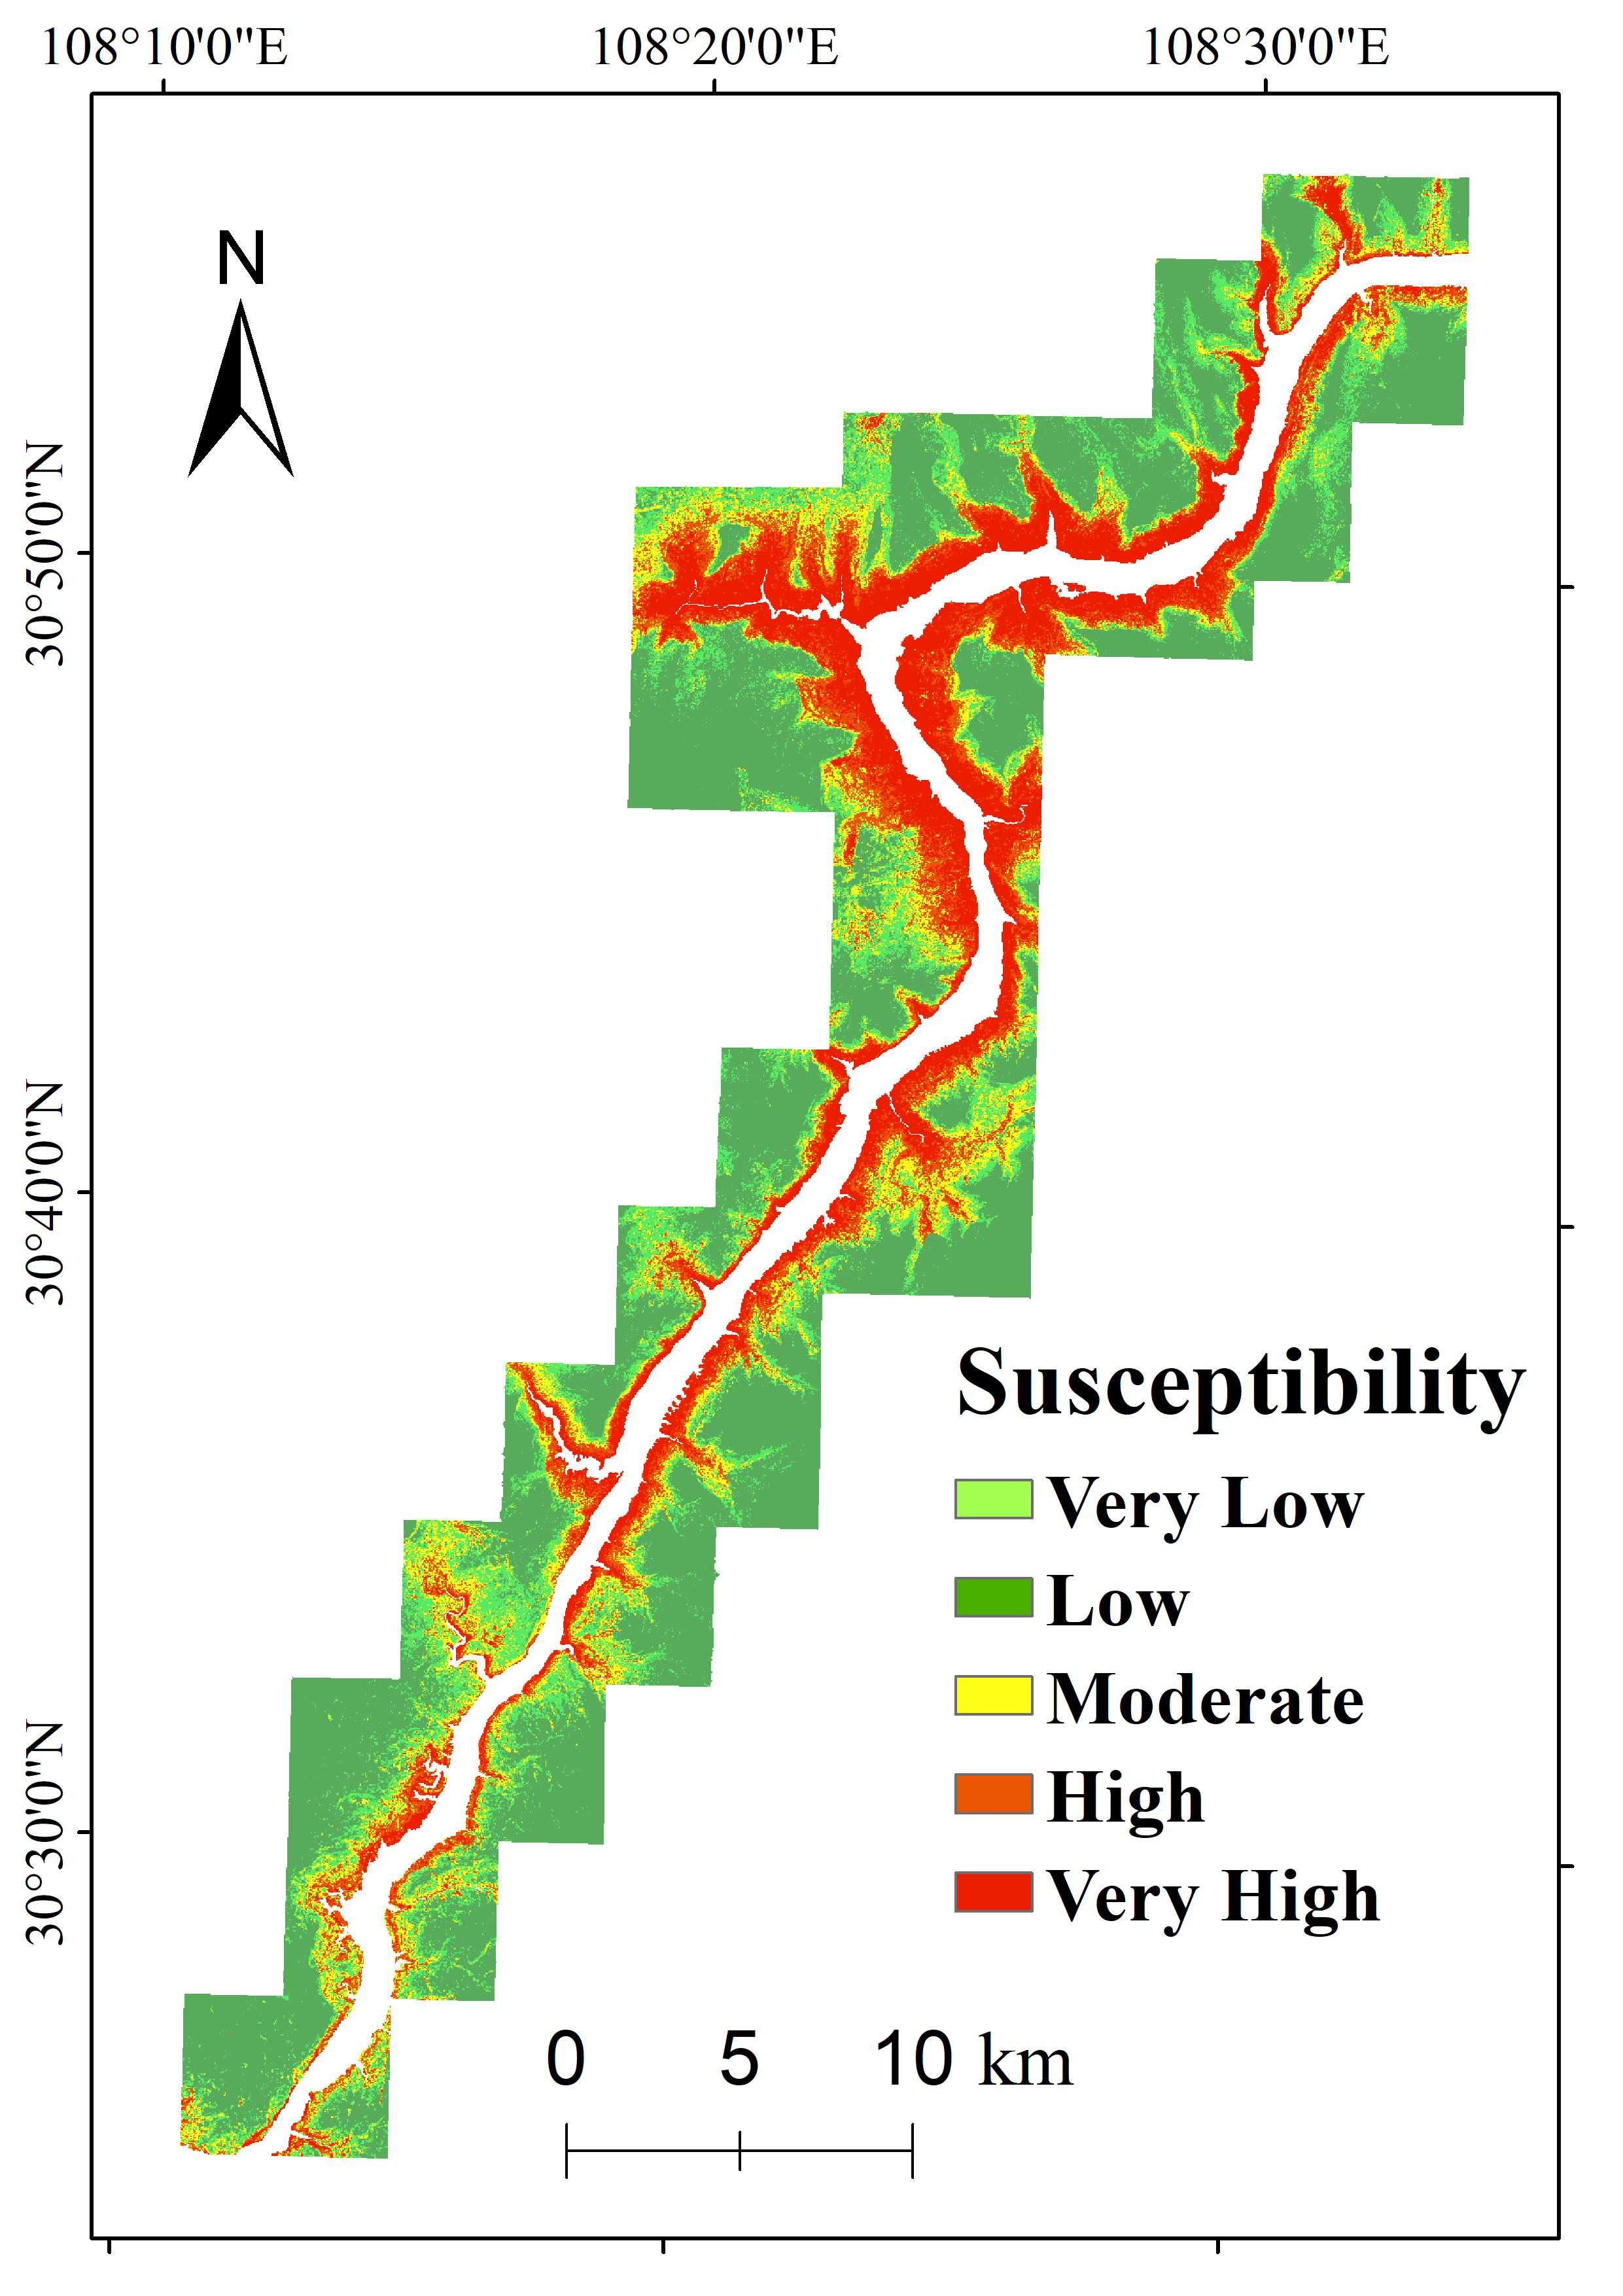
\includegraphics[width=4.6cm]{Definitions/LSM_WGBDT.png}
  }
  \quad
  \subfigure[RF model]{
  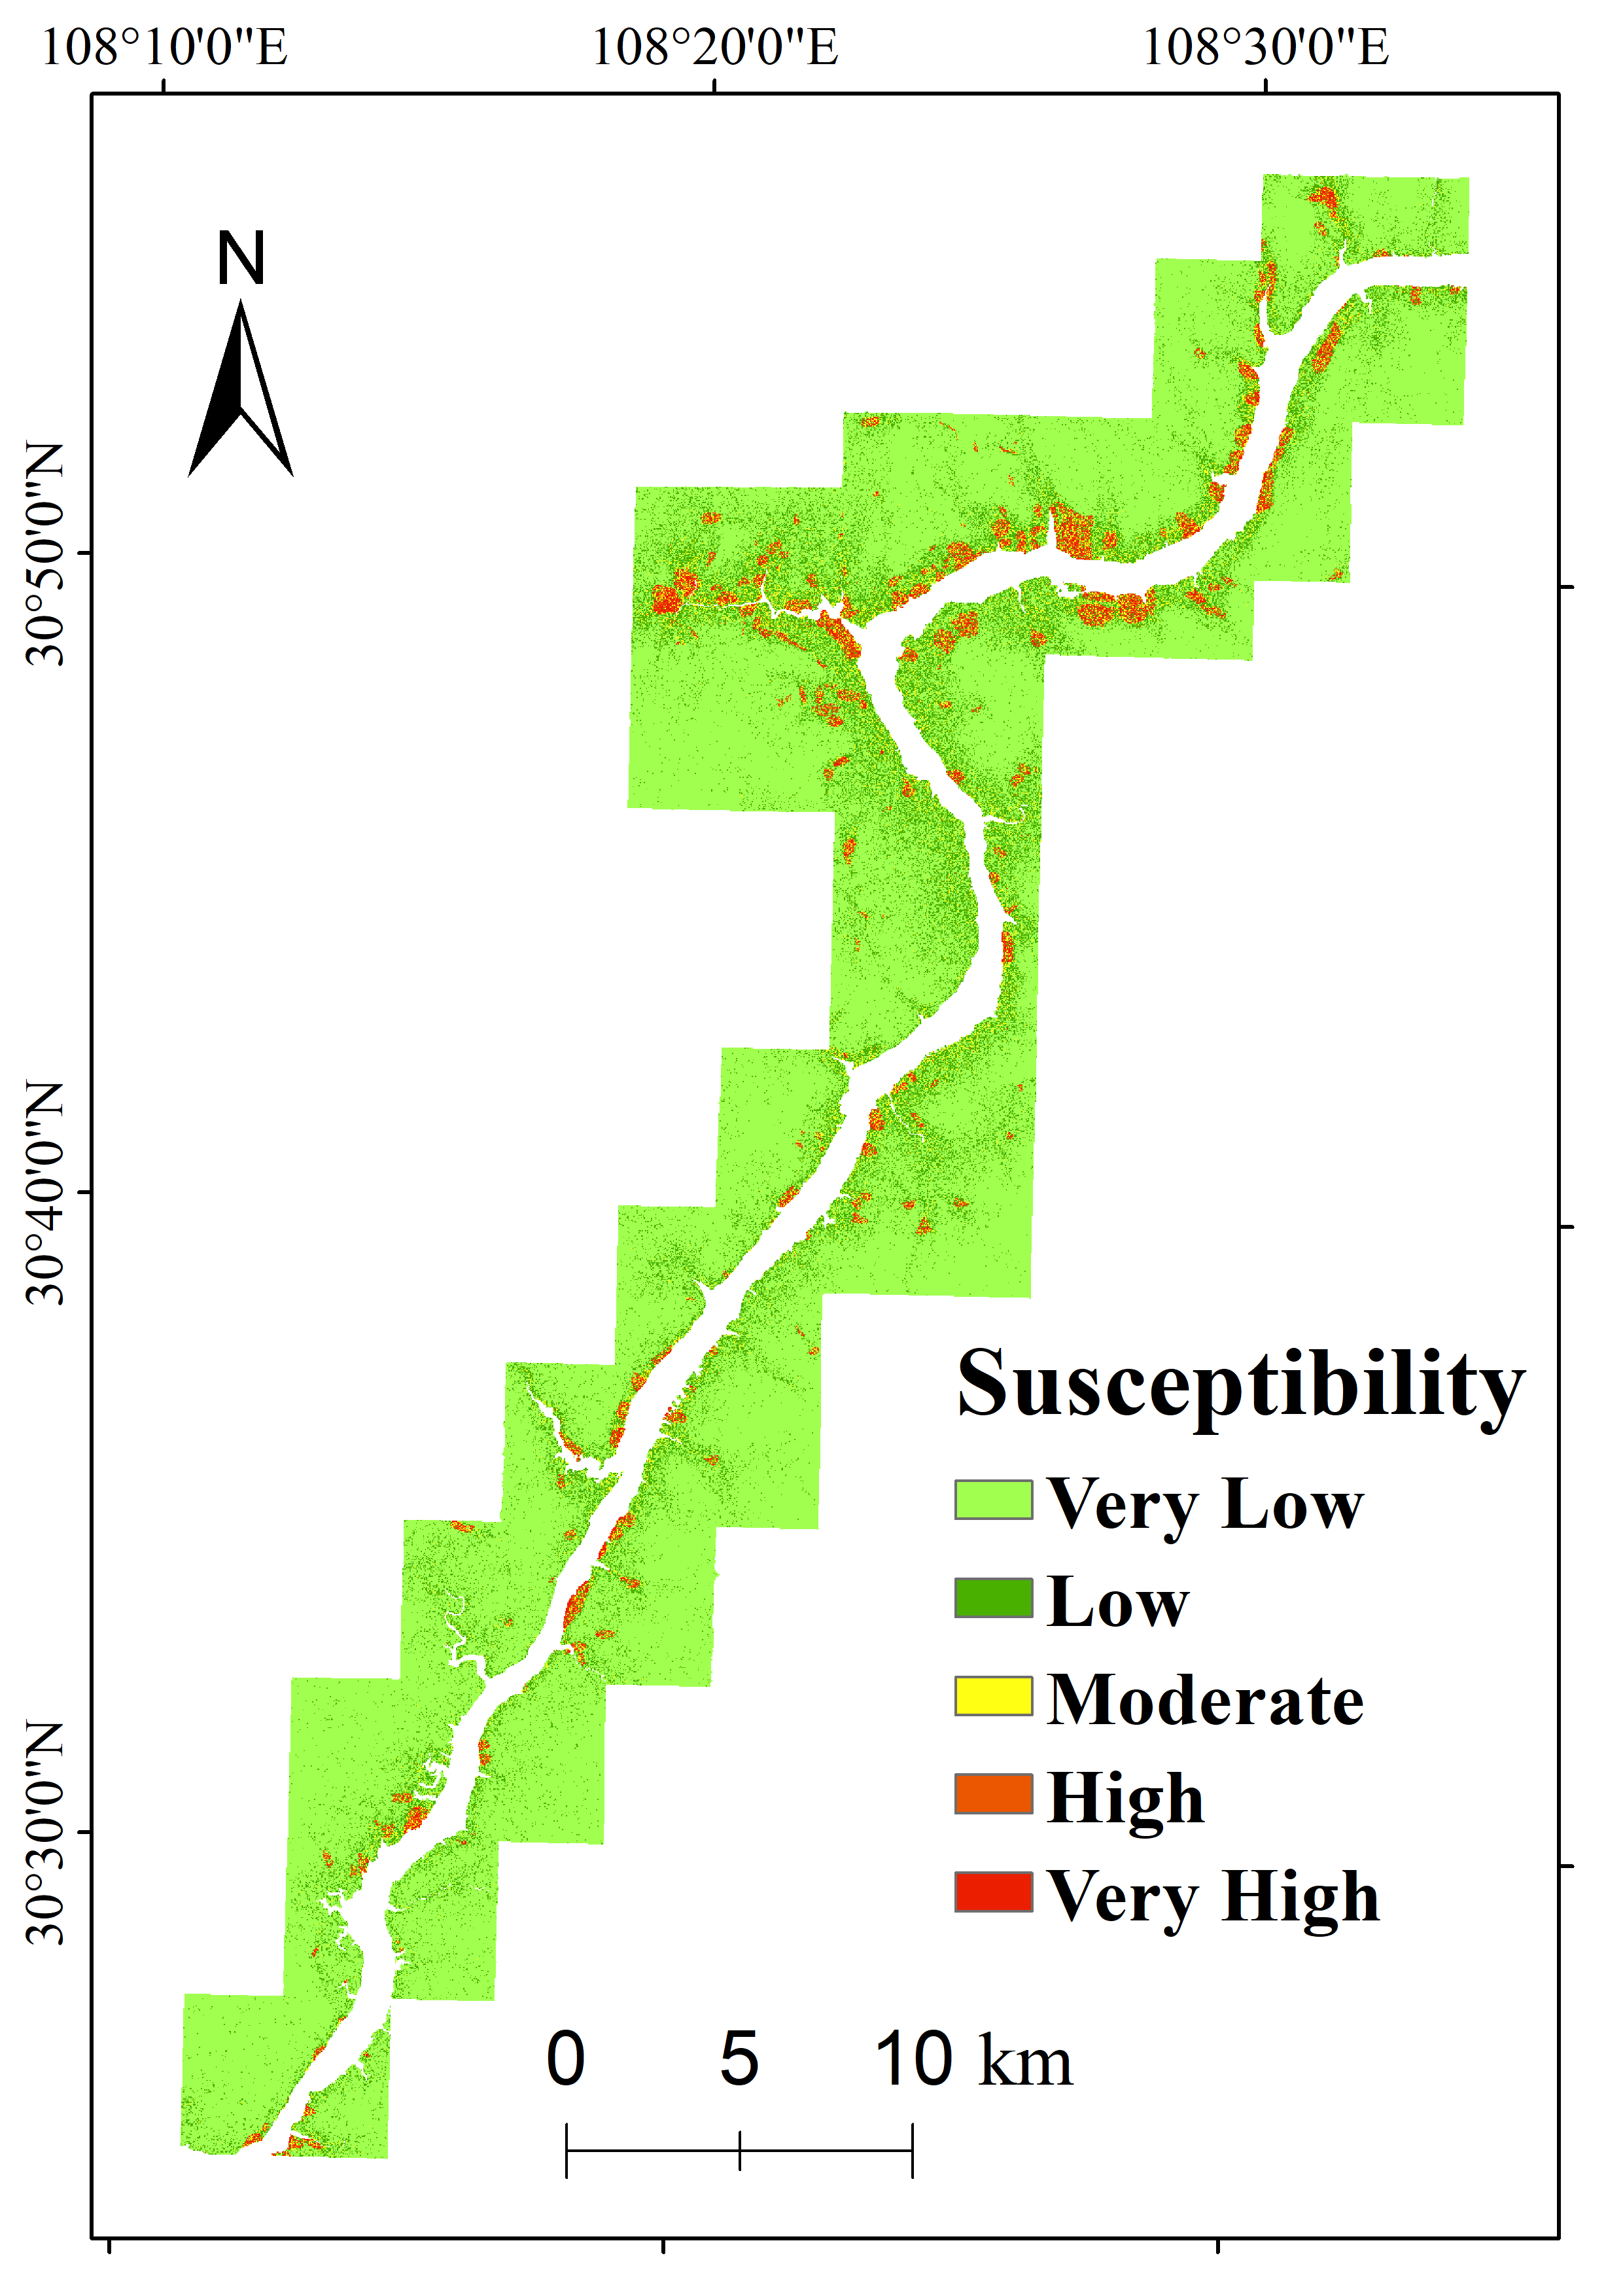
\includegraphics[width=4.6cm]{Definitions/LSM_RF.png}
  }
  \quad
  \subfigure[WRF model]{
  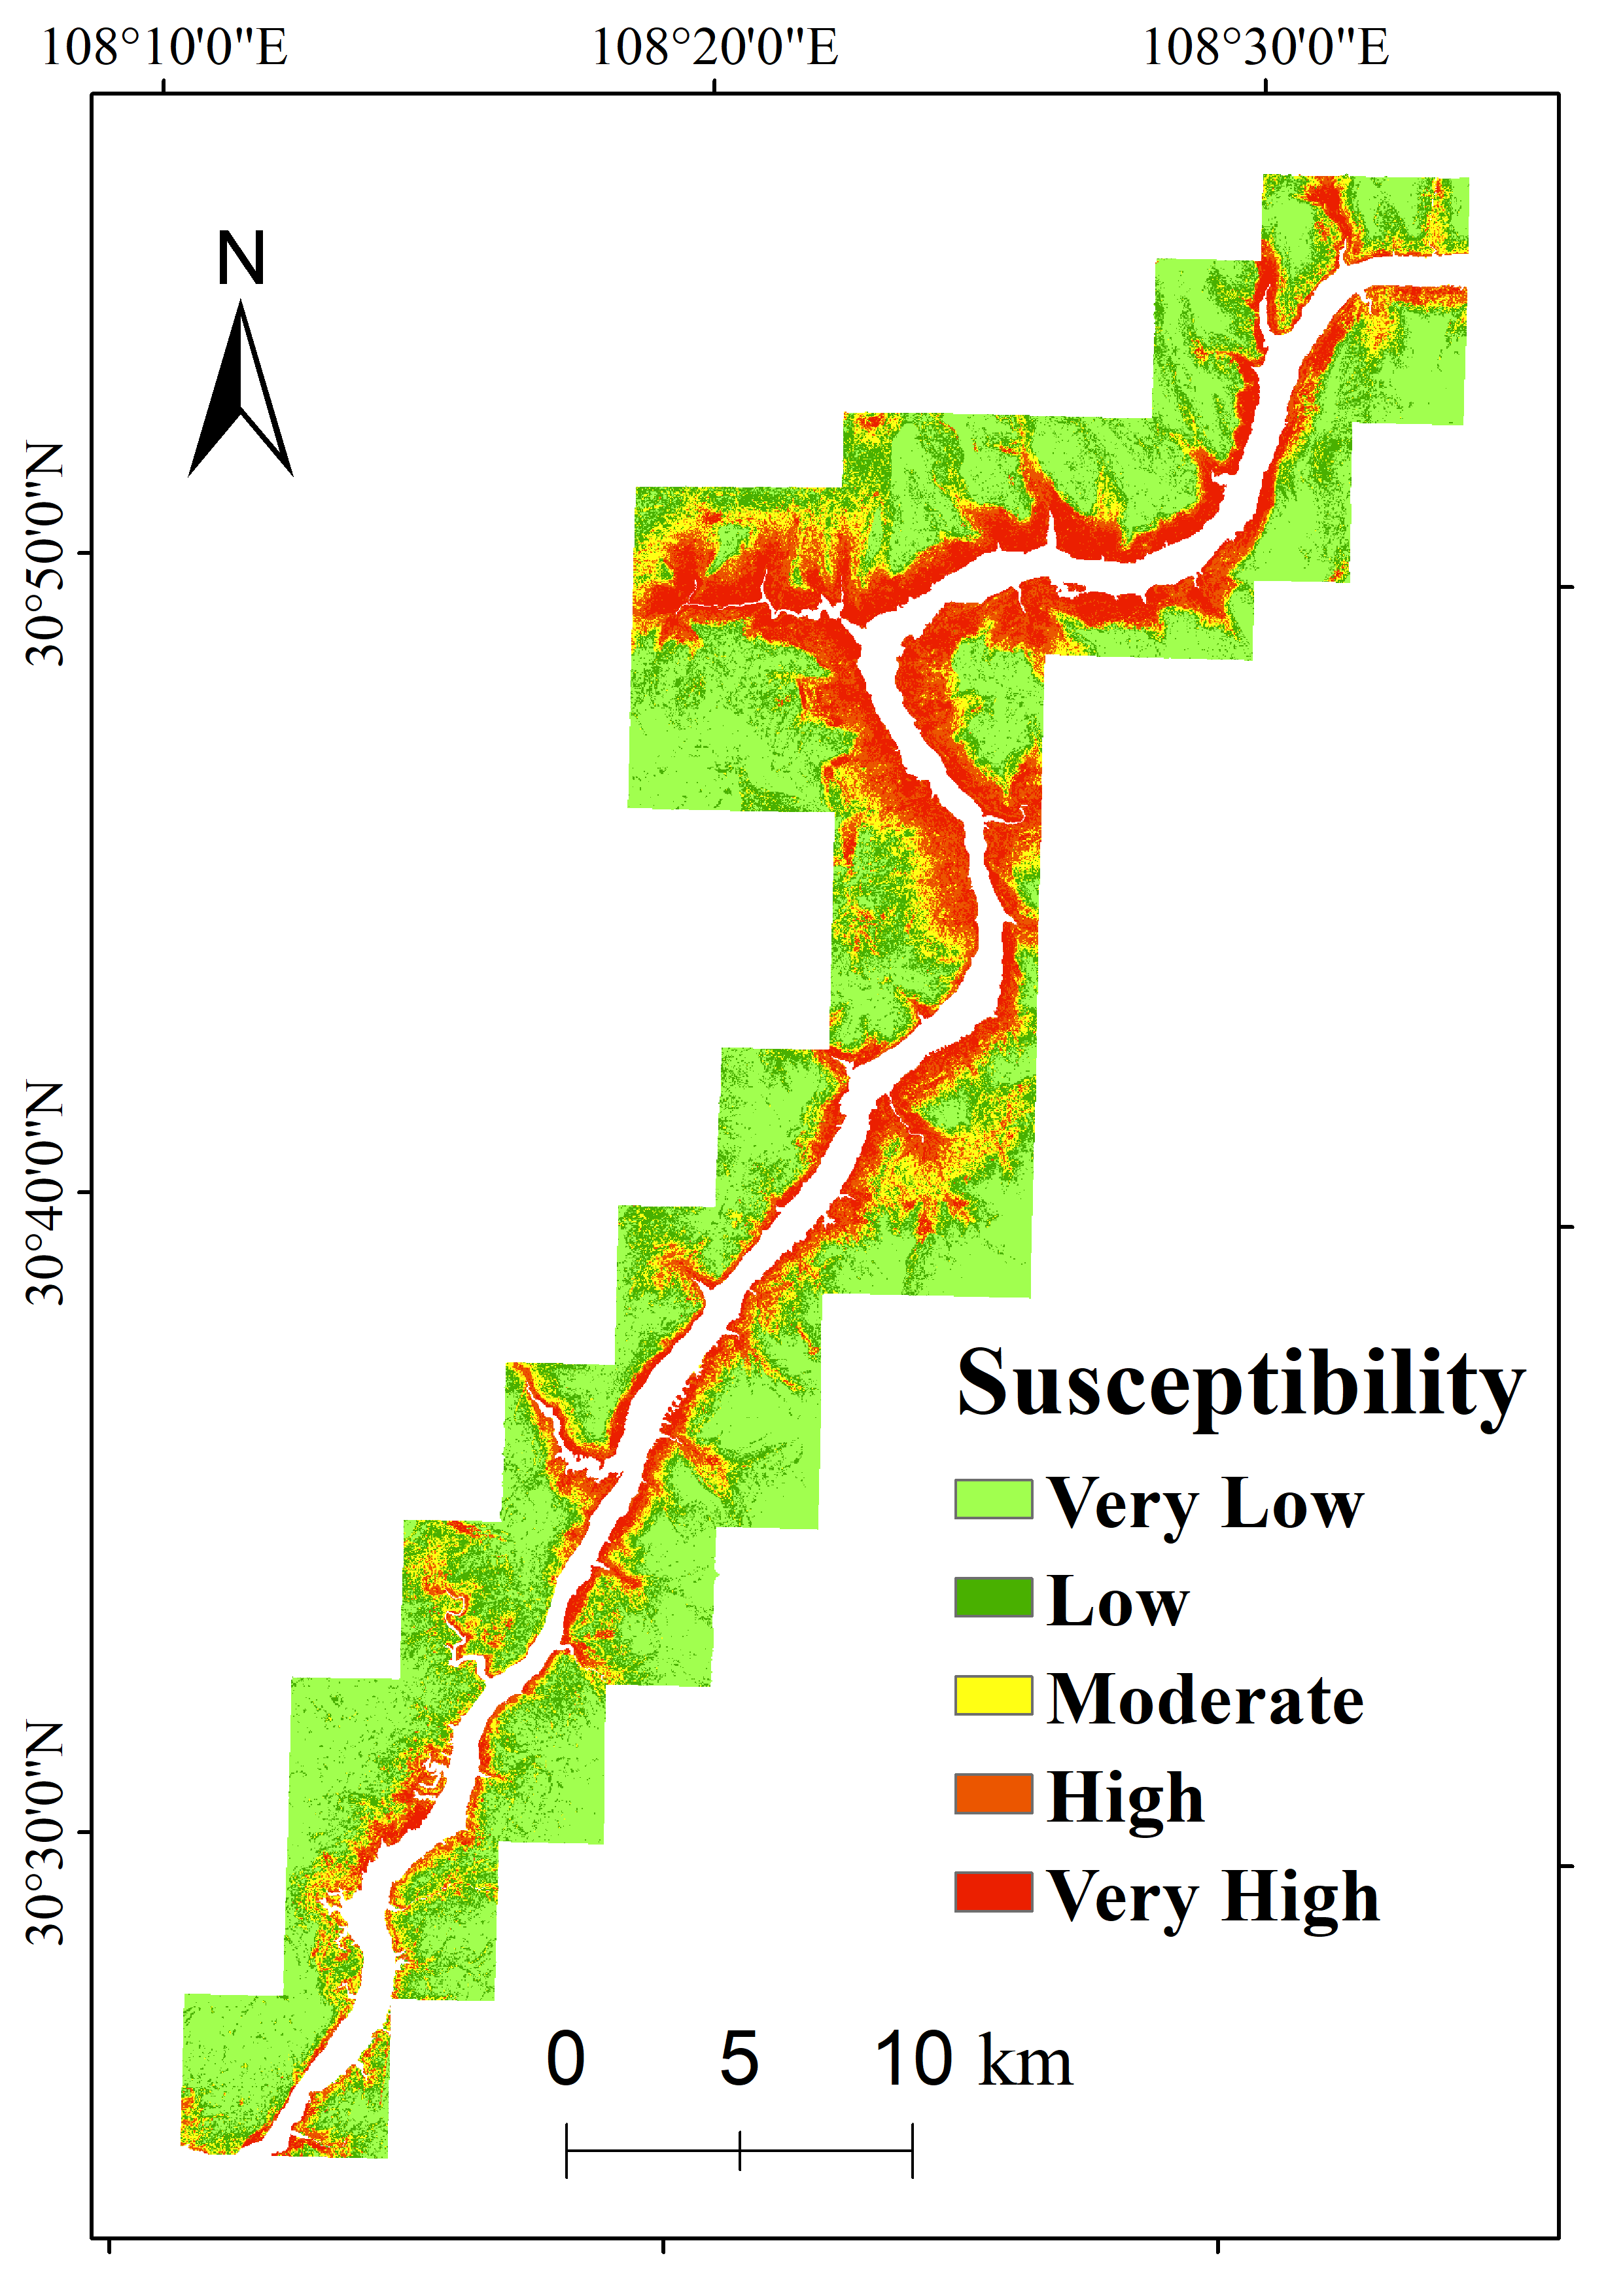
\includegraphics[width=4.6cm]{Definitions/LSM_WRF.png}
  }
  \caption{LSM results of 6 models. (a) LSM using LR model. (b) LSM using WLR model. (c) LSM using LightGBM model. (d) LSM using WLightGBM model. (e) LSM using RF model. (f) LSM using WRF model.}
  \label{LSM_Results}
\end{figure}
% \unskip

\begin{figure}
\centering
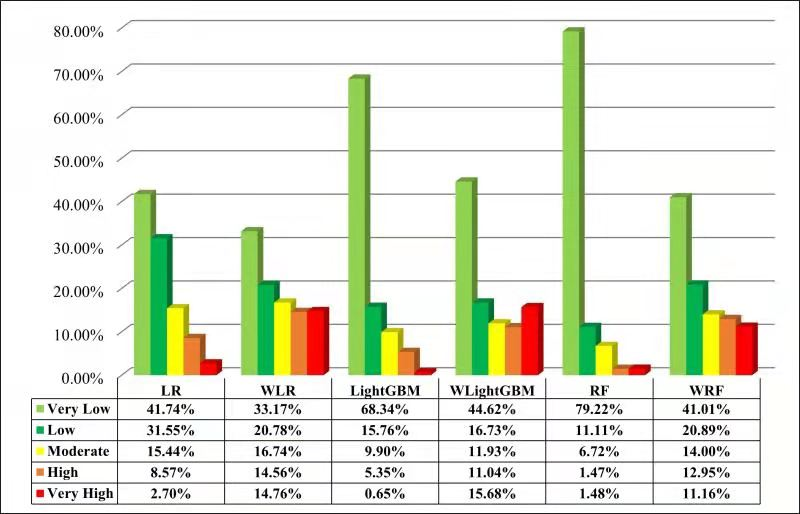
\includegraphics[width=12 cm]{Definitions/Fig_LPI.jpg}
\caption{Distribution ratio of different landslide susceptibility classes for 6 models.}
\label{Fig_distribution}
\end{figure} 

\begin{figure}
  \centering
  \includegraphics[width=12 cm]{Definitions/Fig_ROC_All.png}
  \caption{The ROC curve of 6 LSM models.}
  \label{Fig_ROC_All}
\end{figure} 
>>>>>>> d17d830d74a41a28a19dec78c81ba8068dd4bd0f

\newpage

\textbf{Code availability section}

ArcGIS 10.8 and QGIS 3.16 were used to extract landslide factors, visualize landslide factors and export result maps.

The source codes are available for downloading at the link:
https://github.com/songyingxu/LspModelsForCageo


\bibliographystyle{cas-model2-names}
\bibliography{bibliography} 

\end{document}

